% Capítulo II
\chapter{Operações Fundamentais da Aritmética}

\newpage
\section{Adição}

Ou \textbf{soma}, para os íntimos. Primeiramente, vamos começar com a operação mais fundamental da matemática, a partir da qual podemos encontrar todas as outras. 

\subsection{Lei do elemento zero/nulo}

Por mais óbvio que possa parecer, vamos definir que: a soma de qualquer número “N” com “zero” será igual a “N”. Em outras palavras, quando somamos um número qualquer com zero, o resultado será sempre o próprio número:

\begin{equation}
    N + 0 = N
\end{equation}

\begin{tcolorbox}[title=IMPORTANTE]
    Toda vez que aparecer um número entre parenteses na frente de uma equação, ele serve para te informar qual é o número dela. Exemplo: (2.1) significa que é a primeira equação do capítulo 2; (2.45) significa que é a equação 45 (existem 44 antes dela) do capítulo 2.
\end{tcolorbox}


\subsection{Propriedade comutativa}

Essa propriedade nos diz que a ordem em que somamos dois números não altera o valor final dessa soma. Ou seja, sejam A e B dois números quaisquer:

\begin{equation}
    A+B=B+A
\end{equation}

Perceba que não faz diferença nenhuma se escrevermos primeiro o termo A ou o termo B.\\
\begin{exemplo}
%\begin{tcolorbox}[title=\textbf{Exemplo}]
Considere A = 2 e B = 3.
    \begin{equation}
        2+3=5 \quad ou \quad 3+2=5
    \end{equation}
Nos dá o mesmo resultado, graças a propriedade comutativa.
%\end{tcolorbox}
\end{exemplo}

\subsection{Propriedade associativa}

A propriedade associativa da adição nos leva a perceber que não importa a ordem que somamos uma \textbf{série de números} (mais de 2 números):\\

Sejam A, B e C três números quaisquer, então:

\begin{equation}
    (A+B)+C=A+(B+C)
\end{equation}

A ideia aqui é mostrar que não existe diferença em somar primeiro A com B e, somente depois, adicionar o valor de C; ou somar primeiro B com C e depois adicionar o valor de A. O nosso resultado será o mesmo.

\begin{exemplo}
%\begin{tcolorbox}[title=\textbf{Exemplo}]
Sejam A = 2, B = 5 e C = 4, então:

    \begin{equation}
        (2+5)+4 \Rightarrow 7 + 4 \Rightarrow 11
    \end{equation}
ou

    \begin{equation}
        2+(5+4) \Rightarrow 2 + 9 \Rightarrow 11
    \end{equation}

Em ambos os casos temos o resultado final igual.
%\end{tcolorbox}
\end{exemplo}

Vejamos agora o dispositivo prático para efetuar uma soma.

\subsection{Dispositivo Prático}

Entenda ``dispositivo prático'' como um procedimento com uma série de regras, que visa tornar operações abstratas mais ``amigáveis''.

Para evitar abordar conceitos que fogem do objetivo dessa apostila “básica”, não faremos uma definição teórica para esse dispositivo prático, somente exemplos numéricos. 
% Veremos isso com mais calma em outra oportunidade. Apesar do nome sugerir algo complexo e difícil, é algo que costumamos aprender nos anos iniciais da escola, e que muitas vezes já é até ``intuitivo''.

Até o momento, nós apenas estudamos algumas das somas mais “simples” que muitas vezes podemos até fazer contando os dedos das mãos - e dos pés também, se preferir. Vejamos agora alguns exemplos de somas menos triviais.\\

\begin{exemplo}[Dispositivo Prático da Adição]
\label{exemplo_disp_adicao}
Para explicar o método, comecemos com uma soma mais\(\dots\) didática. Se quisermos somar 13 e 11, por exemplo, montaremos sempre nosso dispositivo de soma da seguinte maneira: 

\begin{figure}[H]
    \centering
    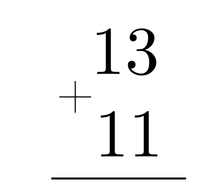
\includegraphics[scale=0.5]{imagens/soma_11_13_1.png}
    \label{fig:soma_11_13_1}
\end{figure}

Aplicando o mesmo procedimento, colocamos o número maior (13) por cima e o menor (11) por baixo, com seus “últimos números” se encontrando. Porém, \textbf{como vimos no capítulo anterior}, podemos utilizar um \textit{matematiquês} mais elaborado para representar esse procedimento:

Colocamos os \textbf{algarismos} das \textbf{unidades} abaixo dos algarismos unidades, dezenas abaixo de dezenas, centenas abaixo de centenas, e assim em diante. 

Porém, nesse exemplo (\(13 + 11\)) só temos até as dezenas. Veja: 

    \begin{itemize}
        \item 13 = 10 + 3 = 1 dezena e 3 unidades
        \item 11 = 10 + 1 = 1 dezena e 1 unidade
    \end{itemize}

A partir disso, faremos as somas individuais dois a dois (o número/algarismo de cima com o de baixo), sempre começando da direita para esquerda.

Começando da direita, a primeira soma que temos é 3 + 1, que nos dá o resultado 4, o qual escrevemos abaixo da linha preta e partimos para a próxima adição.

\begin{figure}[H]
    \centering
    
\includegraphics[scale=0.5]{imagens/soma_11_13_2.png}
    \label{fig:soma_11_13_2}
\end{figure}

Agora, temos a soma 1 + 1, que nos dá o resultado 2. Novamente, o escrevemos abaixo da linha preta, como mostrado a seguir:

\begin{figure}[H]
    \centering
    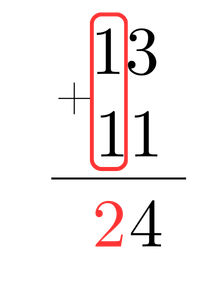
\includegraphics[scale=0.5]{imagens/soma_11_13_3.png}
    \label{fig:soma_11_13_3}
\end{figure}

Como não temos mais algarismos para somar, definimos nosso resultado como o número que aparece abaixo da linha preta: o resultado da soma de \textbf{11} mais \textbf{13} é igual a \textbf{24}.
\end{exemplo}

Vejamos um exemplo um \textit{pouco} mais interessante.

\begin{exemplo}
    Soma de 16 e 15:

    Aplicando o mesmo procedimento visto em \ref{exemplo_disp_adicao} na página \pageref{exemplo_disp_adicao}, colocamos o número maior por cima e o menor por baixo, com os algarismos das unidades se encontrando. Ou seja, ``6'' e ``5'' (unidades) um abaixo do outro, e ``1'' e ``1'' que são dezenas, um abaixo do outro.

    \begin{figure}[H]
        \centering
        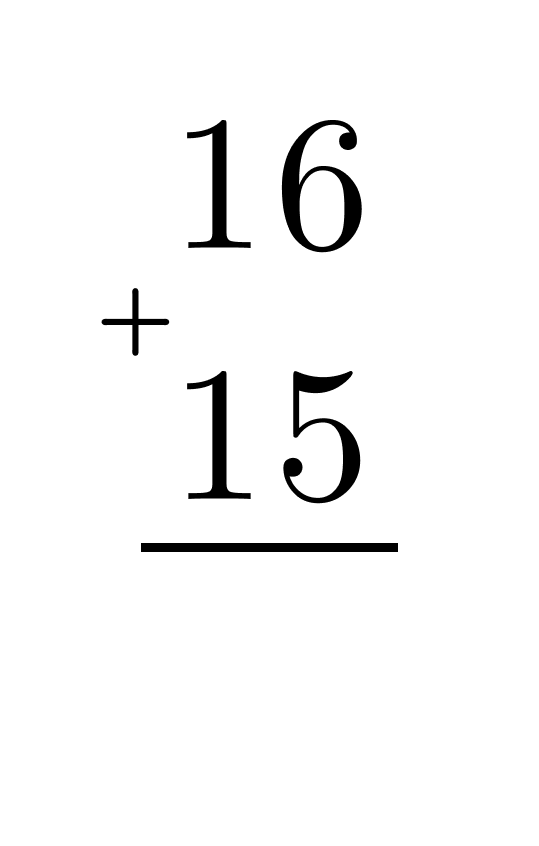
\includegraphics[width=0.25\linewidth]{imagens/soma_16_15_1.png}
        \label{fig:soma_16_15_1}
    \end{figure}

    Começando pela direita, note que a nossa primeira soma (6 + 5) nos dá um resultado \textbf{11}. Porém, abaixo da linha só temos espaço para números com um dígito/algarismo (ou seja, de 0 a 9).

    \begin{figure}[H]
        \centering
        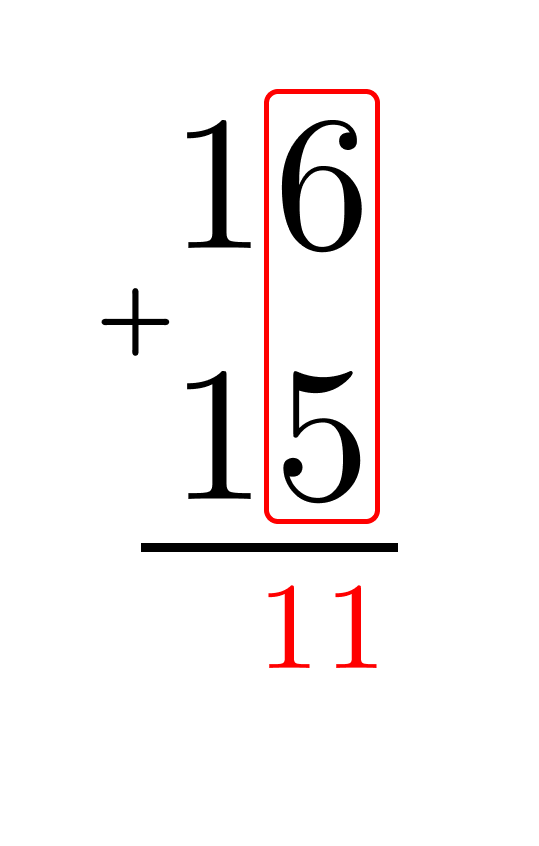
\includegraphics[width=0.25\linewidth]{imagens/soma_16_15_2.png}
        \label{fig:soma_16_15_2}
    \end{figure}

    O procedimento, então, nos diz para fazer o seguinte: separamos o \textbf{11} em dois algarismos \textbf{1}. O da direita permanece embaixo da linha, e o da esquerda é colocado acima do próximo número que faremos a soma.

    \begin{figure}[H]
        \centering
        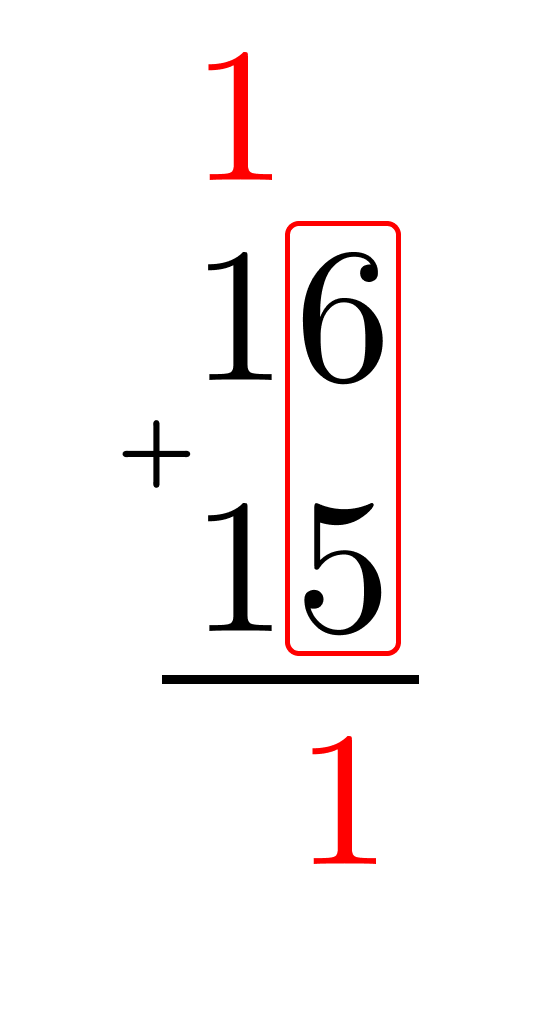
\includegraphics[width=0.25\linewidth]{imagens/soma_16_15_3.png}
        \label{fig:soma_16_15_3}
    \end{figure}

    Da mesma maneira que antes, faremos a soma dos próximos números (incluindo o nosso novo número ``1'' em cima).

    \begin{figure}[H]
        \centering
        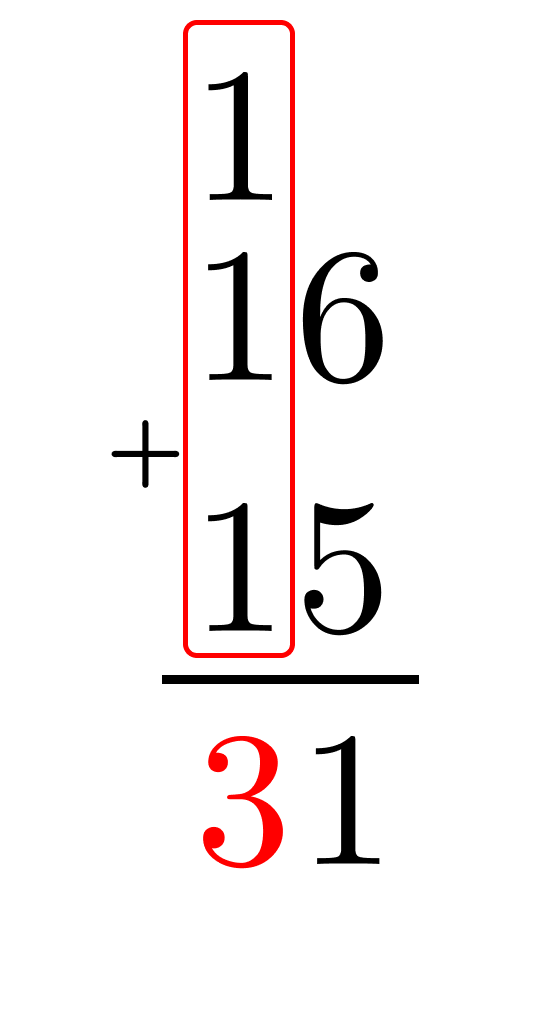
\includegraphics[width=0.25\linewidth]{imagens/soma_16_15_4.png}
        \label{fig:soma_16_15_4}
    \end{figure}

    Como não temos mais números para somar, concluímos que nosso resultado da soma é o número abaixo da linha.
    
    Portanto, o resultado da soma de \textbf{16} mais \textbf{15} é \textbf{31}.
\end{exemplo}

Mais um exemplo.

\begin{exemplo}
    Soma de 125 e 17:

    Aqui não faremos nada de diferente: vamos aplicar o mesmo método utilizado anteriormente, com as mesmas regras.

    \begin{figure}[H]
        \centering
        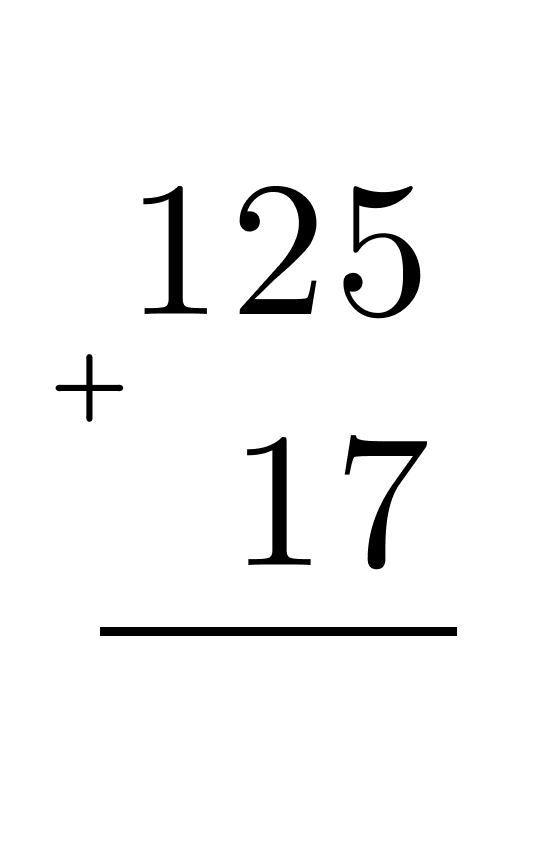
\includegraphics[width=0.25\linewidth]{imagens/soma_125_17_1.png}
        \label{fig:soma_125_17_1}
    \end{figure}

    Também temos o maior número por cima, o menor por baixo, e os algarismos das ``unidades'' se encontrando. Façamos nossa soma.

    \begin{figure}[H]
        \centering
        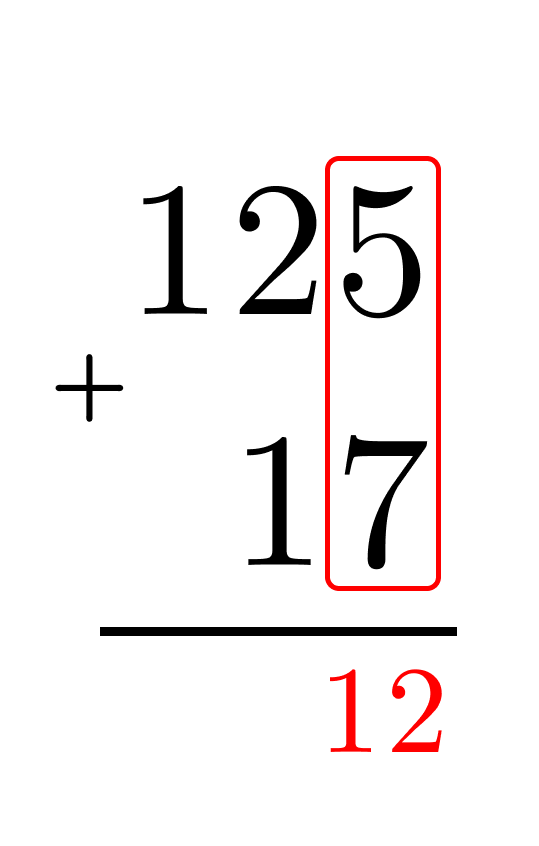
\includegraphics[width=0.25\linewidth]{imagens/soma_125_17_2.png}
        \label{fig:soma_125_17_2}
    \end{figure}

    Novamente, temos o caso da soma 5 + 7 = 12, que resulta em um número de dois dígitos. Vamos separá-lo como havíamos feito para o 11, no exemplo anterior.

    \begin{figure}[H]
        \centering
        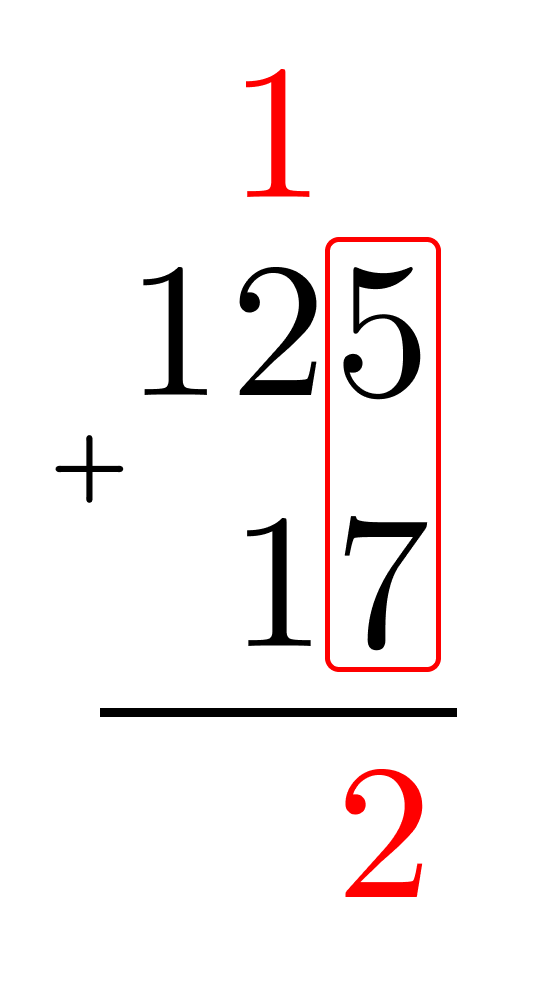
\includegraphics[width=0.25\linewidth]{imagens/soma_125_17_3.png}
        \label{fig:soma_125_17_3}
    \end{figure}

    Passamos para nossa próxima soma da esquerda:

    \begin{figure}[H]
        \centering
        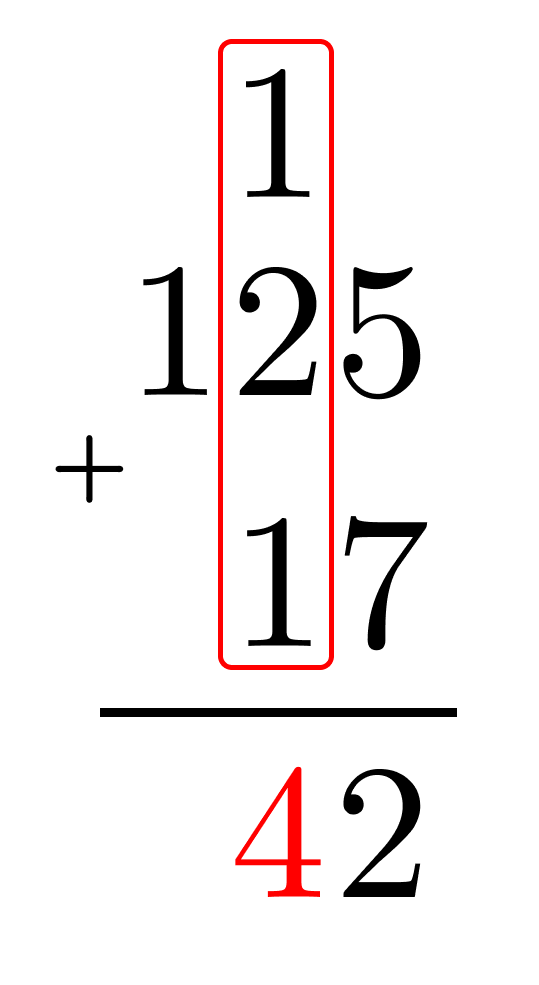
\includegraphics[width=0.25\linewidth]{imagens/soma_125_17_4.png}
        \label{fig:soma_125_17_4}
    \end{figure}

    Agora, temos o número 1 sozinho, mas vamos assumir que há um número 0 abaixo dele (temos que lembrar \textbf{da Lei do Elemento Zero}). Então podemos visualizar o número 17 como 017, o que não mudará em nada nossos cálculos (``zero à esquerda''). Na prática, estamos só adicionando um algarismo das centenas igual a zero no nosso número, para facilitar o raciocínio.

    \begin{figure}[H]
        \centering
        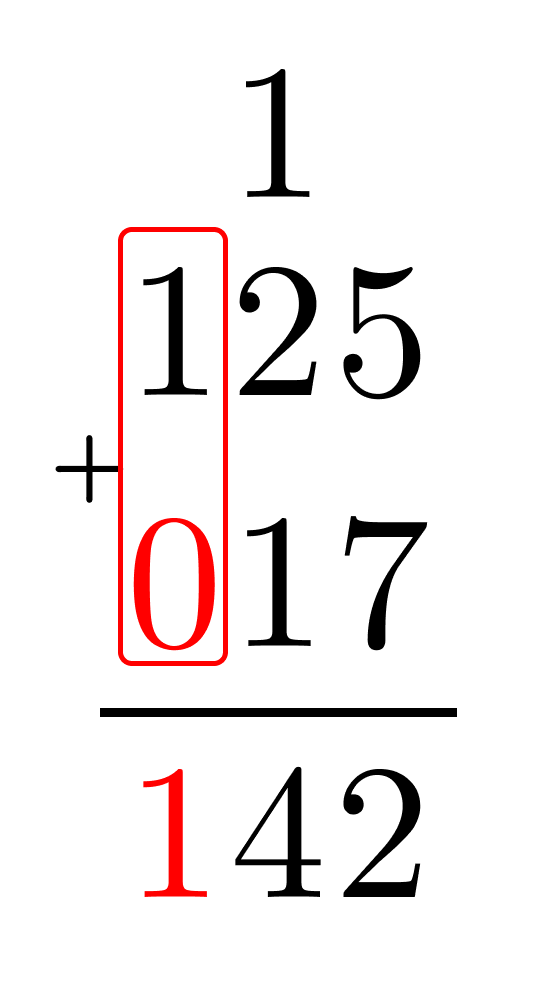
\includegraphics[width=0.25\linewidth]{imagens/soma_125_17_5.png}
        \label{fig:soma_125_17_5}
    \end{figure}

    Como não temos mais números para continuar nosso procedimento, o resultado será dado pelo número abaixo da linha.

    Portanto, a soma de \textbf{125} e \textbf{17} é \textbf{142}.
\end{exemplo}

Um último exemplo, passo à passo.

\begin{exemplo}
    Soma de 953 e 271:

    \begin{figure}[H]
        \centering
        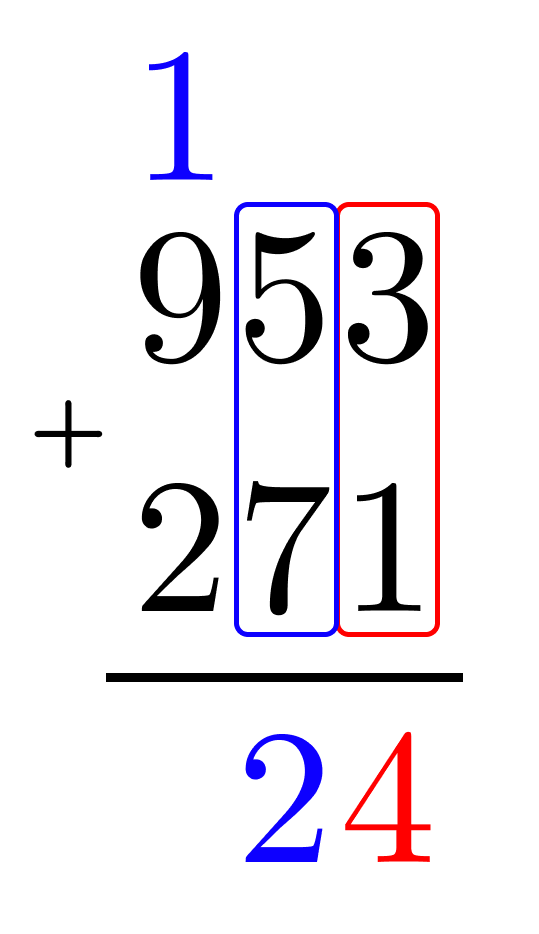
\includegraphics[width=0.25\linewidth]{imagens/soma_953_271_1.png}
        \label{fig:soma_953_271_1}
    \end{figure}

    Até aqui não temos nada de novo.

    \vspace{0.5cm}
    
    Agora, observe que o resultado da soma 1 + 9 + 2 = 12 teria que ser separada em ``1'' e ``2'', mas não temos mais números à esquerda para colocar o ``1'' em cima, certo? Então, simplesmente escrevemos o número 12 por inteiro na parte de baixo da linha.

    \begin{figure}[H]
        \centering
        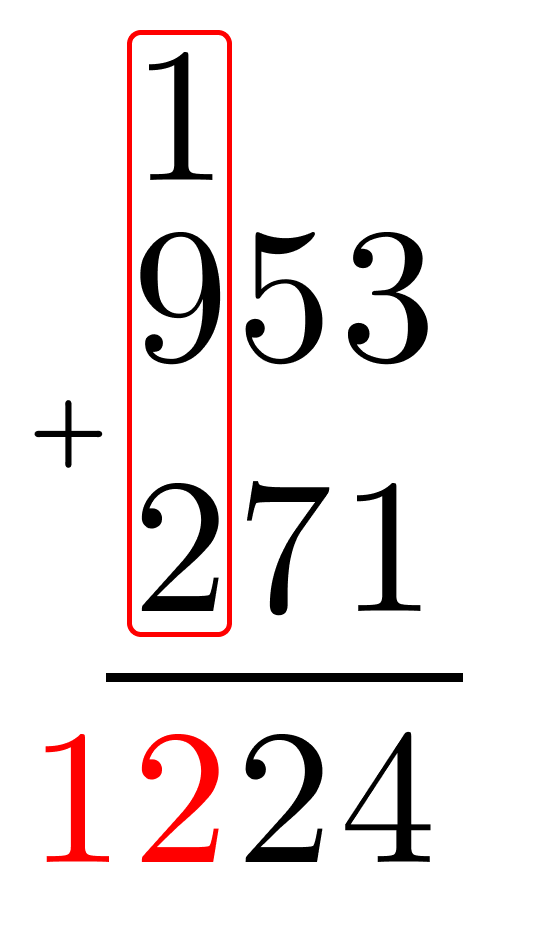
\includegraphics[width=0.25\linewidth]{imagens/soma_953_271_2.png}
        \label{fig:soma_953_271_2}
    \end{figure}

    Esgotados os números para nosso procedimento, paramos por aqui.

    Portanto, a soma de \textbf{953} e \textbf{271} é \textbf{1224}.
\end{exemplo}

A título de informação, vejamos mais três exemplos para fixar o procedimento, sem muitos comentários dessa vez.

\begin{exemplo}
    Soma de 1473 e 238.

    \begin{figure}[H]
        \centering
        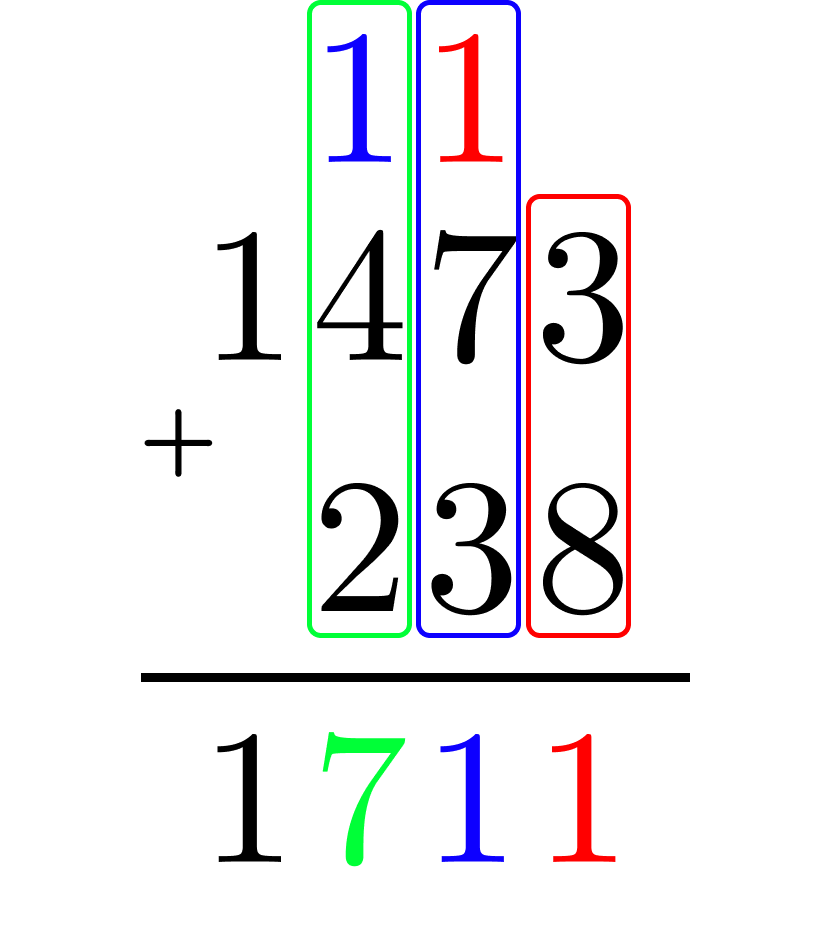
\includegraphics[width=0.35\linewidth]{imagens/soma_1473_238.png}
        \label{fig:soma_1473_238}
    \end{figure}

    Logo, a soma de \textbf{1473} e \textbf{238} é \textbf{1711}.
\end{exemplo}

\begin{exemplo}
    Soma de 117 e 1239.

    \vspace{0.5cm}

    Esse exemplo fica a título de curiosidade: e se colocássemos o número menor em cima ao invés do maior? 

    \begin{figure}[H]
        \centering
        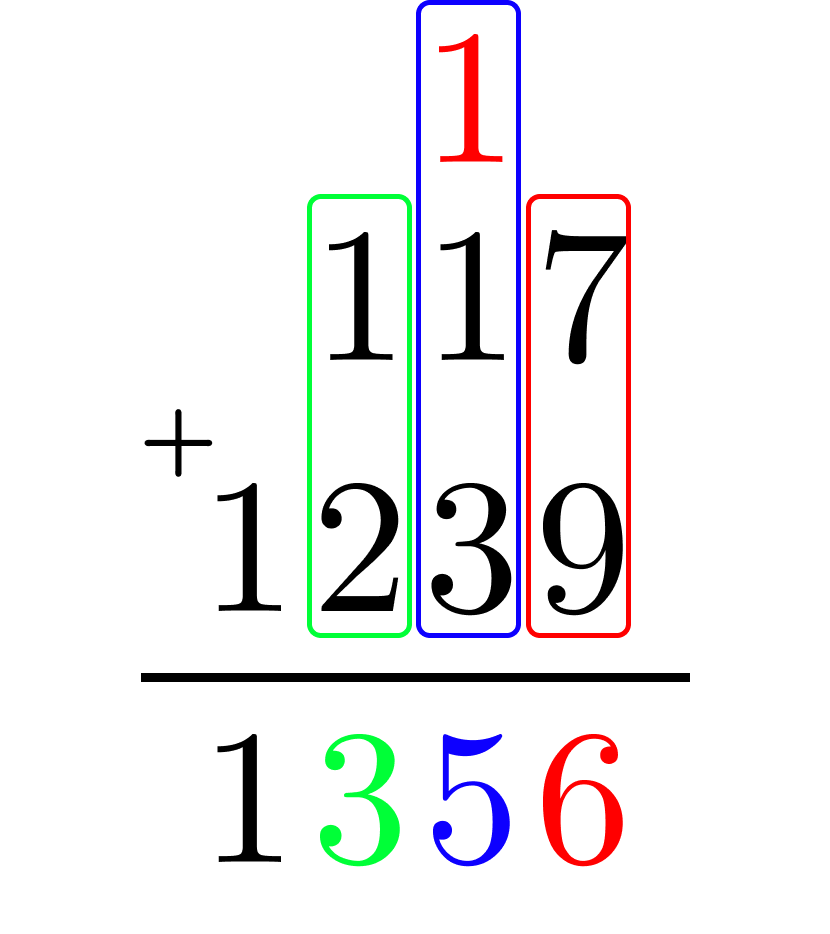
\includegraphics[width=0.35\linewidth]{imagens/soma_117_1239.png}
        \label{fig:soma_117_1239}
    \end{figure}

    Resposta: nada mudaria. E nem deveria, pois adição tem a propriedade comutativa. O importante é que as ordens/casas fiquem alinhadas, unidade abaixo de unidade, dezena abaixo de dezena etc.

    \vspace{0.5cm}  

    Logo, a soma de \textbf{117} e \textbf{1239} é \textbf{1356}.
\end{exemplo}

\begin{exemplo}
    Soma de 984 e 65.
    
    \begin{figure}[H]
        \centering
        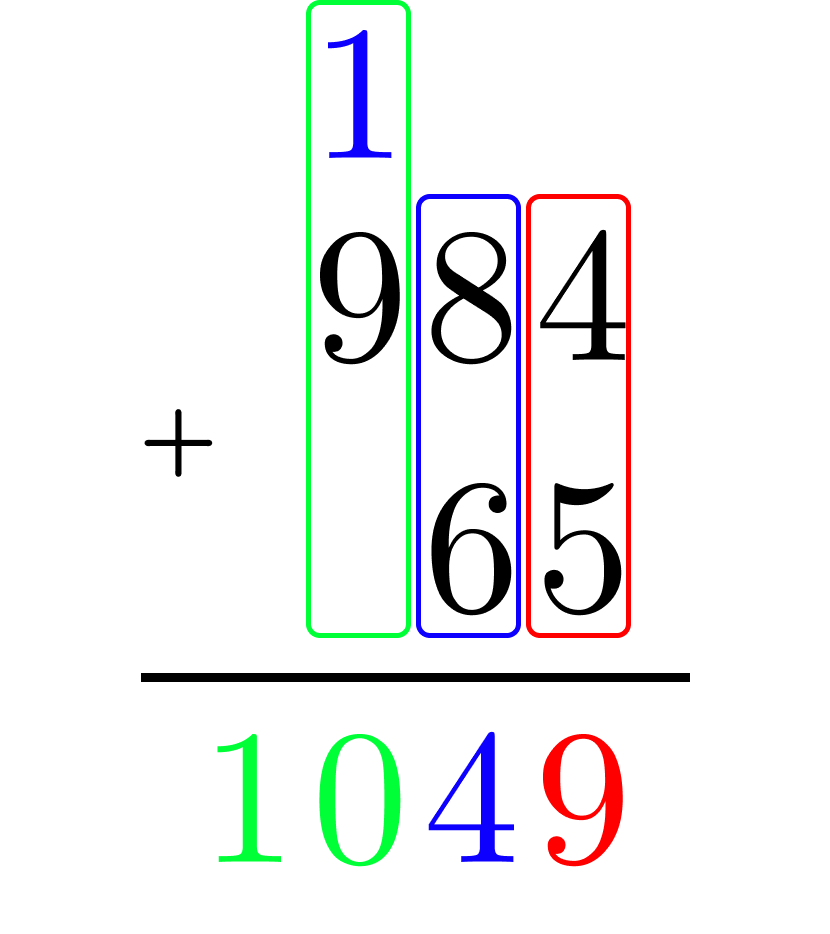
\includegraphics[width=0.35\linewidth]{imagens/soma_984_65.png}
        \label{fig:soma_984_65}
    \end{figure}

    Logo, a soma de \textbf{984} e \textbf{65} é \textbf{1049}.
\end{exemplo}


\newpage
\section{Subtração}

No caso da operação de subtração, podemos pensar nela de duas maneiras: 

\begin{enumerate}
    \item Como a diferença entre dois números positivos; ou seja, uma operação inversa da adição (que é a subtração que conhecemos no dia a dia);

    \begin{equation}
        A-B
    \end{equation}

    \item Ou como a soma entre um número positivo e outro negativo.

    \begin{equation}
        A+(-B)
    \end{equation}
\end{enumerate}

Essa segunda forma pode não parecer muito natural a princípio, mas é uma maneira interessante e bem útil de se analisar uma subtração. Além disso, ela nos inicia no estudo de uma nova classe de números: os negativos.

\subsection{Dispositivo Prático}

Como vimos na adição, também temos um procedimento similar para realizarmos uma subtração.

\begin{exemplo}
    Subtração de 16 e 15.

    A disposição dos números será a mesma: o maior em cima e o menor embaixo, de maneira que os algarismos de cada ordem (unidade e dezena) se encontrem (o “6 e 5” e “1 e 1”, no nosso exemplo).

    \begin{figure}[H]
        \centering
        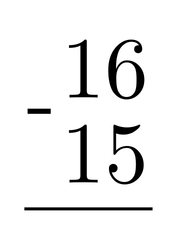
\includegraphics[width=0.2\linewidth]{imagens/sub_16_15_1.png}
        \label{fig:sub_16_15_1}
    \end{figure}

    Analisando os termos circulados, verificamos então se o algarismo de cima (6) é maior ou igual ao de baixo (5) para que possamos subtraí-los. Como 6 é maior que 5, efetuamos a subtração 6 – 5 = 1 e escrevemos o resultado abaixo da linha.

    \begin{figure}[H]
        \centering
        
\includegraphics[width=0.2\linewidth]{imagens/sub_16_15_2.png}
        \label{fig:sub_16_15_2}
    \end{figure}

    Passando para a esquerda, temos que o algarismo em cima (1) é igual ao de baixo (1), então efetuamos a subtração 1 – 1 = 0 e escrevemos o resultado abaixo da linha.

    \begin{figure}[H]
        \centering
        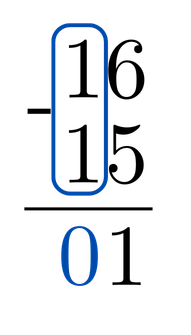
\includegraphics[width=0.2\linewidth]{imagens/sub_16_15_3.png}
        \label{fig:sub_16_15_3}
    \end{figure}

    Como não temos mais números para subtrair, o nosso procedimento se encerra aqui.

    \begin{figure}[H]
        \centering
        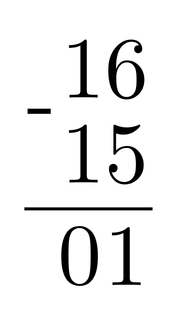
\includegraphics[width=0.2\linewidth]{imagens/sub_16_15_4.png}
        \label{fig:sub_16_15_4}
    \end{figure}
    
    Portanto, temos que o resultado de \textbf{16} menos \textbf{15} é \textbf{01} , ou simplesmente \textbf{1}.
\end{exemplo}

Vamos complicar um pouco.

\begin{exemplo}
    Subtração de 125 e 17:

    Perceba que, assim como na adição, o importante é os algarismos das unidades se encontrarem (5 e 7, no exemplo)

    \begin{figure}[H]
        \centering
        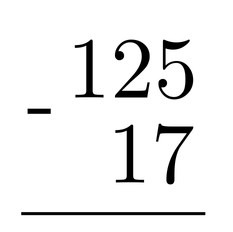
\includegraphics[width=0.25\linewidth]{imagens/sub_125_17_1.png}
        \label{fig:sub_125_17_1}
    \end{figure}

    E, novamente, podemos considerar o 17 como 017, para facilitar a visualização. Nesse caso, temos uma novidade: o número de cima (5) é menor que o de baixo (7). O procedimento nos diz que em casos assim, precisamos fazer o seguinte:

    \begin{enumerate}
        \item ``Roubar'' uma dezena do algarismo da esquerda, 2, deixando-o com o novo valor de 1, pois: 2 – 1 = 1;
        \item Esse valor de 1 que subtraímos, correspondendo à 1 dezena, vamos transformá-lo em unidades adicionando um 0 a sua direita, transformando-o em 10. (perceba que não estamos somando o zero, apenas escrevendo-o a direita de 1);
        \item Agora, somamos os dois números, 10 + 5, totalizando 15.
    \end{enumerate}

    Então:

    \begin{figure}[H]
        \centering
        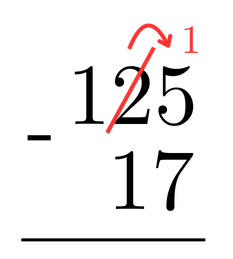
\includegraphics[width=0.25\linewidth]{imagens/sub_125_17_2.png}
        \label{fig:sub_125_17_2}
    \end{figure}

    Dessa maneira, temos que o número de cima, 15, é maior que o de baixo, 7. Então podemos efetuar nossa subtração, 15 – 7 = 8, e escrevemos o resultado abaixo da linha.

    \begin{figure}[H]
        \centering
        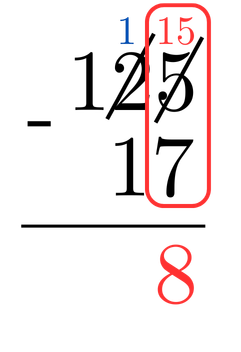
\includegraphics[width=0.25\linewidth]{imagens/sub_125_17_3.png}
        \label{fig:sub_125_17_3}
    \end{figure}

    Agora, passamos para a esquerda e notamos que o número de cima, no caso o 1, pois o número 2 não existe mais, já é igual ao de baixo (1). Então, efetuamos a subtração 1 – 1 = 0, e escrevemos o resultado abaixo da linha.

    \begin{figure}[H]
        \centering
        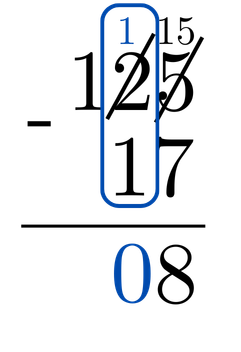
\includegraphics[width=0.25\linewidth]{imagens/sub_125_17_4.png}
        \label{fig:sub_125_17_4}
    \end{figure}

    Lembrando que podemos tratar o “17” como “017” para uma melhor visualização. Então, nossa subtração será: 1 – 0 = 1.

    \begin{figure}[H]
        \centering
        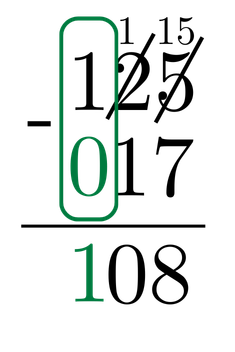
\includegraphics[width=0.25\linewidth]{imagens/sub_125_17_5.png}
        \label{fig:sub_125_17_5}
    \end{figure}

    Como não temos mais números à esquerda, nosso procedimento se encerra aqui. Sabemos, então, que o resultado de \textbf{125} menos \textbf{17} é \textbf{108}.

    \begin{figure}[H]
        \centering
        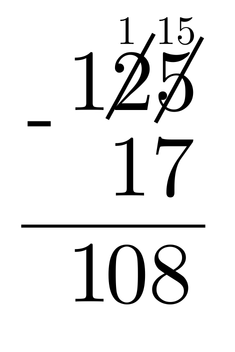
\includegraphics[width=0.25\linewidth]{imagens/sub_125_17_6.png}
        \label{fig:sub_125_17_6}
    \end{figure}

\end{exemplo}

A tentativa de explicar o dispositivo prático de subtração, sem as nomenclaturas e ferramentas corretas, torna o processo mais confuso e difícil. Mas, o segredo é sempre ``roubar'' ordens da esquerda para completarmos os algarismos que precisarem. Com a prática, ficará mais claro que esse desenvolvimento é relativamente fácil.

Vejamos mais um exemplo para fixar o conceito.

\begin{exemplo}
    Subtração de 953 e 274:

    \begin{figure}[H]
        \centering
        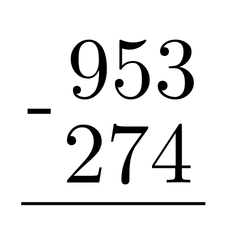
\includegraphics[width=0.25\linewidth]{imagens/sub_953_274_1.png}
        \label{fig:sub_953_274_1}
    \end{figure}

    Nossa primeira subtração da direita é entre 3 e 4. Como 3 é menor que 4, temos que pegar uma dezena emprestada do nosso algarismo das dezenas ao lado, 5, como vimos no exemplo anterior.

    \begin{figure}[H]
        \centering
        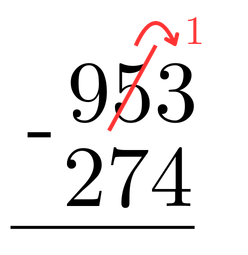
\includegraphics[width=0.25\linewidth]{imagens/sub_953_274_2.png}
        \label{fig:sub_953_274_2}
    \end{figure}

    Dessa maneira, o que era 3 se torna 13 (10+3), e o que era 5 se torna 4. Agora, podemos seguir com a subtração de 13 – 4 = 9.

    \begin{figure}[H]
        \centering
        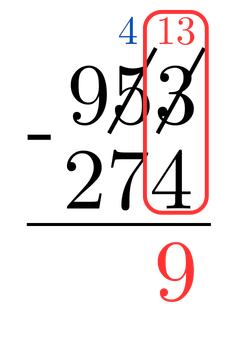
\includegraphics[width=0.25\linewidth]{imagens/sub_953_274_3.png}
        \label{fig:sub_953_274_3}
    \end{figure}

    Continuando, encontramos agora uma subtração de 4 (o antigo 5) por 7. Como 4 é menor do que 7, temos que pegar uma centena emprestada do nosso novo número à esquerda: 9. Essa centena ~e ent"ao convertida em 10 dezenas, de modo semelhante ao que fizemos no caso das dezenas e unidades no exemplo anterior.

    Assim, o 4 se torna 14 (10+4) e o 9 passa a ser 8. 

    \begin{figure}[H]
        \centering
        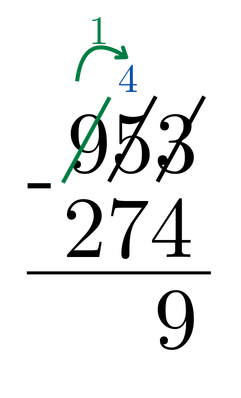
\includegraphics[width=0.25\linewidth]{imagens/sub_953_274_4.png}
        \label{fig:sub_953_274_4}
    \end{figure}

    Como 14 é maior do que 7, podemos continuar nossa subtraçãoÇ 14 – 7 = 7.

    \begin{figure}[H]
        \centering
        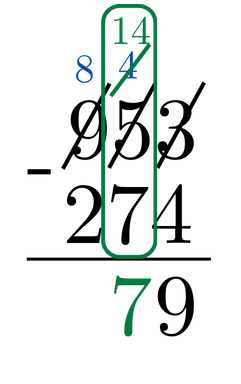
\includegraphics[width=0.25\linewidth]{imagens/sub_953_274_5.png}
        \label{fig:sub_953_274_5}
    \end{figure}

    Chegamos agora ao último número da esquerda 8 (antigo 9). Podemos ver que 8 já é maior do que 2, então podemos simplesmente efetuar a subtração 8 – 2 = 6.

    \begin{figure}[H]
        \centering
        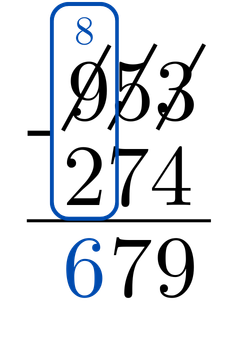
\includegraphics[width=0.25\linewidth]{imagens/sub_953_274_6.png}
        \label{fig:sub_953_274_6}
    \end{figure}

    Como não temos mais números, chegamos ao final do nosso procedimento, apõs um longo processo. O resultado de \textbf{953} menos \textbf{274} é \textbf{679}.

    \begin{figure}[H]
        \centering
        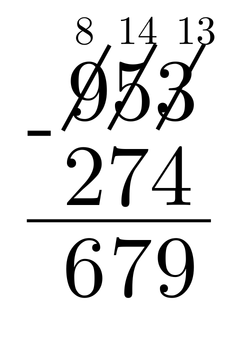
\includegraphics[width=0.25\linewidth]{imagens/sub_953_274_7.png}
        \label{fig:sub_953_274_7}
    \end{figure}
\end{exemplo}

Agora podemos começar a trabalhar com exemplos que envolvem a operação de subtração.

\begin{exemplo}
    Ladrão de coxinhas.

    Lorena tem 10 coxinhas em sua merendeira. Matheus, um infeliz amante de coxinhas, resolve roubar 4 do estoque de Lorena. Quantos salgadinhos sobram com Lorena?\\

    De 10 coxinhas, tiram-se 4, então temos: \\

    10 - 4 = 6 coxinhas restantes \\
 
    \textcolor{red}{Observação}: Neste exemplo, não faz sentido interpretar a subtração como \(10+(-4)\),pois não conseguimos representar concretamente a ideia de -4 coxinhas.
\end{exemplo}

\subsection{Propriedades}

A vantagem de pensarmos a subtração como uma soma é que podemos utilizar todas as propriedades da adição (elemento zero, comutativa, associativa). Veja:

\begin{tcolorbox}[title = Comutativa]
    \begin{equation}
        A-B \Rightarrow A+(-B) \Rightarrow -B+A
    \end{equation}
\end{tcolorbox}

Por exemplo:

\begin{equation}
    -2+3=+3-2=1
\end{equation}

\begin{tcolorbox}[title = Associativa]
    \begin{equation}
        (A - B) + C \Rightarrow [ A + (-B) ] + C 
    \end{equation}

    \begin{equation}
        \Rightarrow A + [ (-B) + C ] \Rightarrow A + (C - B)
    \end{equation}
\end{tcolorbox}

Por exemplo:

\begin{equation}
    (2-3)+4=2+(4-3)=3
\end{equation}

E assim por diante. 

\newpage
\section{Multiplicação}

Podemos analisar a multiplicação como uma soma repetida de números, sejam positivos ou negativos.

\begin{equation}
    A = 5 \times B=B+B+B+B+B
\end{equation}

Então, dizemos que \textbf{A} é igual a \textbf{5} vezes o número \textbf{B}, pois B é somado cinco vezes. O resultado de uma multiplicação é chamado de \textbf{produto}.

A \textbf{tabuada} é uma ferramenta importante para nos ajudar a realizar o processo de multiplicação, a qual infelizmente nós devemos decorar e/ou utilizar como consulta.

%\begin{tcolorbox}[title=\textbf{Tabuada}]
    
    \begin{table}[H]
        \centering
        \begin{tabular}{|c|c|c|c|c|c|c|c|c|c|c|}
        \hline
            $\times$ & \textbf{1} & \textbf{2} & \textbf{3} & \textbf{4} & \textbf{5} & \textbf{6} & \textbf{7} & \textbf{8} & \textbf{9} & \textbf{10}\\  \hline
             \textbf{1} & 1 & 2 & 3 & 4 & 5 & 6 & 7 & 8 & 9 & 10\\ \hline
             \textbf{2} & 2 & 4 & 6 & 8 & 10 & 12 & 14 & 16 & 18 & 20\\ \hline
             \textbf{3} & 3 & 6 & 9 & 12 & 15 & 18 & 21 & 24 & 27 & 30\\ \hline
             \textbf{4} & 4 & 8 & 12 & 16 & 20 & 24 & 28 & 32 & 36 & 40\\ \hline
             \textbf{5} & 5 & 10 & 15 & 20 & 30 & 30 & 35 & 40 & 45 & 50\\ \hline
             \textbf{6} & 6 & 12 & 18 & 24 & 35 & 36 & 42 & 48 & 54 & 60\\ \hline
             \textbf{7} & 7 & 14 & 21 & 28 & 40 & 42 & 49 & 56 & 63 & 70\\ \hline
             \textbf{8} & 8 & 16 & 24 & 32 & 45 & 48 & 56 & 64 & 72 & 80\\ \hline
             \textbf{9} & 9 & 18 & 27 & 36 & 50 & 54 & 63 & 72 & 81 & 90\\ \hline
             \textbf{10} & 10 & 20 & 30 & 40 & 50 & 60 & 70 & 80 & 90 & 100\\
        \hline
        \end{tabular}
        \caption{Tabuada de 1 a 10}
        \label{tab:tabuada_1_a_10}
    \end{table}
%\end{tcolorbox}

\begin{exemplo}
    Multiplicação de dois números positivos:

    \begin{equation}
        2 \times 5 = 10
    \end{equation}

    O que é equivalente de somar o número \textbf{2} por cinco vezes:

    \begin{equation}
        2+2+2+2+2 = 10
    \end{equation}

    Ou, somar o número \textbf{5} duas vezes:

    \begin{equation}
        5+5=10
    \end{equation}

    Perceba que o número \textbf{10} pode ser escrito como a multiplicação de \textbf{2} por \textbf{5}, que é o equivalente a soma repetida de cinco termos \textbf{2} ou a soma de dois termos \textbf{5}.
\end{exemplo}

\textcolor{red}{Observação}: a partir do exemplo anterior, já fica suspeito que a multiplicação talvez tenha uma propriedade comutativa. Será? Reflita a respeito (\textit{spoiler}: sim).

\begin{exemplo}
    Multiplicação de um número positivo por outro negativo:

    \begin{equation}
        4 \times (-2) = (-2)+(-2)+(-2)+(-2) = -8 
    \end{equation}

    Ou, podemos entender como:

    \begin{equation}
        2 \times (-4) = (-4) + (-4) = -8
    \end{equation}
\end{exemplo}

Observe que no segundo exemplo estamos usando a noção de subtração como uma soma de números negativos. Na prática, se torna uma subtração de vários termos repetidos, como vimos no tópico anterior. 

Podemos fazer vários tipos de multiplicações diferentes: positivo com positivo, negativo com positivo, positivo com negativo e negativo com negativo. Então, vamos aproveitar o nosso conhecimento de multiplicação e números negativos para elaborarmos um método para identificar mais facilmente o sinal resultado desses tipos de multiplicações. Qual será o sinal que ``sobra'' no final de uma multiplicação: positivo ou negativo?

\subsection{Regra de Sinais}

Queremos descobrir qual é o sinal resultante das seguintes multiplicações:

\begin{itemize}
    \item número positivo (+) e número positivo (+); 
    \item número positivo (+) e número negativo (-); 
    \item número negativo (-) e número positivo (+); 
    \item número negativo (-) e número negativo (-).
\end{itemize}

Para isso, vamos pensar em uma analogia, sendo:

\begin{enumerate}
    \item \textbf{Positivo} \(\times\) \textbf{Positivo}: (+) \(\times\) (+).
    
    \(\rightarrow\) o amigo (+) de um amigo (+) é também meu amigo (+). 

    \textbf{Portanto}: (+) \(\times\) (+) = (+)

    \item \textbf{Positivo} \(\times\) \textbf{Negativo}: (+) \(\times\) (-).
    
    \(\rightarrow\) o amigo (+) de um inimigo (-) é também meu inimigo (-). 

    \textbf{Portanto}: (+) \(\times\) (-) = (-)

    \item \textbf{Negativo} \(\times\) \textbf{Positivo}: (-) \(\times\) (+).
    
    \(\rightarrow\) o inimigo (-) de um amigo (+) é também meu inimigo (-). 

    \textbf{Portanto}: (-) \(\times\) (+) = (-)

    \item \textbf{Negativo} \(\times\) \textbf{Negativo}: (-) \(\times\) (-).
    
    \(\rightarrow\) o inimigo (-) de um inimigo (-) é meu amigo (+). 

    \textbf{Portanto}: (-) \(\times\) (-) = (+)

    Imagine que nós  viramos amigos momentaneamente contra um inimigo em comum (apesar de haver uma certa controvérsia nisso).
\end{enumerate}

\textcolor{red}{Observação}: Apesar de simples e deselegante, esse método pode ser útil durante a resolução de questões, principalmente em provas.

Vejamos um exemplo:

\begin{exemplo}
    Multiplicações entre números com o mesmo sinal e/ou com sinais diferentes.
    
    \begin{enumerate}
        \item (+2) \(\times\) (+3) = +6
        \item (+2) \(\times\) (-3) = -6
        \item (-2) \(\times\) (+3) = -6
        \item (-2) \(\times\) (-3) = +6
    \end{enumerate}
    
\end{exemplo}


\subsection{Primeira Lei da Multiplicação}

O produto do número zero por qualquer outro número ‘N’ é igual a zero.

\begin{tcolorbox}[title = Primeira Lei da Multiplicação]
    Seja N um número qualquer, então:
    \begin{equation}
        0 \times N = 0
    \end{equation}
\end{tcolorbox}


Podemos pensar que é como ``somar o mesmo número zero vezes'', ou seja, nenhuma vez.

\subsection{Segunda Lei da Multiplicação}

Ou \textbf{Lei do Elemento Neutro}, tem a mesma ideia de ``elemento neutro'' que vimos em adição: um número que multiplicado por outro e não afeta o resultado. A multiplicação do número 1 por qualquer outro número ‘N’ não altera o valor desse número (N). Por isso 1 é dito Elemento Neutro, sua presença no produto não altera o resultado.

\begin{tcolorbox}[title = Segunda Lei da Multiplicação]
    Seja N um número qualquer, então:
    \begin{equation}
        1 \times N = N
    \end{equation}
\end{tcolorbox}

\begin{exemplo}
    Alguns exemplos:

    \begin{enumerate}
        \item \(1 \times 5 = 5\)
        \item \(1 \times 3 = 3\)
        \item \(1 \times1 \times1 \times1 \times1 \times1 \times 5 = 5\)
    \end{enumerate}
\end{exemplo}

\subsection{Terceira Lei da Multiplicação}

Também chamada de \textbf{distributiva}, ou ``chuverinho'', é toda multiplicação na qual um termo fora dos parênteses multiplica uma soma de números dentro dos parênteses. Perceba que teremos 2 casos interessantes: 

\begin{enumerate}
    \item \textbf{Quando o número de fora dos parênteses estiver sozinho}:

    \begin{equation}
        A\times(B+C)=A\times B+A \times C
    \end{equation}

    Observe que o termo independente A é multiplicado por cada um dos termos da soma (B + C).

    \begin{exemplo}
        Considere a seguinte multiplicação:

        \begin{equation}
            3\times(2+4)= 3 \times 2 + 3 \times 4
        \end{equation}

        \begin{equation}
            =6+12=18
        \end{equation}

        Note que o número 3 está multiplicando cada um dos termos da soma. Outra maneira de realizar essa conta, seria primeiro somar os valores dentro do parênteses: $3\times(2 + 4)$ \(\Rightarrow\) $3\times(6)$ \(\Rightarrow\) $18$. \\

        Perceba que o resultado é o mesmo de quando somamos os valores dentro dos parênteses antes de multiplicar pelo número de fora.
    \end{exemplo}

    \item \textbf{Quando o termo de fora dos parênteses é também uma soma de 2 ou mais números}:

    \begin{equation}
        (\textcolor{red}{A} + \textcolor{red}{B})\times(C + D) = \textcolor{red}{A}\times C + \textcolor{red}{A}\times D + \textcolor{red}{B}\times C + \textcolor{red}{B}\times D 
    \end{equation}

    Observe que os elementos da primeira soma (A + B) são multiplicados cada um pelos elementos da segunda soma (C + D). Temos A multiplicado pelo primeiro termo C e em seguida por D e o mesmo acontece com B (B\(\times\)C + B\(\times\)D).

    \begin{exemplo}
        Considere a seguinte multiplicação:

        \begin{equation}
            (3 + 5)\times(2 + 4) = 3\times2 + 3\times4 + 5\times2 + 5\times4 
        \end{equation}

        \begin{equation}
            = 6 + 12 + 10 + 20 = \textbf{48}
        \end{equation}

        Note que o número 3 está multiplicando cada um dos termos da soma (2 + 4) e o mesmo ocorre com o número 5.\\
        
        Uma maneira equivalente de tratarmos o exemplo é realizarmos a soma antes de realizarmos a multiplicação:

        \begin{equation}
             (3 + 5)\times(2 + 4) = (8)\times(6) = \textbf{48}
        \end{equation}
    \end{exemplo}    
\end{enumerate}

\subsection{Propriedade comutativa}

A propriedade comutativa afirma que alterar a ordem de multiplicação dos fatores não altera o produto (``\textit{a ordem dos fatores não altera o produto''}).

\begin{equation}
    A\times B=B\times A
\end{equation}

\begin{exemplo}
    Considere as seguintes multiplicações:

    \begin{equation}
        2\times 3= 6
    \end{equation}

    \begin{equation}
        3\times 2= 6
    \end{equation}

    Observe que o resultado é igual a 6, independente da ordem dos fatores (2\(\times\)3 = 6 ou 3\(\times\)2 = 6).
\end{exemplo}

\subsection{Propriedade associativa}

Quando temos mais de dois números, essa propriedade afirma que a ordem em que os números são multiplicados não afeta o resultado. 

\begin{equation}
    (A\times B)\times C=A \times (B \times C)
\end{equation}

\begin{exemplo}
    Considere as seguintes multiplicações:

    \begin{equation}
        (2\times3)\times4=(6)\times4=24
    \end{equation}
    
    ou
    
    \begin{equation}
        2\times(3\times4)=2\times(12)=24
    \end{equation}

    Em ambos os casos o resultado final é o mesmo. E deve ser.
\end{exemplo}

\subsection{Dispositivo Prático}

O dispositivo prático para efetuarmos multiplicações é de certa forma parecido com o de adição. Perceba que para produtos entre número menores que “10” (0 a 9) esse dispositivo não terá muita utilidade, nesse caso devemos recorrer à boa e velha tabuada. Vejamos alguns exemplos numéricos já de início.

\begin{exemplo}

    Para iniciarmos a discussão sobre o dispositivo prático, primeiro vamos começar com um exemplo que não seria necessário utilizá-lo (pois já saberíamos fazer somente com a tabuada), mas que vai nos ajudar visualmente.

    \vspace{0.5cm}

    Primeiro, temos que colocar um número em cima do outro (similar ao que fizemos na adição), colocar um símbolo de multiplicação à esquerda (x) e traçar uma linha abaixo para representarmos os resultados.
    
    \begin{figure}[H]
        \centering
        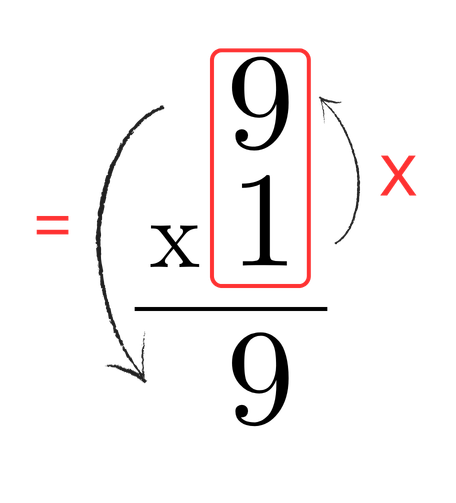
\includegraphics[width=0.3\linewidth]{imagens/mult_1_9.png}
        \label{fig:mult_1_9}
    \end{figure}
    
    Nesse caso só temos esses dois únicos números para operar, então multiplicamos o de baixo pelo de cima e o resultado é escrito abaixo da linha. 

    \vspace{0.5cm}

    E aqui não temos nenhuma novidade, pois já sabíamos que o produto de um número por 1 é ele mesmo.
\end{exemplo}

De regra geral, costumamos escrever o maior número por cima e o menor número por baixo (principalmente com 2 ou mais algarismos) mais por uma questão de visualização e facilidade. A ordem inversa não faria diferença, pois multiplicação é comutativa, não é mesmo?

Outra ``regra'' que já vamos quebrar no próxima exemplo, é que a abaixo de cada algarismo ''só é permitido´´ um único número. Vejamos como isso funcionaria.

\begin{exemplo}

    Vejamos agora mais um exemplo em que somente a tabuada seria o suficiente para encontrarmos o produto.

    \begin{figure}[H]
        \centering
        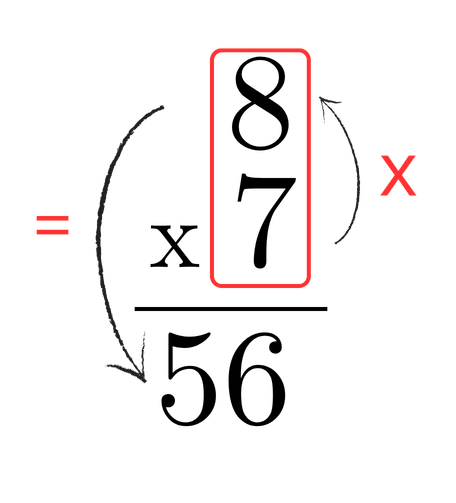
\includegraphics[width=0.3\linewidth]{imagens/mult_7_8.png}
        \label{fig:mult_7_8}
    \end{figure}

    E aqui novamente repetimos o procedimento de colocar o menor número em baixo, o maior em cima, o sinal de multiplicação e a linha que delimita os nossos cálculos.

    \vspace{0.5cm}

    A ``regra'' que estamos quebrando aqui é o fato de que só poderíamos colocar o algarismo 6 abaixo do 7, mas como não existem outras operações a serem realizadas, simplesmente colocamos o resultado final da última multiplicação (como também havíamos feita para soma). 

    \vspace{0.5cm}

    Ou também podemos pensar o seguinte: abaixo do algarismo 7 realmente só existe o 6, e as outras casas à esquerda estão livres para os demais ocuparem sem problema (já que não teria nada acima deles)
\end{exemplo}

Vejamos agora um exemplo mais interessante que vai dar significado para o nosso dispositivo prático, quando um ou mais dos números possuírem mais algarismos.

\begin{exemplo}

    Ainda sim seria um exemplo que poderíamos pensar em ``tabuada'' do 11, mas vamos ver como ficaria no nosso dispositivo.

    \vspace{0.5cm}

    Primeiramente colocamos o menor número por baixo, que possui somente o algarismo das unidades, e o maior por cima com o algarismo das unidades se encontrando.

    \begin{figure}[H]
        \centering
        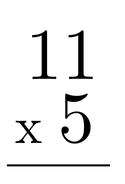
\includegraphics[width=0.16\linewidth]{imagens/mult_5_11_1.png}
        \label{fig:mult_5_11_1}
    \end{figure}

    Nada de novo até aqui. Mas agora, diferente da adição, escolhemos o primeiro algarismo de baixo (que nesse caso vai ser só o 5 mesmo) e multiplicamos por todos os de cima da direita para esquerda, veja:

    \begin{figure}[H]
        \centering
        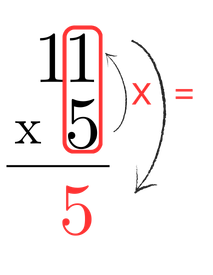
\includegraphics[width=0.28\linewidth]{imagens/mult_5_11_2.png}
        \label{fig:mult_5_11_2}
    \end{figure}

    A primeira multiplicação que temos que realizar é 5 por 1, que daí vamos pegar da nossa tabuada como resultado o próprio 5. Adicionamos ele abaixo da linha (em vermelho) e continuamos:

    \begin{figure}[H]
        \centering
        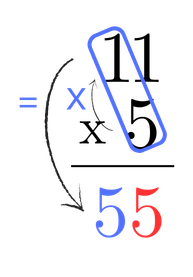
\includegraphics[width=0.28\linewidth]{imagens/mult_5_11_3.png}
        \label{fig:mult_5_11_3}
    \end{figure}

    Agora vamos multiplicar o 5 pelo algarismo 1 ``novamente'', só que agora com o que está na casa das dezenas. Nosso resultado (em azul) é adicionado abaixo da linha e paramos por aqui, obtendo o resultado final 55:

    \begin{figure}[H]
        \centering
        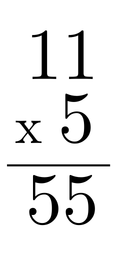
\includegraphics[width=0.17\linewidth]{imagens/mult_5_11_4.png}
        \label{fig:mult_5_11_4}
    \end{figure}

    Que poderíamos continuar multiplicando caso houvessem mais algarismos nas casas das centenas etc.
\end{exemplo}

Um último exemplo nessa linha para que o(a) estudante acredite que esse processo pode continuar infinitamente.

\begin{exemplo}
    Considere a multiplicação entre 3 e 120. Menor em baixo, maior em cima, linha horizontal pra dividir a brincadeira.

    \begin{figure}[H]
        \centering        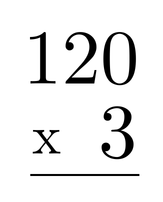
\includegraphics[width=0.2\linewidth]{imagens/mult_3_120_1.png}
        \label{fig:mult_3_120_1}
    \end{figure}

    Como só temos o algarismo/número 3 na parte de baixo, devemos multiplicar ele por todos outros de cima (da direita para esquerda), começando pelo 0:

    \begin{figure}[H]
        \centering
        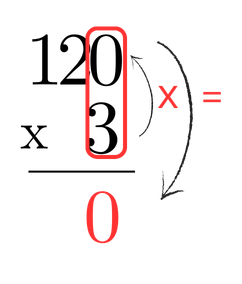
\includegraphics[width=0.3\linewidth]{imagens/mult_3_120_2.png}
        \label{fig:multi_3_120_2}
    \end{figure}

    Vamos repetir o processo até chegar no último algarismo da esquerda:

    \begin{figure}[H]
        \centering
        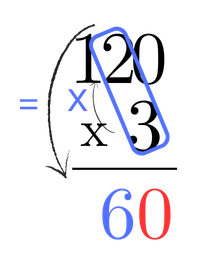
\includegraphics[width=0.28\linewidth]{imagens/mult_3_120_3.png}
        \label{fig:multi_3_120_3}
    \end{figure}

    \begin{figure}[H]
        \centering
        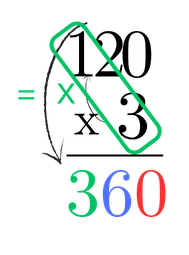
\includegraphics[width=0.28\linewidth]{imagens/mult_3_120_4.png}
        \label{fig:multi_3_120_4}
    \end{figure}

    E finalizamos nosso processo novamente, quando acabam os algarismos para multiplicarmos, ficando com o resultado de 360:

    \begin{figure}[H]
        \centering
        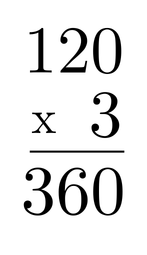
\includegraphics[width=0.22\linewidth]{imagens/mult_3_120_5.png}
        \label{fig:multi_3_120_5}
    \end{figure}
\end{exemplo}

E agora um último exemplo com somente um algarismo na parte de baixo da multiplicação, que vai introduzir uma coisa ``nova'' no dispositivo.

\begin{exemplo}

    Considere a multiplicação de 7 por 13. 
    
    \begin{figure}[H]
        \centering
        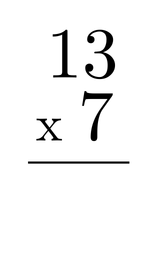
\includegraphics[width=0.23\linewidth]{imagens/mult_7_13_1.png}
        \label{fig:mult_7_13_1}
    \end{figure}

    Realizamos a primeira multiplicação de 7 por 3, que dá 21. E aqui temos a novidade para o dispositivo prático da multiplicação. 

    \begin{figure}[H]
        \centering
        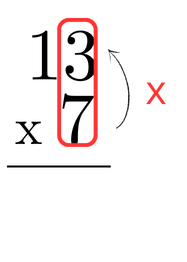
\includegraphics[width=0.28\linewidth]{imagens/mult_7_13_2.png}
        \label{fig:mult_7_13_2}
    \end{figure}

    Da mesma forma como vimos na adição, quando uma soma (produto nesse caso) de dois algarismos dava 10 ou mais, colocávamos abaixo da linha somente o algarismo das unidades e os demais (nesse caso sobra somente um) levamos para parte superior do próximo algarismo ``de cima''. Veja:

    \begin{figure}[H]
        \centering
        
\includegraphics[width=0.22\linewidth]{imagens/mult_7_13_3.png}
        \label{fig:mult_7_13_3}
    \end{figure}

    E aqui temos algo \textbf{importante}: quando realizarmos a próxima multiplicação, entre 7 e 1, ignoramos o número 2 lá em cima. Só depois que encontrarmos o produto de 7 e 1 daí somamos o 2.

    \begin{figure}[H]
        \centering
        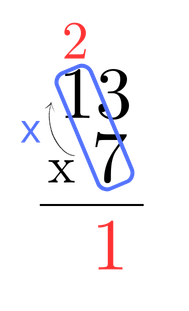
\includegraphics[width=0.25\linewidth]{imagens/mult_7_13_4.png}
        \label{fig:mult_7_13_4}
    \end{figure}

    Que nesse caso será: \(7\times1+2=9\).

    \begin{figure}[H]
        \centering
        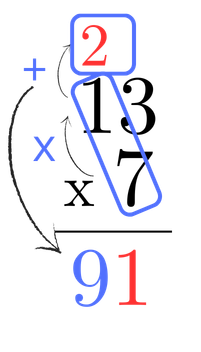
\includegraphics[width=0.25\linewidth]{imagens/mult_7_13_5.png}
        \label{fig:mult_7_13_5}
    \end{figure}

    E por fim ficamos com o nosso resultado, 91.

    \begin{figure}[H]
        \centering
        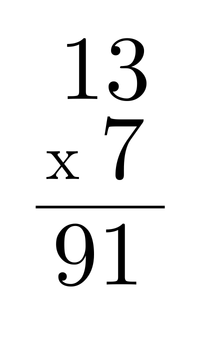
\includegraphics[width=0.20\linewidth]{imagens/mult_7_13_6.png}
        \label{fig:mult_7_13_6}
    \end{figure}
\end{exemplo}

Nesse momento o(a) aluno(a) deve estar pensando: ``Ah, só isso? Achei que seria algo interessante pra merecer tanta atenção''. E nesse momento a infelicidade de proferir esses pensamentos se manifesta. Que tal adicionarmos mais algarismos na parte de baixo também?

\begin{exemplo}

    Considere a multiplicação entre 36 e 57. Na verdade o processo é bem similar, com uma pequena diferença que veremos logo mais.

    \begin{figure}[H]
        \centering
        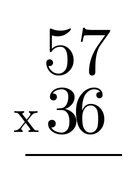
\includegraphics[width=0.2\linewidth]{imagens/multi_36_57_1.png}
        \label{fig:multi_36_57_1}
    \end{figure}

    A primeira parte é exatamente como estávamos resolvendo até então, pegamos o primeiro algarismo da parte de baixo (6) e multiplicamos por todos na parte de cima:

    \begin{figure}[H]
        \centering
        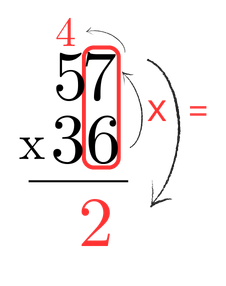
\includegraphics[width=0.3\linewidth]{imagens/multi_36_57_2.png}
        \label{fig:multi_36_57_2}
    \end{figure}

    \begin{figure}[H]
        \centering
        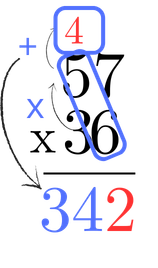
\includegraphics[width=0.24\linewidth]{imagens/multi_36_57_3.png}
        \label{fig:multi_36_57_3}
    \end{figure}

    E até aqui vimos alguns exemplos de como resolver já. A partir de agora, temos que pegar o próximo algarismo de baixo (3) e multiplicar por todos de cima da mesma maneira. Porém, vamos colocar os resultados \textbf{abaixo} dos resultados anteriores e \textbf{deslocados um algarismo para esquerda}. 

    \begin{figure}[H]
        \centering
        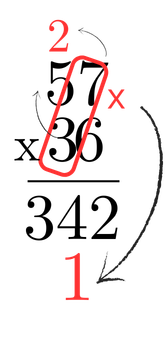
\includegraphics[width=0.24\linewidth]{imagens/multi_36_57_4.png}
        \label{fig:multi_36_57_4}
    \end{figure}

    E aqui já podemos ver a diferença: ao invés do algarismo 1 ficar abaixo do 2, ele fica deslocado uma casa para esquerda, abaixo do 4. Mas o restante do processo é exatamente o mesmo.

    \begin{figure}[H]
        \centering
        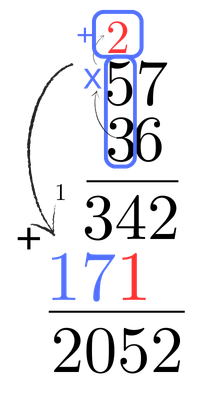
\includegraphics[width=0.28\linewidth]{imagens/multi_36_57_5.png}
        \label{fig:multi_36_57_5}
    \end{figure}

    E uma vez que terminamos de multiplicar por todos de cima, somamos o primeiro resultado (\(342\)) com o segundo resultado (\(171\)), obtendo \(2052\) como resultado.

    \begin{figure}[H]
        \centering
        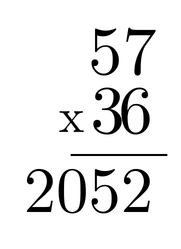
\includegraphics[width=0.24\linewidth]{imagens/multi_36_57_6.png}
        \label{fig:multi_36_57_6}
    \end{figure}
\end{exemplo}

\begin{exemplo}
    Considere a multiplicação de 36 por 421. Vamos executar os passos vistos anteriormente.

    \begin{figure}[H]
        \centering
        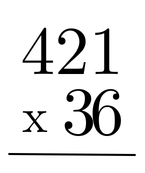
\includegraphics[width=0.18\linewidth]{imagens/mult_36_421_1.png}
        \label{fig:multi_36_421_1}
    \end{figure}

    \begin{figure}[H]
        \centering
        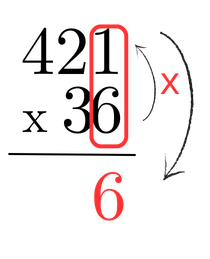
\includegraphics[width=0.25\linewidth]{imagens/mult_36_421_2.png}
        \label{fig:multi_36_421_2}
    \end{figure}

    \begin{figure}[H]
        \centering
        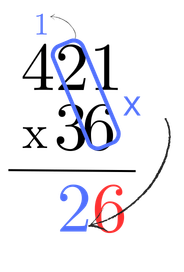
\includegraphics[width=0.25\linewidth]{imagens/mult_36_421_3.png}
        \label{fig:multi_36_421_3}
    \end{figure}

    \begin{figure}[H]
        \centering
        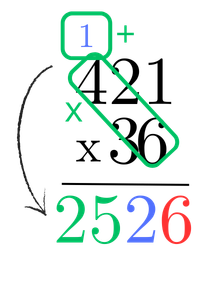
\includegraphics[width=0.25\linewidth]{imagens/mult_36_421_4.png}
        \label{fig:multi_36_421_4}
    \end{figure}

    E obtemos o primeiro resultado. Pulamos uma linha para baixo e deslocamos uma casa para esquerda para calcular o próximo resultado.

    \begin{figure}[H]
        \centering
        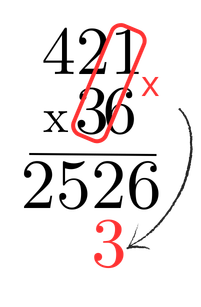
\includegraphics[width=0.25\linewidth]{imagens/mult_36_421_5.png}
        \label{fig:multi_36_421_5}
    \end{figure}

    \begin{figure}[H]
        \centering
        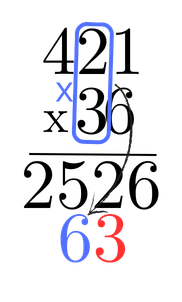
\includegraphics[width=0.24\linewidth]{imagens/mult_36_421_6.png}
        \label{fig:multi_36_421_6}
    \end{figure}

    \begin{figure}[H]
        \centering
        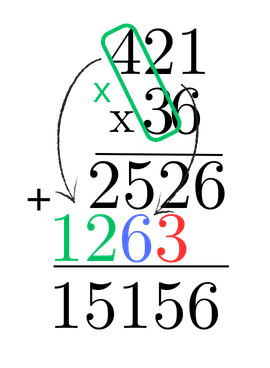
\includegraphics[width=0.33\linewidth]{imagens/mult_36_421_7.png}
        \label{fig:multi_36_421_7}
    \end{figure}

    E por fim somamos o primeiro resultado (\(2526\)) com o segundo resultado (\(1263\)), que é igual a \(15156\).
    
    \begin{figure}[H]
        \centering
        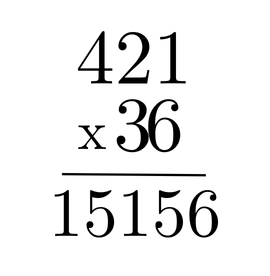
\includegraphics[width=0.3\linewidth]{imagens/mult_36_421_8.png}
        \label{fig:multi_36_421_8}
    \end{figure}
\end{exemplo}

O(a) aluno(a) arrependido(a) que antes menosprezava o procedimento agora pensa: ``E se.. eu.. adicionar mais um algarismo no número de baixo da multiplicação?''. Exatamente como esperado, adicionamos uma \textbf{terceira}/ou mais linhas abaixo das anteriores na parte dos resultados parciais, sempre deslocando uma casa para esquerda a cada linha que descemos.

\begin{exemplo}
    Considere a multiplicação de 942 por 2004. 

    \begin{figure}[H]
        \centering
        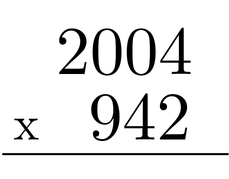
\includegraphics[width=0.2\linewidth]{imagens/mult_942_2004_1.png}
        \label{fig:mult_942_2004_1}
    \end{figure}

    Começamos o procedimento da mesma maneira, número menor abaixo do número maior, com casa das unidades se encontrando. Selecionamos o primeiro algarismo da esquerda do número de baixo (2) e multiplicamos por todos algarismos de cima, lembrando que fazemos isso da direita para esquerda.
    
    \begin{figure}[H]
        \centering
        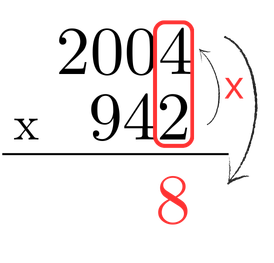
\includegraphics[width=0.2\linewidth]{imagens/mult_942_2004_2.png}
        \label{fig:mult_942_2004_2}
    \end{figure}

    \begin{figure}[H]
        \centering
        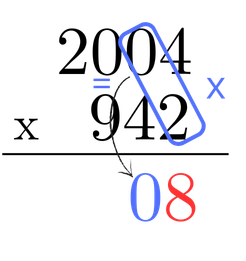
\includegraphics[width=0.2\linewidth]{imagens/mult_942_2004_3.png}
        \label{fig:mult_942_2004_3}
    \end{figure}

    \begin{figure}[H]
        \centering
        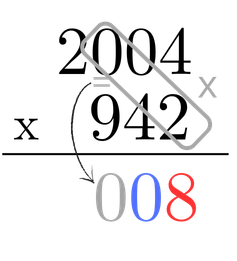
\includegraphics[width=0.2\linewidth]{imagens/mult_942_2004_4.png}
        \label{fig:mult_942_2004_4}
    \end{figure}

    \begin{figure}[H]
        \centering
        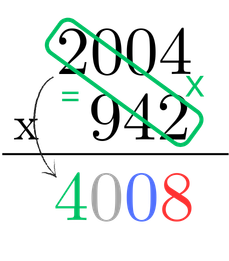
\includegraphics[width=0.2\linewidth]{imagens/mult_942_2004_5.png}
        \label{fig:mult_942_2004_5}
    \end{figure}

    Finalizados com o primeiro, passamos para o segundo algarismo (4) e multiplicamos por todos os de cima. Relembrando, o resultado agora colocamos uma linha abaixo do resultado anterior e com uma casa deslocada para esquerda. 
    
    \begin{figure}[H]
        \centering
        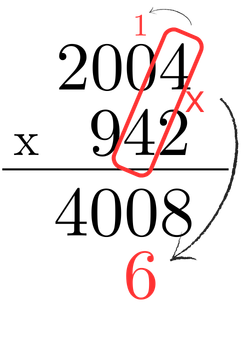
\includegraphics[width=0.2\linewidth]{imagens/mult_942_2004_6.png}
        \label{fig:mult_942_2004_6}
    \end{figure}

    \begin{figure}[H]
        \centering
        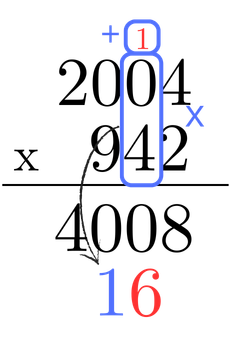
\includegraphics[width=0.2\linewidth]{imagens/mult_942_2004_7.png}
        \label{fig:mult_942_2004_7}
    \end{figure}

    \begin{figure}[H]
        \centering
        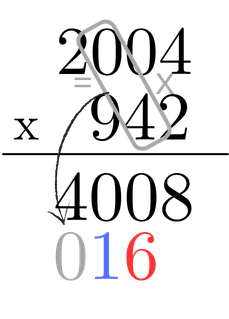
\includegraphics[width=0.2\linewidth]{imagens/mult_942_2004_8.png}
        \label{fig:mult_942_2004_8}
    \end{figure}

    \begin{figure}[H]
        \centering
        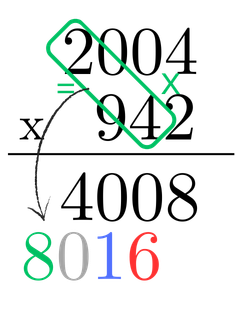
\includegraphics[width=0.2\linewidth]{imagens/mult_942_2004_9.png}
        \label{fig:mult_942_2004_9}
    \end{figure}

    E da mesma maneira que fizemos para os outros, para o terceiro algarismo não será diferente. Multiplicamos ele por todos de cima, com o resultado sendo adicionado abaixo do anterior e com uma casa deslocada para esquerda.
    
    \begin{figure}[H]
        \centering
        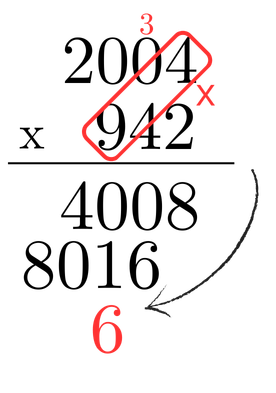
\includegraphics[width=0.24\linewidth]{imagens/mult_942_2004_10.png}
        \label{fig:mult_942_2004_10}
    \end{figure}

    \begin{figure}[H]
        \centering
        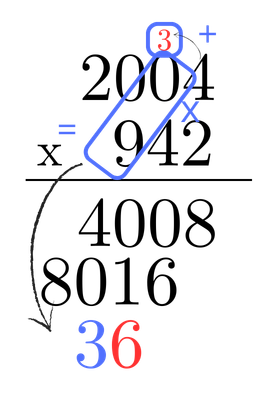
\includegraphics[width=0.24\linewidth]{imagens/mult_942_2004_11.png}
        \label{fig:mult_942_2004_11}
    \end{figure}

    \begin{figure}[H]
        \centering
        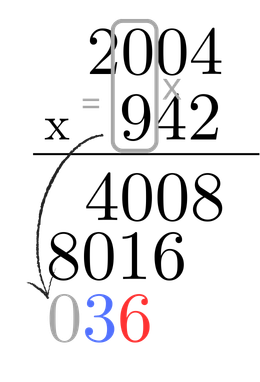
\includegraphics[width=0.24\linewidth]{imagens/mult_942_2004_12.png}
        \label{fig:mult_942_2004_12}
    \end{figure}

    \begin{figure}[H]
        \centering
        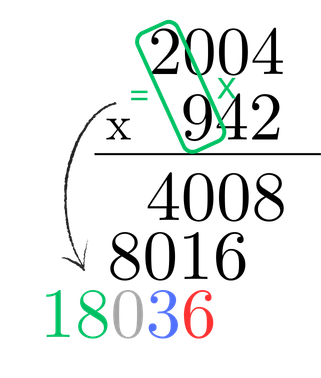
\includegraphics[width=0.27\linewidth]{imagens/mult_942_2004_13.png}
        \label{fig:mult_942_2004_13}
    \end{figure}

    E finalizados todos os algarismos do número de baixo, nós somamos todos os resultados parciais (respeitando as regras já vistas em adição) e encontramos nosso resultado final.
    
    \begin{figure}[H]
        \centering
        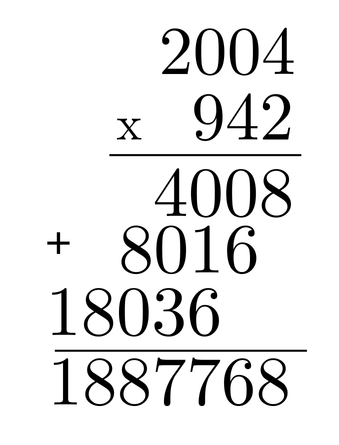
\includegraphics[width=0.27\linewidth]{imagens/mult_942_2004_14.png}
        \label{fig:mult_942_2004_14}
    \end{figure}
\end{exemplo}

Algo interessante para repararmos no último exemplo (e em boa parte dos outros também) é que a soma dos resultados parciais não é simplesmente \(4.008+8.016+18.036\) e sim \(4.008+80.160+1.803.600\). No entanto, esses ``zeros'' a mais na direita dos números não aparecem, exatamente porque fomos deslocando para esquerda a medida que descemos nas linhas, e então eles ``não são'' necessários. Mas tenha em mente que eles existem ali e que essa é a razão de deslocarmos para esquerda.

Outro fato interessante que o(a) estudante também já deve ter notado é: o \textit{trabalho exaustivo} de quem teve que fazer todas essas artes dos dispositivos práticos. Porém, todo conteúdo dessa apostila foi feito com amor e carinho para que você, estudante, possa se sentir o mais confortável possível em absorver as informações aqui passadas. Então, não deixe de reservar um momento da sua leitura para conferir e agradecer (mesmo que mentalmente) quem foram as(os) responsáveis por esse belo trabalho.


\newpage
\section{Divisão}

Como no caso da subtração, também podemos pensar na divisão de duas maneiras diferentes:

\begin{enumerate}
    \item Como a operação inversa da multiplicação, interpretada como um tipo de soma, mais especificamente uma soma de frações;
    \item Como uma multiplicação de um número por uma fração.
\end{enumerate}

Mas antes de iniciar essa discussão, vamos primeiramente revisar o conceito de fração, que aparece em ambas as “definições” acima.

\subsection{Frações}
\label{fracoes}
Fração é um número composto por duas partes: o \textbf{numerador} e o \textbf{denominador}. Para entender melhor o que eles representam, vamos imaginar uma pizza dividida em 8 pedaços:

\begin{figure}[H]
    \centering
    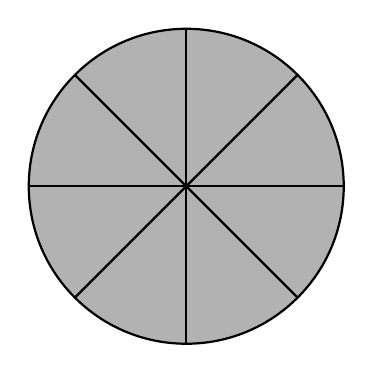
\begin{tikzpicture}
  \foreach \i in {0,45,...,315} {
    \fill[gray!60] (0,0) -- (\i:2) arc (\i:\i+45:2) -- cycle;
  }
  \draw[thick] (0,0) circle (2);
  \foreach \i in {0,45,...,315} {
    \draw[thick] (0,0) -- (\i:2);
  }
\end{tikzpicture}
\end{figure}

Agora, vamos pegar 2 fatias dessa pizza:

\begin{figure}[H]
    \centering
    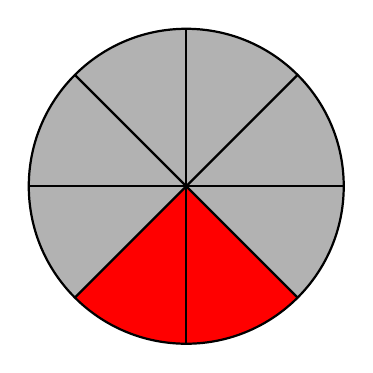
\begin{tikzpicture}

\def\R{2} % Raio da pizza

% Desenha as fatias
\foreach \i in {0,...,7} {
  \pgfmathsetmacro{\start}{\i*45}
  \pgfmathsetmacro{\end}{(\i+1)*45}
  % Cor vermelha para as duas últimas fatias (posição 5 e 6)
  \ifnum\i=5
    \fill[red] (0,0) -- (\start:\R) arc (\start:\end:\R) -- cycle;
  \else\ifnum\i=6
    \fill[red] (0,0) -- (\start:\R) arc (\start:\end:\R) -- cycle;
  \else
    \fill[gray!60] (0,0) -- (\start:\R) arc (\start:\end:\R) -- cycle;
  \fi\fi
}

% Contorno do círculo
\draw[thick] (0,0) circle (\R);

% Linhas divisórias
\foreach \a in {0,45,...,315} {
  \draw[thick] (0,0) -- (\a:\R);
}

\end{tikzpicture}
\end{figure}

Observe que pegamos 2 pedaços de um total de 8 pedaços. Então, nossa quantidade de fatias pode ser escrita na forma da seguinte fração:

\begin{equation}
    \frac{2}{8}
\end{equation}\\

E podemos ler essa fração como ``\textbf{dois oitavos}'' da pizza, que representa 2 partes de um total de 8.\\

\begin{exemplo}
    Sejam A = 3 e B = 5, se quisermos montar uma fração A/B temos:

    \begin{equation}
        \frac{A}{B} = \frac{3}{5}
    \end{equation}

    A fração acima tem como numerador 3 e como denominador 5, ou seja, estamos considerando 3 partes de um total de 5 partes. 
\end{exemplo}


\subsubsection{SOMA DE FRAÇÕES}

As frações também são números, elas só são \textit{diferentes}, e não merecem ser tratadas de outro jeito por isso. Em outra apostila, vamos conversar mais sobre Teoria dos Conjuntos e entender melhor o que são números Naturais (\(\mathbbm{N}\)), Inteiros (\(\mathbbm{Z}\)), Racionais (\(\mathbbm{Q}\)), Irracionais (\(\mathbbm{I}\)) e Reais (\(\mathbbm{R}\)). Quem sabe até o que são números Complexos (\(\mathbbm{C}\)).

Bom, frações são números que chamamos de racionais, o que isso significa não será importante para nós no momento. Dito isso, também podemos operar com elas: somar, subtrair, multiplicar, dividir, elevar à uma potência, tirar raiz etc. Mas como fazer isso exatamente? É o que veremos agora.

Como discutido anteriormente, sabemos que frações possuem tanto numerador quanto denominador. Para que possamos realizar a soma de duas ou mais frações, é importante que todas estejam com o \textbf{mesmo denominador}. Se elas tiverem denominadores diferentes, é como se estivéssemos tentando somar pedaços de pizza de tamanho diferentes, e não vários pedaços de mesmo tamanho.

Caso não tenha ficado subentendido, vamos ter certeza: quando os denominadores já forem iguais podemos simplesmente pular as etapas que vamos discutir, e somente somar sobre um denominador comum. Por exemplo:

\begin{exemplo}
    Considere a soma das seguintes frações:
    \begin{equation}
        \frac{2}{5}+\frac{7}{5}
    \end{equation}

    \begin{equation}
        =\frac{2+7}{5}
    \end{equation}

    \begin{equation}
        =\frac{9}{5}
    \end{equation}
\end{exemplo}

No entanto, sabemos que nem sempre vamos ter frações com o mesmo denominador, então nos resta aprender a como ``converter'' essas frações para que elas fiquem no denominador que quisermos. Uma maneira elegante de realizar isso é através do \textbf{Mínimo Múltiplo Comum} (MMC), que será discutido no Capítulo 4. Porém, no momento, utilizaremos uma maneira \textit{não elegante} de realizar esse procedimento, sem utilizar MMC. Vejamos.

\newpage
\begin{tcolorbox}[title = Procedimento para Soma de Frações]
    Vamos utilizar letras para representarem números quaisquer, pois dessa maneira podemos escrever um procedimento geral para soma e que funciona para qualquer número no lugar das letras.\\
    
    Quando quisermos realizar a soma de frações do tipo:

    \begin{equation}
        \frac{A_1}{B_1}+\frac{A_2}{B_2}+\frac{A_3}{B_3}+\cdots
    \end{equation}

    Temos que todos os numeradores são diferentes, assim como todos os denominadores. Um jeito \textit{porco} de criar um denominador comum é simplesmente \textbf{multiplicar todos denominadores}, veja:

    \begin{equation}
        \frac{???}{B_1 \times B_2 \times B_3}
    \end{equation}

    Ok, mas o que exatamente vai em cima dessa fração como numerador? Temos um procedimento para descobrir:
    
    \begin{enumerate}
        \item Pegar esse denominador monstruoso que criamos e dividir pelo respectivo denominador de cada fração;
        \item Pegamos o resultado dessa divisão e multiplicamos pelo respectivo numerador de cada fração;
        \item Pronto, mantemos o sinal de soma ou subtração original.
    \end{enumerate} 

    Ficando:

    \begin{equation}
        \frac{(B_2\times B_3)\times A_1+(B_1\times B_3)\times A_2 + (B_1\times B_1) \times A_3}{B_1\times B_2 \times B_3}
    \end{equation}
\end{tcolorbox}

Sim, nós criamos um monstro... visualmente horrível e aparentemente difícil de resolver. Mas com alguns exemplos será possível perceber que não é tão feio e difícil assim, e já é uma introdução de como será feito usando MMC. Vejamos:

\begin{exemplo} \label{ex_primeiro_soma_frac}
    Considere a soma das seguintes frações:

    \begin{equation}
        \frac{\textcolor{red}{1}}{\textcolor{red}{2}} + \frac{\textcolor{blue}{1}}{\textcolor{blue}{3}} + \frac{\textcolor{purple}{1}}{\textcolor{purple}{5}}
    \end{equation}

    Vamos seguir nosso procedimento. Primeiro multiplicar todos os denominadores:

    \begin{equation}
        \frac{???}{\textcolor{red}{2}\times\textcolor{blue}{3}\times\textcolor{purple}{5}}
    \end{equation}

    Agora, precisamos dividir esse novo denominador individualmente por cada denominador antigo:

    \begin{equation}
        \frac{\textcolor{red}{2}\times\textcolor{blue}{3}\times\textcolor{purple}{5}}{\textcolor{red}{2}} \quad \text{e} \quad \frac{\textcolor{red}{2}\times\textcolor{blue}{3}\times\textcolor{purple}{5}}{\textcolor{blue}{3}} \quad \text{e} \quad \frac{\textcolor{red}{2}\times\textcolor{blue}{3}\times\textcolor{purple}{5}}{\textcolor{purple}{5}}
    \end{equation}

    De cada divisão, podemos simplificar os números que forem iguais em cima e em baixo:

    \begin{equation}
        \frac{\cancel{2}\times3\times5}{\cancel{2}}=3\times5
    \end{equation}

    \begin{equation}
        \frac{2\times\cancel{3}\times5}{\cancel{3}}=2\times5 
    \end{equation}

    \begin{equation}
        \frac{2\times3\times \cancel{5}}{\cancel{5}}=2\times3 
    \end{equation}

    Esses valores que sobraram agora, vão ser multiplicados pelos numeradores das suas respectivas frações:

    \begin{equation}
        \frac{(3\times5)\times\textcolor{red}{1}+(2\times5)\times \textcolor{blue}{1} + (2\times3)\times \textcolor{purple}{1}}{2\times3\times5}
    \end{equation}

    Agora sim, temos a nossa fração ``convertida'' para um mesmo denominador, podemos somar os numeradores.

    \begin{equation}
        =\frac{(15)\times1+(10)\times1 + (6)\times1}{30}
    \end{equation}

    \begin{equation}
        =\frac{15+10+1}{30}
    \end{equation}

    \begin{equation}
        =\frac{26}{30}
    \end{equation}

    Então, podemos dizer que a soma das três frações iniciais é igual a esse resultado final:

    \begin{equation}
        \frac{1}{2}+\frac{1}{3}+\frac{1}{5}=\frac{26}{30}
    \end{equation}

    O interessante de reparar é que o denominador final da resposta não é igual a nenhum denominador anterior, e isso pode acontecer sem problema.
\end{exemplo}

\textcolor{red}{Observação}: A fração resultante do Exemplo \ref{ex_primeiro_soma_frac} ainda poderia ser \textbf{simplificada}, para encontrar uma \textbf{fração equivalente} com números menores. Isso será discutido em breve.

Vejamos outro exemplo.

\begin{exemplo}
    Considere a seguinte soma de frações:

    \begin{equation}
        \frac{2}{3}+\frac{5}{7}
    \end{equation}

    Seguindo nosso procedimento:

    \begin{equation}
        \frac{???}{3\times7}
    \end{equation}

    Dividindo o denominador resultante por cada denominador:
    
    \begin{equation}
        \frac{3\times7}{3}=\frac{\cancel{3}\times7}{\cancel{3}}=7
    \end{equation}

    \begin{equation}
        \frac{3\times7}{7}=\frac{3\times\cancel{7}}{\cancel{7}}=3
    \end{equation}

    Multiplicando pelo numerador de cada fração:

    \begin{equation}
        =\frac{(7)\times2+(3)\times5}{3\times7}
    \end{equation}

    Agora podemos resolver:

    \begin{equation}
        =\frac{14+15}{21}
    \end{equation}

    Então obtemos:
    
    \begin{equation}
        =\frac{29}{21}
    \end{equation}
\end{exemplo}

E quando tivermos a soma de uma fração por um número? Simples, só lembrarmos que todo número dividido por 1 é ele mesmo, então:

\begin{tcolorbox}[title=Soma de fração e número]
    Considere a seguinte soma:

    \begin{equation}
        A + \frac{A}{B}
    \end{equation}

    Lembrando que A e A/1 são a mesma coisa, então:

    \begin{equation}
        \frac{A}{1} + \frac{A}{B}
    \end{equation}

    E pronto, retornamos ao caso de soma de duas frações
\end{tcolorbox}

Um exemplo numérico para ajudar:

\begin{exemplo}
    Considere a seguinte soma:

    \begin{equation}
        2 + \frac{3}{5}
    \end{equation}

    Como vimos anteriormente, 2 e 2/1 são a mesma coisa, então:

    \begin{equation}
        \frac{2}{1} + \frac{3}{5}
    \end{equation}

    Encontrando um denominador comum:

    \begin{equation}
        \frac{???}{1\times5}
    \end{equation}

    Dividindo pelos denominadores originais:

    \begin{equation}
        \frac{1\times5}{1}=5
    \end{equation}

    \begin{equation}
        \frac{1\times 5}{5}=1
    \end{equation}

    Agora multiplicando esses resultados pelos numeradores:

    \begin{equation}
        =\frac{(5)\times2 + (1)\times 3}{1\times5}
    \end{equation}

    \begin{equation}
        =\frac{10+3}{5}
    \end{equation}
    \begin{equation}
        =\frac{13}{5}
    \end{equation}

    Logo, temos que a \textbf{soma de 2 com 3/5 é igual a 13/5}.
\end{exemplo}


\subsubsection{SUBTRAÇÃO DE FRAÇÕES}

Para subtrações de frações, o procedimento se mantém igual ao de soma, só que agora vamos colocar o sinal de (-) ao invés de (+), o que não é uma novidade e seria tedioso de se repetir. Para deixar mais interessante, vamos misturar somas \textbf{e} subtrações de frações.

\begin{exemplo}
    Considere a soma e subtração das seguintes frações:

    \begin{equation}
        \frac{11}{13}+\frac{1}{7}-\frac{9}{21}
    \end{equation}

    Calculando o denominador comum:

    \begin{equation}
        \frac{???}{13\times7\times21}
    \end{equation}

    Dividindo por cada denominador das frações:

    \begin{equation}
        \frac{13\times7\times21}{13}=\frac{\cancel{13}\times7\times21}{\cancel{13}} = 7\times21
    \end{equation}
    
    \begin{equation}
        \frac{13\times7\times21}{7} = \frac{13\times\cancel{7}\times21}{\cancel{7}} = 13\times21
    \end{equation}
    
    \begin{equation}
        \frac{13\times7\times21}{21} = \frac{13\times7\times\cancel{21}}{\cancel{21}} = 13\times 7
    \end{equation}

    Multiplicando cada resultado pelo numerador da sua respectiva fração:

    \begin{equation}
        \frac{(7\times21)\times11\textcolor{red}{+}(13\times21)\times1\textcolor{red}{-}(13\times 7)\times9}{13\times7\times21}
    \end{equation}

    Perceba que a diferença é que ``aparece'' um sinal de menos no terceiro numerador, pois era a fração que estava subtraindo, nada demais. E agora podemos fazer essa conta horrorosa.

    \begin{equation}
        =\frac{(147)\times11+(273)\times1-(91)\times9}{1911}
    \end{equation}
    
    \begin{equation}
        =\frac{1617+273-819}{1911}
    \end{equation}

    Por fim:
    
    \begin{equation}
        =\frac{1071}{1911}
    \end{equation}
\end{exemplo}

Ou seja, nem sempre a vida é bela com números bonitos. Essa é a realidade. Esse exemplo não ficaria muito menos feio usando MMC, então estejam preparados para realizarem contas esquisitas em muitas listas de exercícios e provas pela frente.

Poderíamos ficar o restante da apostila resolvendo somas e subtrações de frações. Porém, com o procedimento descrito junto com os exemplos que vimos, você já é capaz de resolver qualquer outro problema relacionado. Agora o trabalho está em suas mãos, de resolver uma quantidade exaustiva de exercícios para fixar o conteúdo.

\subsubsection{MULTIPLICAÇÃO DE FRAÇÕES}

Para nós, meros estudantes da matemática, essa seção de Multiplicação de Frações será o equivalente a um oásis no deserto. Aproveite para recuperar o fôlego e tomar uma água.

Multiplicar duas ou mais frações é mais direto do que parece, a \textbf{única ``regra'}' é que devemos multiplicar somente os numeradores entre si, assim como os denominadores entre si, não podendo misturar multiplicações da parte de cima com a de baixo. Simples! Vejamos alguns exemplos.

\begin{exemplo}
    Considere a multiplicação das seguintes frações:

    \begin{equation}
        \frac{2}{3}\times\frac{5}{7}
    \end{equation}

    Simplesmente multiplicamos os números dos numeradores, e os números dos denominadores (lembrando de não misturar):

    \begin{equation}
        =\frac{2\times5}{3\times7}
    \end{equation}

    \begin{equation}
        =\frac{10}{21}
    \end{equation}

    Pronto, fim! Não precisamos nos preocupar com denominador comum nem nada do tipo.
\end{exemplo}

Podemos também multiplicar frações com sinais diferentes, sem muita complicação.

\begin{exemplo}
    Considere a multiplicação das seguintes frações:

    \begin{equation}
        \left(-\frac{2}{4}\right)\times\frac{7}{5}
    \end{equation}

    Da nossa regrinha de sinais, sabemos que (-)\(\times\)(+) = (-), então:

    \begin{equation}
        =-\frac{2\times7}{4\times5}
    \end{equation}

    \begin{equation}
        =-\frac{14}{20}
    \end{equation}
\end{exemplo}


\subsubsection{DIVISÃO DE FRAÇÕES}
Quase tão simples quanto multiplicar duas frações, a divisão de frações será um processo de \textbf{transformar o problema em uma multiplicação de frações}, pois a partir daí nós já sabemos resolver com muita \textit{maestria}.

Quando temos duas frações dividindo, podemos visualizar o problema como uma \textbf{fração de frações}, onde a fração de cima seria o numerador e a fração de baixo seria o denominador. Sem tentar complicar muito, o procedimento é simples:

\begin{tcolorbox}[title = Procedimento para Divisão de Frações]

    \begin{enumerate}
        \item Manter a fração de cima fixa, inalterada;
        \item Inverter a fração de baixo, trocando o seu numerador pelo denominador e vice-versa.
        \item Multiplicar as duas frações que resultaram desse processo.
    \end{enumerate}
\end{tcolorbox}

Vejamos alguns exemplos.

\begin{exemplo}
    Considere a divisão das seguintes frações:

    \begin{equation}
        \frac{2}{3} \quad e \quad \frac{5}{7}
    \end{equation}
    
    Por uma questão de espaço, vamos chamar essas duas frações de 2/3 e 5/7, então temos:
    
    \begin{equation}
        \frac{2/3}{\textcolor{red}{5}/\textcolor{blue}{7}}
    \end{equation}

    De acordo com nosso procedimento, temos que manter a primeira e inverter a segunda, e então multiplicar as duas, então:

    \begin{equation}
        =\frac{2}{3}\times\frac{\textcolor{blue}{7}}{\textcolor{red}{5}}
    \end{equation}

    Daí chegamos em uma situação que já sabemos resolver.

    \begin{equation}
        =\frac{2\times7}{3\times5}
    \end{equation}

    \begin{equation}
        =\frac{14}{15}
    \end{equation}

    Então, podemos dizer que a \textbf{divisão de 2/3 por 5/7 é igual a 14/15}.
\end{exemplo}

Uma dúvida que pode surgir é quando temos a divisão de um número por uma fração \textbf{ou} uma fração por um número. Vamos ver exemplos dos dois casos.

\begin{exemplo}
    Considere a divisão de uma fração por um número:

    \begin{equation}
        \frac{2/3}{5}
    \end{equation}

    Apesar de parecer difícil, fica muito mais simples quando lembramos que todo número (N) pode ser escrito como uma fração N/1... pois todo número dividido por 1 é ele mesmo!

    Vamos reescrever esse problema, substituindo o 5 por 5/1:

    \begin{equation}
        \frac{2/3}{5/1}
    \end{equation}

    E pronto, voltamos para o cenário de divisão de frações. Então nós mantemos a fração de cima, invertemos a de baixo e multiplicamos os resultados:

    \begin{equation}
        =\frac{2}{3}\times\frac{1}{5}
    \end{equation}

    \begin{equation}
        =\frac{2\times1}{3\times5}
    \end{equation}

    \begin{equation}
        =\frac{2}{15}
    \end{equation}

    Então, podemos dizer que \textbf{2/3 dividido por 5 é igual a 2/15}.
    
\end{exemplo}

O outro cenário que comentamos é um número dividido por uma fração. Mas você verá que o procedimento também é o mesmo.

\begin{exemplo}
    Considere a divisão de um número por uma fração:

    \begin{equation}
        \frac{10}{5/7}
    \end{equation}

    Novamente, vamos visualizar o número 10 como uma fração de 10/1. 

    \begin{equation}
        =\frac{10/1}{5/7}
    \end{equation}

    E novamente caímos no caso de divisão de frações. Resolvendo:

    \begin{equation}
        =\frac{10}{1}\times\frac{7}{5}
    \end{equation}

    \begin{equation}
        =\frac{10\times7}{1\times5}
    \end{equation}

    \begin{equation}
        =\frac{70}{5}
    \end{equation}
\end{exemplo}

Como dito anteriormente, muitos dos resultados que encontramos ainda poderiam ser simplificados, para frações com números menores. Ou seja, frações que possuem o mesmo \textbf{valor} mas são escritas de \textbf{maneira diferente}. Chamamos esses casos de frações equivalentes.

\subsubsection{FRAÇÕES EQUIVALENTES}

Então, queremos escrever a mesma fração de várias maneiras diferentes, seja para ajudar a resolver algum problema, ou mesmo para aprender a simplificar frações.

Acredite ou não, o grande \textit{segredo} de frações equivalentes é saber utilizar o ``elemento neutro'' da multiplicação. Em todos os casos o que estamos fazendo na prática é multiplicando por 1. Mas por que isso? Exatamente pela razão de não querermos \textbf{alterar o resultado}, somente queremos reescrever com ``outras palavras'' (outros números no caso, mas a ideia é a mesma).

A ideia de maneira geral é a seguinte:

\begin{exemplo}
    Se tivermos uma fração do tipo:

    \begin{equation}
        \frac{A}{B}
    \end{equation}

    E queremos reescrever ela sem mudar o resultado. Primeiro, vamos concordar que um número \textbf{N} divido por ele mesmo é igual a 1:

    \begin{equation}
        \frac{N}{N}=1
    \end{equation}

    Sabemos que multiplicar por 1 não altera o resultado (elemento neutro), então:

    \begin{equation}
        \frac{A}{B}\times \frac{N}{N} =\frac{A}{B} \times 1 = \frac{A}{B}
    \end{equation}

    Mas ao invés de dividir N, multiplicar por N e igualar a 1, vamos deixar a fração intacta e realizar a multiplicação de frações:

    \begin{equation}
        \frac{A}{B}\times \frac{N}{N} = \frac{A\times N}{B \times B} = \frac{AN}{BN}
    \end{equation}

    Em uma primeira impressão, parece que a fração AN/BN é diferente de A/B, \textbf{mas} sabemos que não é o caso, na verdade elas são \textbf{equivalentes}... pois na prática apenas multiplicamos por 1.
\end{exemplo}

Vamos ver alguns exemplos numéricos para esclarecer o problema.

\begin{exemplo}
    Considere a seguinte fração:

    \begin{equation}
        \frac{1}{2}
    \end{equation}

    Podemos reescrever ela de infinitas maneiras seguindo o nosso procedimento. Por exemplo, vamos multiplicá-la por 3/3:

    \begin{equation}
        \frac{1}{2}\times\frac{3}{3}=\frac{3\times1}{2\times3}=\frac{3}{6}
    \end{equation}

    Logo, sabemos que 3/6 e 1/2 são frações equivalentes, pois na prática só realizamos a multiplicação por 1 (3/3). 
\end{exemplo}

A princípio pode parecer uma coisa boba, mas que na verdade vai nos ajudar muito. Por exemplo, se quiséssemos encontrar um denominador comum mais rápido:

\begin{exemplo}
    Considere a seguinte soma:

    \begin{equation}
        =3+\frac{5}{7}
    \end{equation}

    Já sabemos que 3 pode ser reescrito como 3/1. Com isso, se multiplicarmos 3/1 por 7/7, teríamos: 

    \begin{equation}
        =\frac{3}{1}\times\frac{7}{7} + \frac{5}{7}
    \end{equation}

    \begin{equation}
        =\frac{3\times7}{1\times7}+ \frac{5}{7}
    \end{equation}

    \begin{equation}
        =\frac{21}{7}+ \frac{5}{7}
    \end{equation}

    E \textit{voilà}, temos um denominador comum sem precisar fazer aquele procedimento que vimos na soma de frações. Então temos:

    \begin{equation}
        =\frac{26}{7}
    \end{equation}

    
\end{exemplo}

\subsection{Propriedades da Divisão}

Por fim, mas \textbf{mais importante}, temos que definir algumas propriedades essenciais para a operação de divisão.

\begin{enumerate}
    \item Divisão \textbf{não} é \textbf{comutativa}: \(A\div B\neq B\div A\) (exceto quando \(A=B\));
    \item Divisão \textbf{não} é \textbf{associativa}: \((A\div B)\div C \neq A\div(B\div C)\);
    \item Divisão por zero \textbf{não} é definida;
    \item Dividir zero por qualquer coisa (exceto zero) é sempre zero;
    \item Dividir um número (N) por 1 é sempre o próprio número: \(N\div1=N\).
    
\end{enumerate}

\subsection{Dispositivo Prático}

Revisado o conceito de fração, vamos conversar sobre divisão. A primeira maneira de se analisar a divisão nos diz que podemos considerá-la como uma soma de frações. Entenda da seguinte maneira: quando dividimos uma pizza em 8 pedaços (então, uma divisão por 8), estamos criando 8 fatias de tamanho 1/8 do total, de forma que, quando somamos todas as fatias temos:

\begin{equation}
    \frac{1}{8}+\frac{1}{8}+\frac{1}{8}+\frac{1}{8}+\frac{1}{8}+\frac{1}{8}+\frac{1}{8}+\frac{1}{8}=\frac{8}{8}=1
\end{equation}\\

E entenda esse valor de ``1'' como 100\%, ou seja, o total da pizza.\\
Por mais estranho que isso possa parecer, não se assuste, pois até agora estamos somente tentando entender o significado de uma divisão. Porém, o que queremos de fato é como efetuar o processo de divisão e obter um resultado. Vejamos alguns termos importantes antes:

\begin{figure}[H]
    \centering
    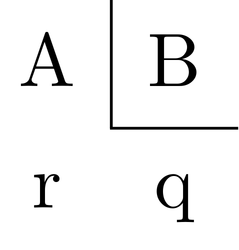
\includegraphics[width=0.25\linewidth]{imagens/divisao_esquema.png}
    \label{fig:divisao_esquema}
\end{figure}

Os termos \textbf{A} (\textbf{dividendo}) e \textbf{B} (\textbf{divisor}) são um pouco mais intuitivos e deixaremos para visualizarmos melhor em um exemplo numérico logo a frente.\\

Já o ``\textbf{q}'' (\textbf{quociente}) podemos entender como o número que precisamos multiplicar por B para encontrar o valor de A.\\

Imagine o ``\textbf{r}'' (\textbf{resto}) literalmente como o resto da divisão, ou seja, o que sobrou e “não podemos” dividir por B. Perceba que quando nossa divisão for exata, ou seja, A for \textbf{um múltiplo} de B, o resto será igual a zero.\\

Vejamos alguns exemplos numéricos:

\begin{exemplo}
    Considere a divisão de 30 por 5:

    \begin{figure}[H]
        \centering
        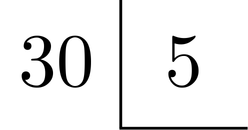
\includegraphics[width=0.25\linewidth]  {imagens/div_30_5_1.png}
        \label{fig:div_30_5_1}
    \end{figure}

    Montado nosso esquema de divisão, primeiro temos que identificar qual o primeiro algarismo ``contido'' dentro de 30 - unidade ou dezena - que será divisível por 5. Veja:\\

    \begin{enumerate}
        \item Começamos sempre a verificar os algarismos da esquerda pra direita:

        \begin{figure}[H]
            \centering
            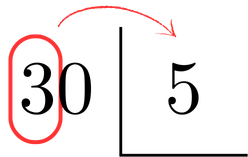
\includegraphics[width=0.25\linewidth]  {imagens/div_30_5_2.png}
            \label{fig:div_30_5_2}
        \end{figure}
        
        Da esquerda para a direita temos primeiro o algarismo ``3''. Considerando apenas ele a princípio, percebemos que não é suficiente fazer a divisão, pois ``3'' é menor do que ``5''. Então, passamos para o algarismo ao lado, ``0''. Sendo assim, devemos considerar o número como um todo, ``30'', porque ele sim será maior do que ``5''.

        \begin{figure}[H]
            \centering
            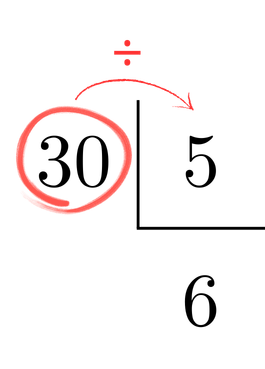
\includegraphics[width=0.25\linewidth]  {imagens/div_30_5_3.png}
            \label{fig:div_30_5_3}
        \end{figure}

        \item Sabemos pela tabuada que \(6\times5 = 30\), então o nosso quociente será o número 6 - que multiplicado por 5 nos dá o 30 que queremos.

        \begin{figure}[H]
            \centering
            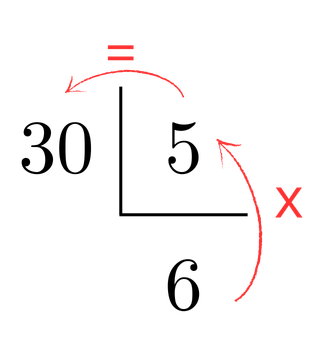
\includegraphics[width=0.3\linewidth]  {imagens/div_30_5_4.png}
            \label{fig:div_30_5_4}
        \end{figure}

        \item Escrevemos o resultado da multiplicação de 6 por 5 logo abaixo do nosso 30 (dividendo).

        \begin{figure}[H]
            \centering
            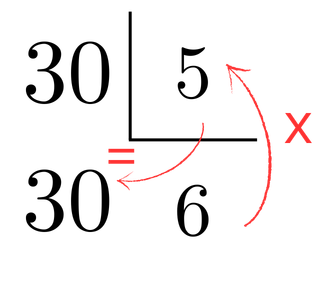
\includegraphics[width=0.27\linewidth]  {imagens/div_30_5_5.png}
            \label{fig:div_30_5_5}
        \end{figure}

        \item Efetuamos agora a subtração do 30 (dividendo) com o 30 (resultado da nossa multiplicação), encontrando, portanto, um resto igual a zero.

        \begin{figure}[H]
            \centering
            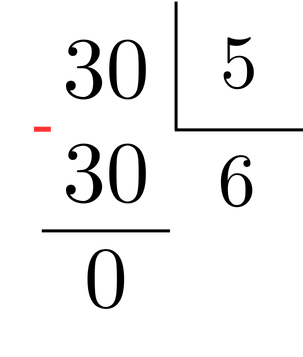
\includegraphics[width=0.25\linewidth]  {imagens/div_30_5_6.png}
            \label{fig:div_30_5_6}
        \end{figure}

        \item Quando chegamos em resto igual a zero, encerramos nossa divisão - nem sempre será o caso, veremos em outro exemplo. Vamos analisar os resultados.
    \end{enumerate}
    
    \begin{itemize}
        \item A = dividendo = 30
        \item B = divisor = 5
        \item q = quociente = 6
        \item r = resto = 0
    \end{itemize}

    Então, temos que \textbf{a divisão de 30 por 5 é igual a 6}.
\end{exemplo}

A princípio esse método não parece ser muito útil, mas isso deve-se aos valores escolhidos. E a partir de agora, ao invés de circularmos de vermelho o número vamos simplesmente usar aspas simples (') como separador. Vejamos um exemplo um pouco mais relevante.

\begin{exemplo}
    Considere a divisão de 128 por 2:

    \begin{figure}[H]
        \centering
        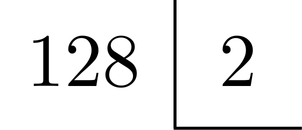
\includegraphics[width=0.25\linewidth] {imagens/div_128_2_1.png}
        \label{fig:div_128_2_1}
    \end{figure}

    Seguiremos os mesmos passos do exemplo anterior. Pegamos o primeiro algarismo da esquerda de 128, sempre:

    \begin{figure}[H]
        \centering
        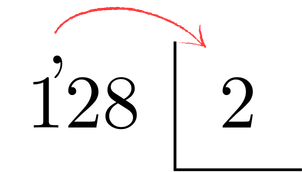
\includegraphics[width=0.25\linewidth] {imagens/div_128_2_2.png}
        \label{fig:div_128_2_2}
    \end{figure}

    Esse algarismo é igual a 1, sabemos que ele é menor do que nosso divisor 2, então continuamos para o próximo algarismo. 

    \begin{figure}[H]
        \centering
        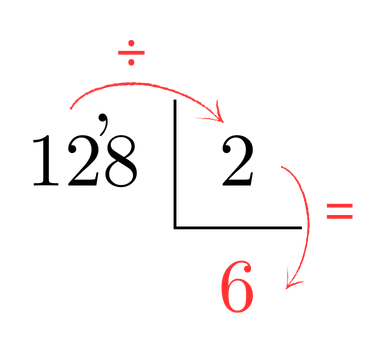
\includegraphics[width=0.3\linewidth] {imagens/div_128_2_3.png}
        \label{fig:div_128_2_3}
    \end{figure}

    Agora temos o número 12, que é maior do que nosso divisor, e podemos começar nosso processo. Temos que o resultado de \(6\times2 = 12\), então nosso primeiro algarismo do quociente será 6.

    \begin{figure}[H]
        \centering
        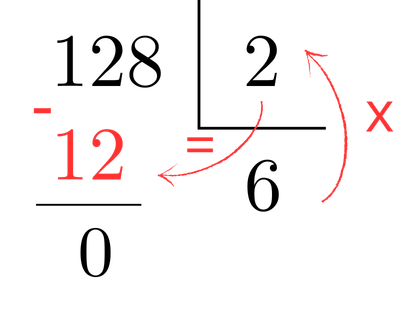
\includegraphics[width=0.3\linewidth] {imagens/div_128_2_4.png}
        \label{fig:div_128_2_4}
    \end{figure}

    Escrevemos então o resultado da primeira multiplicação abaixo do nosso número selecionado e efetuamos a subtração, obtendo o resultado zero. Porém, esse ainda não é nosso valor de resto, pois temos o número 8 lá em cima esperando. Eis o que faremos agora.

    \begin{figure}[H]
        \centering
        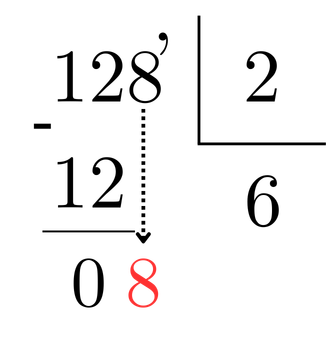
\includegraphics[width=0.25\linewidth] {imagens/div_128_2_5.png}
        \label{fig:div_128_2_5}
    \end{figure}

    ``Descemos'' o número 8 para que ele seja utilizado como nosso novo “número selecionado”. Temos que 8 é maior do que 2, então podemos continuar nossa divisão.

    \begin{figure}[H]
        \centering
        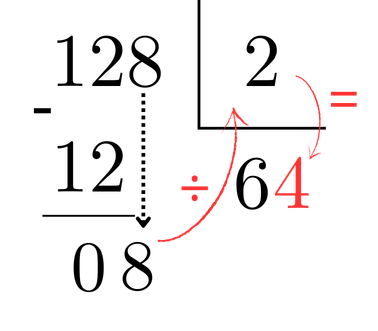
\includegraphics[width=0.3\linewidth] {imagens/div_128_2_6.png}
        \label{fig:div_128_2_6}
    \end{figure}

    Então, sabemos que \(4\times2 = 8\), que é o número que procuramos. Portanto, 4 é nosso próximo algarismo do quociente.

    \vspace{0.5cm}
        
    \textcolor{red}{Observação}: perceba que o algarismo zero foi selecionado juntamente com o 8, mas sabemos que 08 é o mesmo que somente 8, então não afetará nosso resultado. 

    \vspace{0.5cm}

    Continuamos então com o procedimento que já aprendemos, colocando o 8 (resultado de 4\(\times2\)) logo abaixo do nosso número selecionado. Efetuamos a subtração e encontramos o resultado zero. 

    \begin{figure}[H]
        \centering
        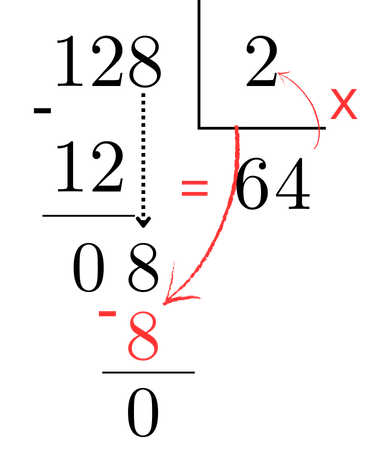
\includegraphics[width=0.3\linewidth] {imagens/div_128_2_7.png}
        \label{fig:div_128_2_7}
    \end{figure}

    Agora sim, chegamos ao fim da nossa divisão. Isso pois o resto é “zero” e não sobrou nenhum outro número para continuar o processo. Dessa forma, temos o seguinte:

    \begin{itemize}
        \item A = dividendo = 128
        \item B = divisor = 2
        \item q = quociente = 64
        \item r = resto = 0
    \end{itemize}
    Então, temos que o resultado de \textbf{128 dividido por 2 é igual a 64}.
\end{exemplo}

Caso tivéssemos outro algarismo após o 8, continuaríamos nosso procedimento da mesma maneira. Isso vai acontecer quando tivermos números grandes.

Com a esperança de que estamos ficando mais entendidos no assunto de divisão, vamos pegar alguns exemplos \textit{mais interessantes}.

\begin{exemplo}
    Considere agora a divisão de 17 por 3:

    \begin{figure}[H]
        \centering
        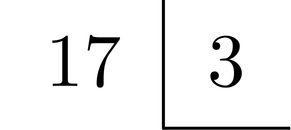
\includegraphics[width=0.25\linewidth] {imagens/div_17_3_1.png}
        \label{fig:div_17_3_1}
    \end{figure}

    Faremos o desenvolvimento completo, mas sem a presença de alguns dos textos auxiliares.

    \begin{figure}[H]
        \centering
        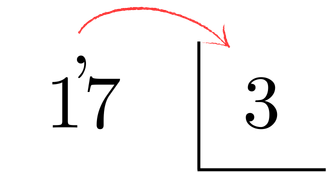
\includegraphics[width=0.25\linewidth] {imagens/div_17_3_2.png}
        \label{fig:div_17_3_2}
    \end{figure}

    Como 1 é menor do que 3, vamos prosseguir.

    \begin{figure}[H]
        \centering
        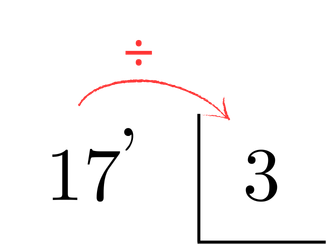
\includegraphics[width=0.25\linewidth] {imagens/div_17_3_3.png}
        \label{fig:div_17_3_3}
    \end{figure}

    Agora temos 17, um número maior que 3. Mas também perceba que temos um caso interessante e diferente. Não conhecemos, até o momento (pela tabuada), nenhum número que multiplicado por 3 que nos dá 17.

    \vspace{0.5cm}

    Em casos assim, o que tentaremos fazer é encontrar um número que multiplicado por 3 (divisor) nos dê um resultado \textbf{mais próximo} e \textbf{menor} do valor que estamos procurando. Veja:

    \begin{figure}[H]
        \centering
        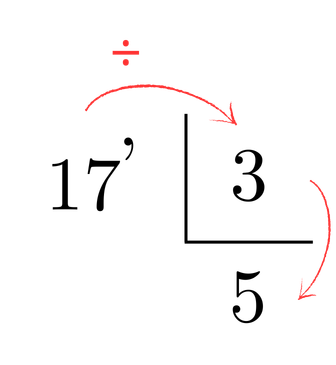
\includegraphics[width=0.25\linewidth] {imagens/div_17_3_4.png}
        \label{fig:div_17_3_4}
    \end{figure}

    Escolhemos o número 5 pelo fato de \(5\times3 = 15\) nos dar um valor próximo ao que procuramos, 17. Apesar do número 6 nos dar uma aproximação melhor (\(6\times3 = 18\)), não podemos usá-lo, pois o valor 18 é maior que 17 e pela nossa condição o resultado deve ser menor.

    \vspace{0.5cm}

    Definido isso, podemos continuar as operações como estávamos fazendo anteriormente. Efetuando a subtração, e assim por diante.

    \begin{figure}[H]
        \centering
        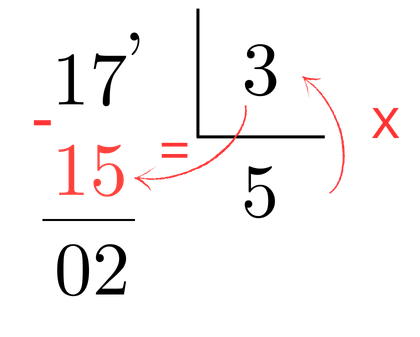
\includegraphics[width=0.3\linewidth] {imagens/div_17_3_5.png}
        \label{fig:div_17_3_5}
    \end{figure}

    Assumindo que o capítulo de subtração já está dominado, temos que o resultado de 17 - 15 = 2. Então, teríamos que continuar nosso procedimento até que o valor final - resto - fosse zero. No entanto, também temos que o resto 2 é menor do que 3 (divisor), não permitindo, então, que continuemos nossa divisão (por enquanto, veremos nos próximos capítulos).

    \vspace{0.5cm}

    Dessa forma, temos o seguinte resultado:

    \begin{itemize}
        \item A = dividendo = 17
        \item B = divisor = 3
        \item q = quociente = 5
        \item r = resto = 2
    \end{itemize}

    Temos que o resultado de \textbf{17 dividido por 3 é igual a 5 com resto 2} (por enquanto).
\end{exemplo}

\begin{tcolorbox}[title = Extra]
    No exemplo anterior, poderíamos pensar no resultado dessa divisão como: \(17 = 3\times5 + 2\) e extrapolar para uma regra geral que é:

    \begin{equation}
        A = q\times B + r
    \end{equation}

    Ou seja, o \textbf{dividendo} (A) é igual ao \textbf{divisor} (B) multiplicado pelo \textbf{quociente} (q) mais o \textbf{resto} (r).\\

    No entanto, veremos isso e suas aplicações com mais calma em outra oportunidade.
\end{tcolorbox}

\begin{exemplo}
    Considere a divisão de 4500 por 125. Como o nosso divisor tem 3 algarismos, já vamos começar a considerar o separador no primeiro 0 depois do 5, ficando com 450.

    \begin{figure}[H]
        \centering
        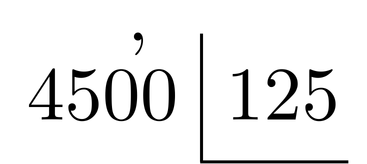
\includegraphics[width=0.3\linewidth] {imagens/div_4500_125_1.png}
        \label{fig:div_4500_125_1}
    \end{figure}

    Como 450 é maior do que 125, podemos realizar a divisão. Por \textit{azar}, não há número inteiro que multiplicado por 125 nos dê 450, então o mais próximo que conseguimos chegar (sendo menor) é multiplicando 3, que nos dá:

    \begin{figure}[H]
        \centering
        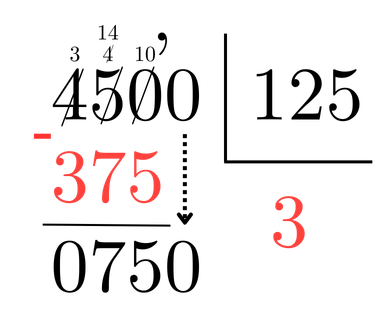
\includegraphics[width=0.3\linewidth] {imagens/div_4500_125_2.png}
        \label{fig:div_4500_125_2}
    \end{figure}

    E aqui não há nada de novo, multiplicamos, colocamos o resultado abaixo do número selecionado e realizamos a subtração. Sobrando um resto de 75, ``descemos'' o próximo algarismo 0 para continuar a nossa divisão.

    \begin{figure}[H]
        \centering
        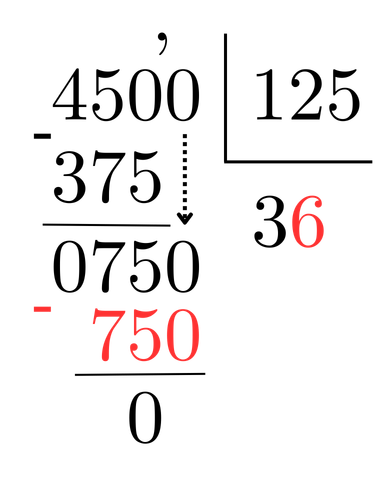
\includegraphics[width=0.3\linewidth] {imagens/div_4500_125_3.png}
        \label{fig:div_4500_125_3}
    \end{figure}

    E por fim temos o resultado final com resto zero.
\end{exemplo}

Vejamos um último exemplo.

\begin{exemplo}
    Considere a divisão de 78 por 124. A principio pode parecer estranho, pois o dividendo tem somente 2 algarismos e o divisor tem 3. Então, não há maneira de selecionar algarismos no dividendo para conseguir realizar a divisão, e agora?

    \begin{figure}[H]
        \centering
        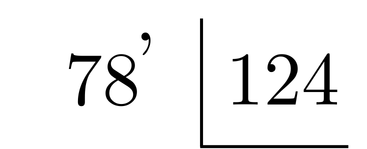
\includegraphics[width=0.3\linewidth] {imagens/div_78_124_1.png}
        \label{fig:div_78_124_1}
    \end{figure}

    Bom, pelo o que vimos até agora não podemos fazer nada. A título de visualização, o menor número que poderia ser multiplicado por 124 para que o resultado seja próximo de 78 mas menor, seria o número 0.

    \begin{figure}[H]
        \centering
        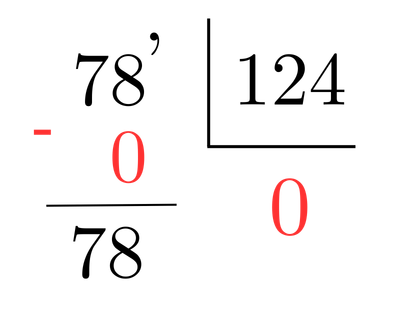
\includegraphics[width=0.3\linewidth] {imagens/div_78_124_2.png}
        \label{fig:div_78_124_2}
    \end{figure}

    Que nesse caso daria um resto também de 78, ou seja, inútil. Mas é o que daria para ser feito com nosso conhecimento até o momento.
\end{exemplo}

Esse exemplo nos dá a oportunidade perfeita de começarmos nossa conversa a respeito de uma nova família de números, que será o tema do nosso próximo capítulo: os números \textbf{decimais}.

\newpage
\section{Números Decimais}

Os números decimais por si só pertencem à um universo em particular, merecedores de sua própria apostila, mas aqui vamos tentar raspar a superfície de algumas maravilhas desse mundo. 

A princípio, podemos imaginar que os números decimais aparecem quando ``não conseguimos'' realizar a divisão totalmente, ou seja, quando a divisão tem resto diferente de zero. Em outra oportunidade vamos ver que defini-los dessa maneira não é o mais adequado, porque podemos ter resto zero em divisões com decimais também, mas em uma primeira abordagem acredito que vai ser o suficiente pra entender a ideia inicial. 

A grosso modo, números decimais são aqueles que precisamos de uma vírgula para escrevê-los. Os algarismos que tivermos antes da vírgula vamos chamar de \textbf{parte inteira}, os depois da vírgula vamos chamar de \textbf{parte decimal} e ela vai nos dizer quantas \textbf{casas decimais} ele possui. Assim como vimos no capítulo \ref{oque_sao_algarismos}, também vão existir divisões para o lado direito da primeira ordem (Unidades) dentro da Primeira Classe, que são chamadas de décimos, centésimos, milésimos e assim em diante.

Vejamos por exemplo o número 5,6789:

\begin{itemize}
    \item O algarismo 5, anterior a vírgula, chamamos de \textbf{parte inteira} do número decimal;
    \item O algarismo 6, logo após a virgula, chamamos de \textbf{décimo} do número decimal;
    \item O algarismo 7, na segunda casa após a vírgula, chamamos de \textbf{centésimo};
    \item O algarismo 8, na terceira casa após a vírgula, chamamos de \textbf{milésimo};
    \item O algarismo 9, na quarta casa após a vírgula, chamamos de \textbf{décimo de milésimo};
\end{itemize}

Antes de vermos como continuar nosso dispositivo prático de divisão, agora incluindo números decimais, vamos contemplar rapidamente a existência de 3 tipos deles: 1. \textbf{finitos}, 2. \textbf{infinitos periódicos} e 3. \textbf{infinitos não periódicos}. Além disso, também aprender como realizar as operações de soma, subtração e multiplicação utilizando esses novos números.

\subsection{Arredondamento de números}

\begin{tcolorbox}[title=IMPORTANTE]
    Até o momento não houve nenhuma conversa sobre \textbf{``arredondamento'' de números}. A grosso modo, sempre que tivermos o ``último'' algarismo desejado da parte decimal maior ou igual a 5, adicionamos/somamos 1 no algarismo anterior. Caso seja menor do que 5, deixamos o algarismo anterior sem alteração.
\end{tcolorbox}

Vamos fazer um pequeno parenteses aqui para apresentar alguns arredondamentos, esperando que o(a) aluno(a) consiga entender melhor.

Para arredondar um número, de forma geral, vai depender de quantas casas decimais nós queremos/precisamos depois da vírgula. Por exemplo, vamos trabalhar com o número 1,853728.

Esse número possuí um algarismo na parte inteira (1) e seis algarismos na parte decimal (853728). Porém, imagine que na verdade eu precisasse que ele tivesse somente 5 casas decimais: 1,85372\cancel{8}, então o algarismo 8 deveria ``deixar de existir''. Como 8 é maior do que 5, temos que aumentar o algarismo anterior, 2, em uma unidade (somar 1) de forma que ele se torne 3.

Vamos ver isso de maneira mais direta em vários cenários para fixar melhor:

\begin{itemize}
    \item 5 casas decimais: \(1,853728\approx1,85373\) 
    \item 4 casas decimais: \(1,853728\approx1,8537\) 
    \item 3 casas decimais: \(1,853728\approx1,854\) 
    \item 2 casas decimais: \(1,853728\approx1,85\) 
    \item 1 casas decimais: \(1,853728\approx1,9\) 
    \item nenhuma casa decimal: \(1,853728\approx2\) 
\end{itemize}

Por exemplo, para 4 casas decimais, 1,853728 se tornou 1,8537 porque o próximo algarismo seria 2, logo menor que 5, e então mantemos o algarismo anterior original 7 como está.

\textcolor{red}{Observação 1:} Para ter certeza que um detalhe ficou claro, ainda pensando nesse mesmo número, quando quisermos que ele tenha 2 casas decimais nós \textbf{não podemos} ir arredondando todos os algarismos da direita para esquerda até chegar onde queremos. Nós olhamos sempre o algarismo logo a direita e somente ele.
    
\textcolor{red}{Observação 2:} Sim, nós podemos arredondar um número decimal para que ele fique sem casas decimais sobrando somente a parte inteira, e a regra é a mesma: como 8 é maior que 5, arredondamos o algarismo anterior, 1, para cima de forma a se tornar 2. 


\subsection{Decimais finitos}

Os números decimais finitos, ou \textbf{decimais exatos}, são aqueles que... tem um fim. Podemos visualizar eles exatamente como o nome sugere: números que possuem uma quantidade limitada de casas decimais, mesmo que sejam aparentemente infinitos ou muito longos. 

Como visto no início do capítulo, tudo que se encontra a esquerda da vírgula nós vamos chamar de \textbf{parte inteira}, que vai conter as unidades, dezenas, centenas etc; e tudo à direita da vírgula nós vamos chamar de \textbf{parte decimal}, que contém as subdivisões de décimo, milésimo etc.

Por exemplo, temos números como 1,34, ou 567,345679058, ou 0,000345 e por assim em diante. Poderíamos ficar aqui anos criando infinitos exemplos de números decimais finitos. O importante para nós agora é saber identificá-lo: é um número que tem fim e possui uma vírgula presente em alguma posição para separar os algarismos. 

\subsubsection{SOMA E SUBTRAÇÃO DE DECIMAIS FINITOS}

Do mesmo jeito que na \textbf{soma} e \textbf{subtração} de números \textit{não}-decimais, que vamos chamar de \textbf{inteiros}, tínhamos que posicionar unidade abaixo de unidade, centena abaixo de centena e assim em diante. Em decimais também precisamos fazer a mesma coisa, mas para facilitar o processo, nessas duas operações temos que colocar \textbf{vírgula abaixo de vírgula} para podermos realizar os procedimentos corretamente.

\begin{exemplo}

    Considere a soma decimal de 1,7 e 1,5. Primeiro colocamos vírgula abaixo de vírgula, mas como os dois tem a mesma quantidade de casas decimais isso não será um problema.
    
    \begin{figure}[H]
        \centering
        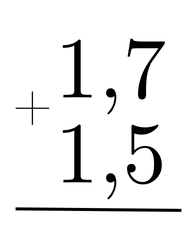
\includegraphics[width=0.15\linewidth]{imagens/decimal_1_7_1_5_1.png}
        \label{fig:decimal_1_7_1_5_1}
    \end{figure}

    E a partir daí resolvemos como se fosse uma soma como qualquer outra, como vimos no capítulo de adição.
    
    \begin{figure}[H]
        \centering
        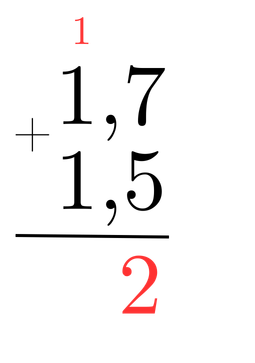
\includegraphics[width=0.2\linewidth]{imagens/decimal_1_7_1_5_2.png}
        \label{fig:decimal_1_7_1_5_2}
    \end{figure}

    \begin{figure}[H]
        \centering
        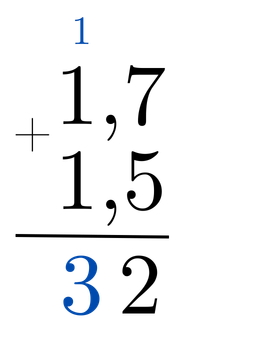
\includegraphics[width=0.2\linewidth]{imagens/decimal_1_7_1_5_3.png}
        \label{fig:decimal_1_7_1_5_3}
    \end{figure}

    Ao final, ``descemos'' a vírgula para baixo da linha também
    \begin{figure}[H]
        \centering
        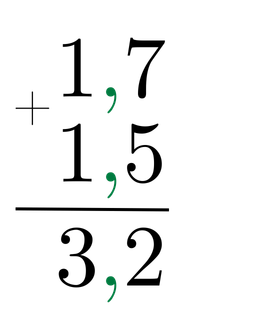
\includegraphics[width=0.2\linewidth]{imagens/decimal_1_7_1_5_4.png}
        \label{fig:decimal_1_7_1_5_4}
    \end{figure}
\end{exemplo}

\begin{exemplo}
    Considere a soma de 23,4 e 0,64.

    \begin{figure}[H]
        \centering
        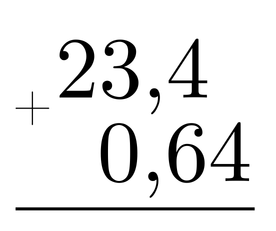
\includegraphics[width=0.2\linewidth]{imagens/decimal_23_4_0_64_1.png}
        \label{fig:decimal_23_4_0_64_1}
    \end{figure}
    Vírgula abaixo de vírgula, e temos uma coisa estranha: está ``faltando'' algarismo na parte de cima. Sem problema, nesses casos podemos preencher com o dígito 0 sem alterar o valor do número.
    
    \begin{figure}[H]
        \centering
        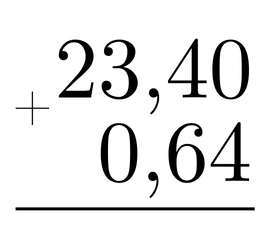
\includegraphics[width=0.2\linewidth]{imagens/decimal_23_4_0_64_2.png}
        \label{fig:decimal_23_4_0_64_2}
    \end{figure}

    E agora continuamos nossa soma da mesma maneira de sempre.
    
    \begin{figure}[H]
        \centering
        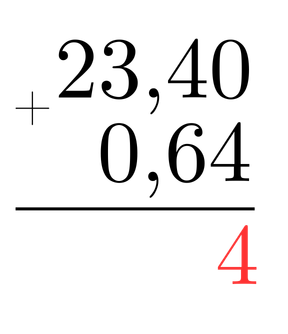
\includegraphics[width=0.2\linewidth]{imagens/decimal_23_4_0_64_3.png}
        \label{fig:decimal_23_4_0_64_3}
    \end{figure}

    \begin{figure}[H]
        \centering
        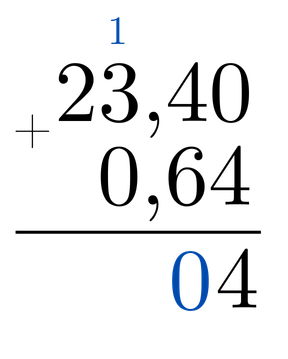
\includegraphics[width=0.2\linewidth]{imagens/decimal_23_4_0_64_4.png}
        \label{fig:decimal_23_4_0_64_4}
    \end{figure}

    \begin{figure}[H]
        \centering
        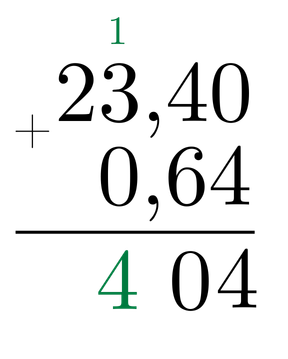
\includegraphics[width=0.2\linewidth]{imagens/decimal_23_4_0_64_5.png}
        \label{fig:decimal_23_4_0_64_5}
    \end{figure}

    \begin{figure}[H]
        \centering
        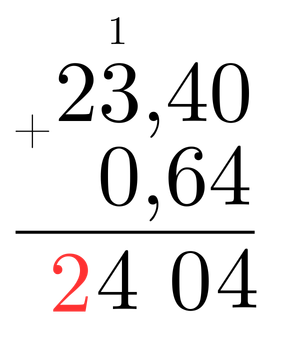
\includegraphics[width=0.2\linewidth]{imagens/decimal_23_4_0_64_6.png}
        \label{fig:decimal_23_4_0_64_6}
    \end{figure}

    Novamente, ao final ``descemos'' a vírgula e temos nosso resultado decimal.
    
    \begin{figure}[H]
        \centering
        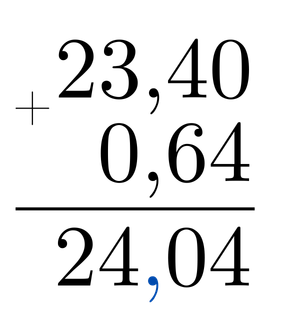
\includegraphics[width=0.2\linewidth]{imagens/decimal_23_4_0_64_7.png}
        \label{fig:decimal_23_4_0_64_7}
    \end{figure}

    \textcolor{red}{Obs.:} É importante que os números sejam posicionados corretamente no início exatamente para que o resultado também tenha a vírgula no lugar certo.
\end{exemplo}

E como já era de se esperar, o procedimento para realizar subtrações também será da mesma maneira que já vimos.

\begin{exemplo}

    Considere a subtração de 52,7 por 3,5.
    
    \begin{figure}[H]
        \centering
        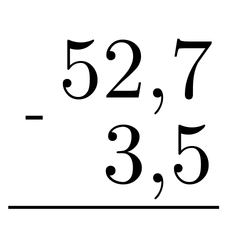
\includegraphics[width=0.2\linewidth]{imagens/decimal_52_7_3_5_1.png}
        \label{fig:decimal_52_7_3_5_1}
    \end{figure}

    \begin{figure}[H]
        \centering
        
\includegraphics[width=0.2\linewidth]{imagens/decimal_52_7_3_5_2.png}
        \label{fig:decimal_52_7_3_5_2}
    \end{figure}

    \begin{figure}[H]
        \centering
        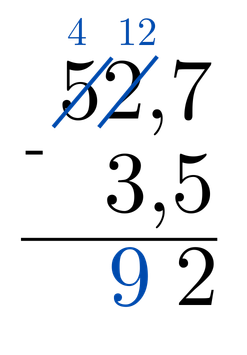
\includegraphics[width=0.2\linewidth]{imagens/decimal_52_7_3_5_3.png}
        \label{fig:decimal_52_7_3_5_3}
    \end{figure}

    \begin{figure}[H]
        \centering
        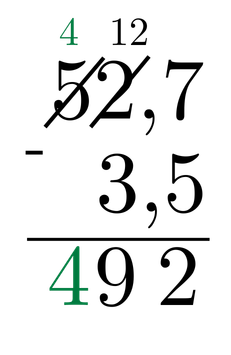
\includegraphics[width=0.2\linewidth]{imagens/decimal_52_7_3_5_4.png}
        \label{fig:decimal_52_7_3_5_4}
    \end{figure}

    \begin{figure}[H]
        \centering
        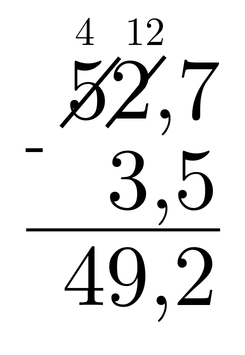
\includegraphics[width=0.2\linewidth]{imagens/decimal_52_7_3_5_5.png}
        \label{fig:decimal_52_7_3_5_5}
    \end{figure}
\end{exemplo}

Um último exemplo.

\begin{exemplo}
    Considere a subtração de 3,5 por 0,007.

    \begin{figure}[H]
        \centering
        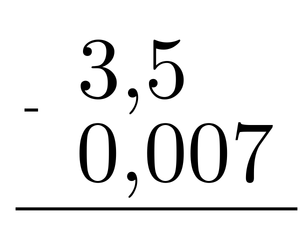
\includegraphics[width=0.2\linewidth]{imagens/decimal_3_5_0_007_1.png}
        \label{fig:decimal_3_5_0_007_1}
    \end{figure}

    Novamente, o número de cima parece estar ``faltando'' algarismos, mas vamos completar com zeros.

    \begin{figure}[H]
        \centering
        
\includegraphics[width=0.2\linewidth]{imagens/decimal_3_5_0_007_2.png}
        \label{fig:decimal_3_5_0_007_2}
    \end{figure}

    \begin{figure}[H]
        \centering
        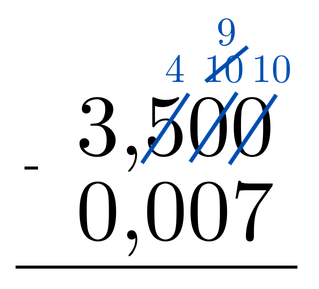
\includegraphics[width=0.2\linewidth]{imagens/decimal_3_5_0_007_3.png}
        \label{fig:decimal_3_5_0_007_3}
    \end{figure}

    \begin{figure}[H]
        \centering
        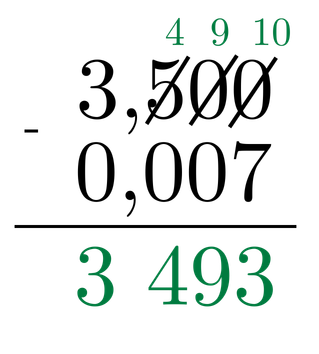
\includegraphics[width=0.2\linewidth]{imagens/decimal_3_5_0_007_4.png}
        \label{fig:decimal_3_5_0_007_4}
    \end{figure}

    \begin{figure}[H]
        \centering
        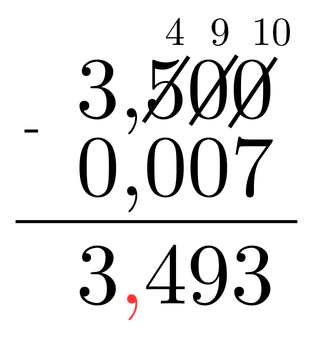
\includegraphics[width=0.2\linewidth]{imagens/decimal_3_5_0_007_5.png}
        \label{fig:decimal_3_5_0_007_5}
    \end{figure}
    
\end{exemplo}

E poderíamos ficar o resto da apostila aqui tirando exemplos mirabolantes, mas você já percebeu que não temos nada de novo até agora, somente posicionar as vírgulas corretamente e correr para o abraço.

\subsubsection{MULTIPLICAÇÃO E DIVISÃO DE DECIMAIS FINITOS}

Já para multiplicação de número decimais, temos um \textit{segredinho} que vai nos ajudar bastante. Agora, não precisamos mais nos preocupar em posicionar a vírgula corretamente abaixo da outra, o que vamos fazer é o seguinte: \textbf{ignorar que existem vírgulas}. 

Na verdade, não ignorar completamente, mas sim \textbf{contar} quantas casas decimais existem em cada número, somar essas quantidades e o resultado será exatamente a quantidade de casas decimais que o produto final deve ter. Vejamos um exemplo para ficar mais claro.

\begin{exemplo}
    Considere a multiplicação entre 12,35 e 0,4.

    \begin{figure}[H]
        \centering
        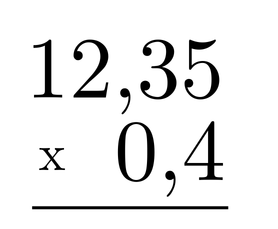
\includegraphics[width=0.2\linewidth]{imagens/decimal_12_35_0_4_1.png}
        \label{fig:decimal_12_35_0_4_1}
    \end{figure}

    Perceba que as vírgulas não estão alinhadas mais, pois isso não fará diferença. Primeiro, vamos anotar que 12,35 tem \textbf{duas} casas decimais e 0,4 tem \textbf{uma} casa decimal, ou seja, um total de \textbf{três} casas decimais - guarde essa informação. Agora, vamos ``fingir'' que essas vírgulas não existem:

    \begin{figure}[H]
        \centering
        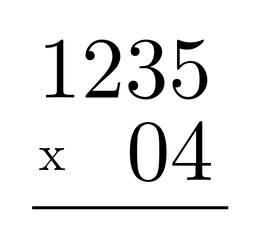
\includegraphics[width=0.2\linewidth]{imagens/decimal_12_35_0_4_2.png}
        \label{fig:decimal_12_35_0_4_2}
    \end{figure}

    E pronto, podemos realizar essa multiplicação da mesma forma que realizamos todas as outras anteriormente. Vamos fazer de maneira mais direta para economizar espaço, qualquer dúvida nessa parte retorne ao capítulo de multiplicação para revisão.

    \begin{figure}[H]
        \centering
        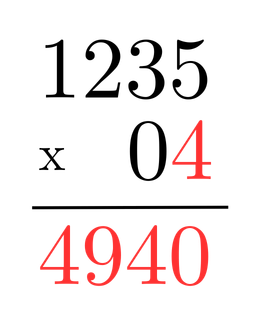
\includegraphics[width=0.2\linewidth]{imagens/decimal_12_35_0_4_3.png}
        \label{fig:decimal_12_35_0_4_3}
    \end{figure}

    E aqui vamos fingir que multiplicar por zero faz alguma diferença, só pelos velhos tempos. Mas fique atendo, pois se tivesse mais algarismos à esquerda do zero ai sim ele faria diferença.
    
    \begin{figure}[H]
        \centering
        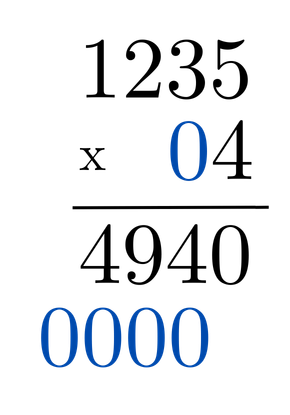
\includegraphics[width=0.2\linewidth]{imagens/decimal_12_35_0_4_4.png}
        \label{fig:decimal_12_35_0_4_4}
    \end{figure}

    \begin{figure}[H]
        \centering
        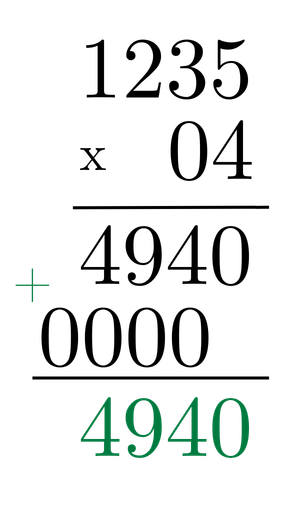
\includegraphics[width=0.2\linewidth]{imagens/decimal_12_35_0_4_5.png}
        \label{fig:decimal_12_35_0_4_5}
    \end{figure}

    \begin{figure}[H]
        \centering
        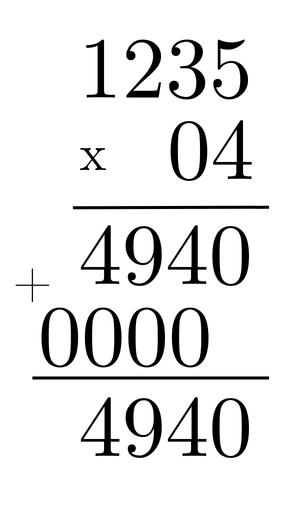
\includegraphics[width=0.2\linewidth]{imagens/decimal_12_35_0_4_6.png}
        \label{fig:decimal_12_35_0_4_6}
    \end{figure}

    E aqui entra o nosso truque: lembra no início do problema que encontramos que o produto final deveria ter 3 casas decimais? Pois então, agora é só andar com a vírgula 3 casas da direita para esquerda e temos o resultado decimal.
    
    \begin{figure}[H]
        \centering
        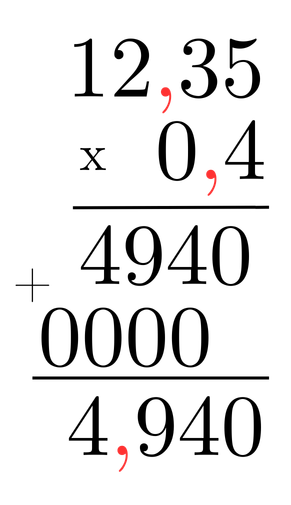
\includegraphics[width=0.2\linewidth]{imagens/decimal_12_35_0_4_7.png}
        \label{fig:decimal_12_35_0_4_7}
    \end{figure}
\end{exemplo}

Bem tranquilo, não é mesmo? Então a novidade para multiplicação de decimais é somente saber quantas casas decimais o produto final deve ter.

\begin{exemplo}
    Considere a multiplicação de 32,821 por 0,24.

    \begin{figure}[H]
        \centering
        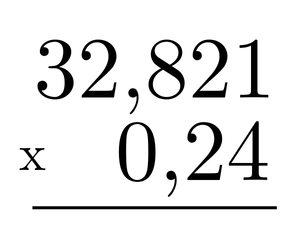
\includegraphics[width=0.2\linewidth]{imagens/decimal_32_821_0_24_1.png}
        \label{fig:decimal_32_821_0_24_1}
    \end{figure}

    Novamente, sabemos que 32,821 tem 3 casas decimais e 0,24 tem 2 casas decimais, então o produto final deve ter 5 casas decimais. E agora realizamos nossa conta normalmente.

    \begin{figure}[H]
        \centering
        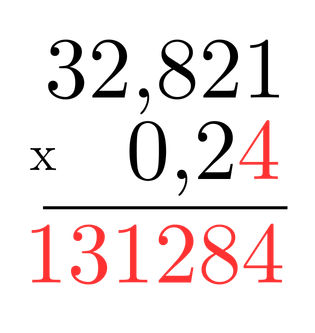
\includegraphics[width=0.2\linewidth]{imagens/decimal_32_821_0_24_2.png}
        \label{fig:decimal_32_821_0_24_2}
    \end{figure}

    \begin{figure}[H]
        \centering
        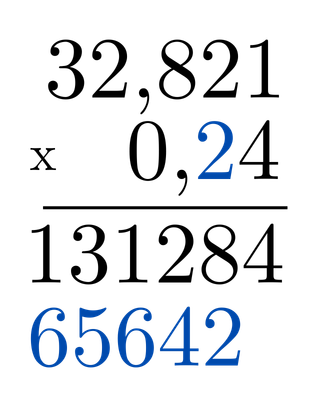
\includegraphics[width=0.2\linewidth]{imagens/decimal_32_821_0_24_3.png}
        \label{fig:decimal_32_821_0_24_3}
    \end{figure}
    
    \begin{figure}[H]
        \centering
        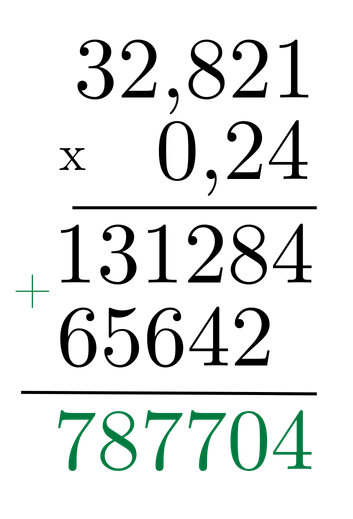
\includegraphics[width=0.2\linewidth]{imagens/decimal_32_821_0_24_4.png}
        \label{fig:decimal_32_821_0_24_4}
    \end{figure}

    Como o produto final deve ter 5 casas decimais, andamos com a vírgula 5 casas da direita para esquerda.

    \begin{figure}[H]
        \centering
        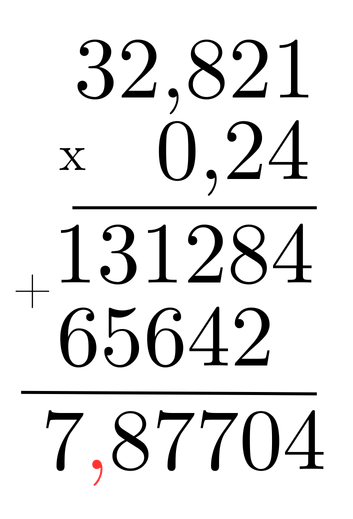
\includegraphics[width=0.2\linewidth]{imagens/decimal_32_821_0_24_5.png}
        \label{fig:decimal_32_821_0_24_5}
    \end{figure}
\end{exemplo}

Pronto, sem muitos segredos. Soma, subtração e multiplicação de decimais são processos relativamente simples, tão complexos quanto para números inteiros.

A maior ``dificuldade'' vem agora com \textbf{divisão de números decimais}. Mas não se assuste caro(a) aluno(a), pois também existem ``regrinhas'' a serem seguidas que vão facilitar bastante nossa vida e você nunca mais vai errar esse tipo de conta.


\begin{exemplo}
    Considere a divisão de 5 por 4.

    \begin{figure}[H]
        \centering
        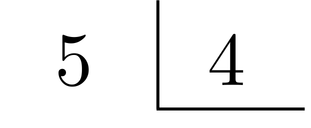
\includegraphics[width=0.3\linewidth]{imagens/decimais_5_4_1.png}
        \label{fig:decimais_5_4_1}
    \end{figure}

    Começamos nossa divisão como qualquer outra que já vimos até então:
    
    \begin{figure}[H]
        \centering
        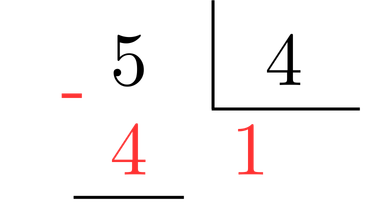
\includegraphics[width=0.35\linewidth]{imagens/decimais_5_4_2.png}
        \label{fig:decimais_5_4_2}
    \end{figure}
    
    \begin{figure}[H]
        \centering
        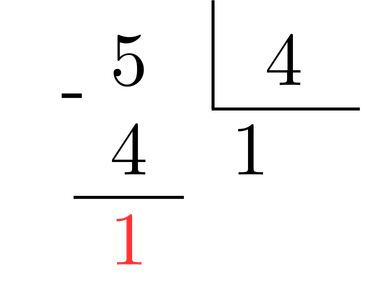
\includegraphics[width=0.35\linewidth]{imagens/decimais_5_4_3.png}
        \label{fig:decimais_5_4_3}
    \end{figure}
    
    E temos o resto 1. Até o momento nós aprendemos que ``devemos'' parar quando o resto for menor que o divisor, mas agora vamos aprender uma maneira que permita continuarmos essa divisão até encontrar um resto zero. 

    \vspace{0.5cm}

    \textbf{Primeiro}, adicionamos uma vírgula a direita do quociente para iniciarmos as casas decimais, e então adicionamos um algarismo \textbf{0} a direita do resto, transformando ele em \textbf{10}.
    
    \begin{figure}[H]
        \centering
        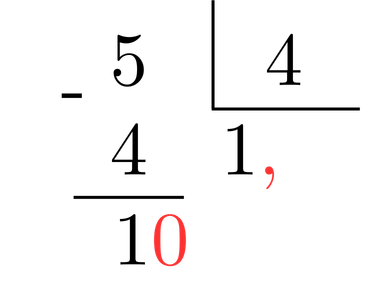
\includegraphics[width=0.35\linewidth]{imagens/decimais_5_4_4.png}
        \label{fig:decimais_5_4_4}
    \end{figure}

    A partir daí, continuamos nossa divisão como se nada tivesse acontecido.
    
    \begin{figure}[H]
        \centering
        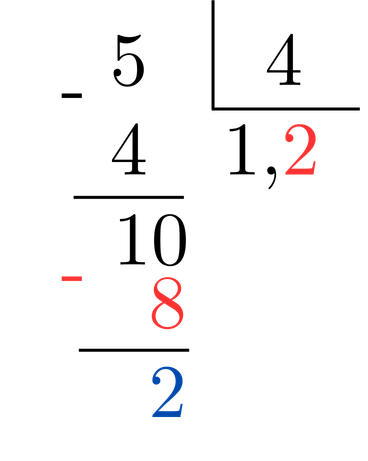
\includegraphics[width=0.35\linewidth]{imagens/decimais_5_4_5.png}
        \label{fig:decimais_5_4_5}
    \end{figure}

    No entanto, novamente caímos no problema do resto menor que o divisor\(\dots\) e isso acontecerá várias vezes em diversos problemas. A primeira vez que adicionamos uma vírgula no quociente, também adicionamos um zero no resto, mas a partir daí não podemos adicionar mais vírgulas, então o que devemos fazer?

    \vspace{0.5cm}

    Pense que a vírgula serve de ``pagamento'' para aquele primeiro zero que adicionamos, mas se você precisar de \textbf{mais um} ao longo do procedimento, ele fica ``por conta da casa''. Em outras palavras, podemos adicionar mais um zero nesse novo resto sem ter que alterar nada no quociente - desde que seja necessário apenas somente um.
    
    \begin{figure}[H]
        \centering
        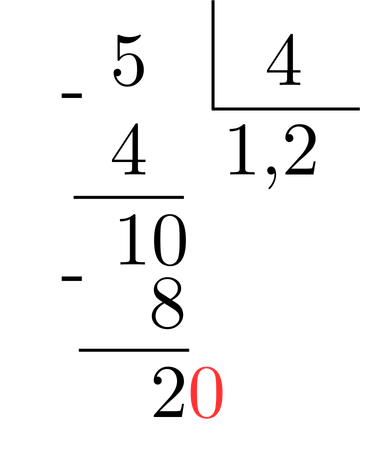
\includegraphics[width=0.35\linewidth]{imagens/decimais_5_4_6.png}
        \label{fig:decimais_5_4_6}
    \end{figure}

    E continuamos nossa divisão até obter o resto zero.
    
    \begin{figure}[H]
        \centering
        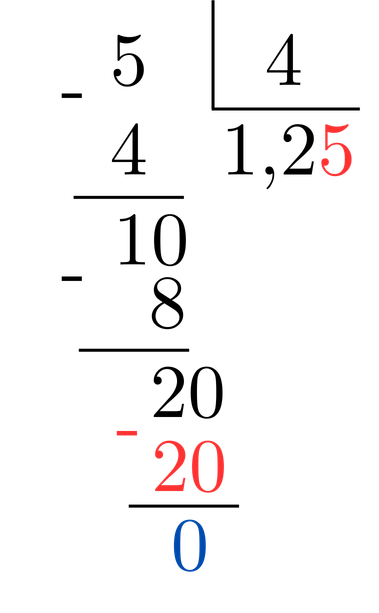
\includegraphics[width=0.35\linewidth]{imagens/decimais_5_4_7.png}
        \label{fig:decimais_5_4_7}
    \end{figure}

    Então, temos que o resultado da divisão de 5 por 4 é \textbf{1,25}.
\end{exemplo}

Vejamos agora um caso em que vamos precisar de adicionar mais zeros no resto em uma mesma etapa do processo de divisão.

\begin{exemplo}
    Considere a divisão de 3 por 60.

    \begin{figure}[H]
        \centering
        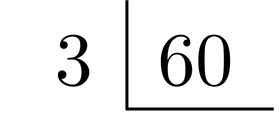
\includegraphics[width=0.28\linewidth]{imagens/decimais_3_60_1.png}
        \label{fig:decimais_3_60_1}
    \end{figure}

    Nesse caso agora já começamos a divisão com dividendo menor do que o divisor, mas podemos adicionar uma \textbf{vírgula no quociente} e um \textbf{zero no dividendo} (já que ainda não temos um resto).

    \begin{figure}[H]
        \centering
        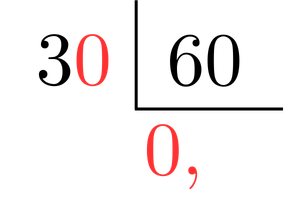
\includegraphics[width=0.3\linewidth]{imagens/decimais_3_60_2.png}
        \label{fig:decimais_3_60_2}
    \end{figure}

    No entanto, continuamos com um problema de dividendo menor que divisor, podemos adicionar mais um zero por conta da casa? Nesse caso, \textbf{não}, porque ainda estamos na mesma etapa da divisão (ainda com os mesmos números sendo divididos). Nesses casos em que tempos que pegar \textbf{dois ou mais} zeros ``emprestados'' para colocar no dividendo/resto, temos que adicionar a mesma quantidade de zeros no quociente. Veja:
    
    \begin{figure}[H]
        \centering
        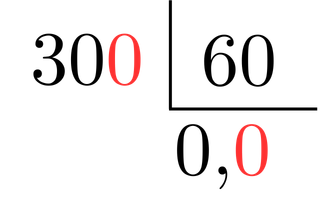
\includegraphics[width=0.3\linewidth]{imagens/decimais_3_60_3.png}
        \label{fig:decimais_3_60_3}
    \end{figure}

    Agora sim, temos o dividendo maior que o divisor e podemos realizar a próxima etapa da divisão.
    
    \begin{figure}[H]
        \centering
        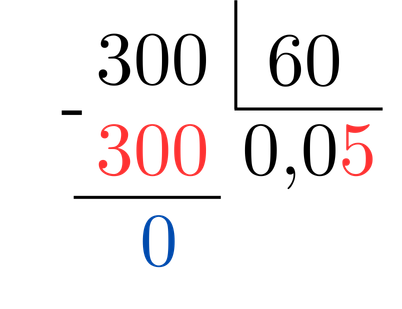
\includegraphics[width=0.35\linewidth]{imagens/decimais_3_60_4.png}
        \label{fig:decimais_3_60_4}
    \end{figure}

    Então, temos que a divisão de 3 por 60 é igual a \textbf{0,05}.
\end{exemplo}

\begin{exemplo}
    Considere a divisão de 2 por 8.

    \begin{figure}[H]
        \centering
        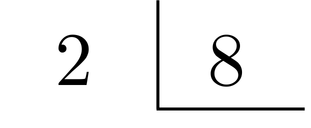
\includegraphics[width=0.3\linewidth]{imagens/decimais_2_8_1.png}
        \label{fig:decimais_2_8_1}
    \end{figure}

    Novamente começamos nossa divisão com dividendo menor que divisor, mas já sabemos que podemos adicionar uma vírgula no quociente e um zero no dividendo.
    
    \begin{figure}[H]
        \centering
        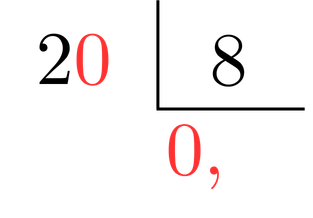
\includegraphics[width=0.3\linewidth]{imagens/decimais_2_8_2.png}
        \label{fig:decimais_2_8_2}
    \end{figure}
    
    \begin{figure}[H]
        \centering
        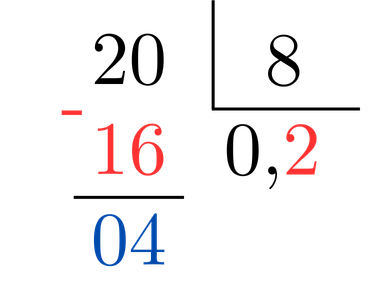
\includegraphics[width=0.35\linewidth]{imagens/decimais_2_8_3.png}
        \label{fig:decimais_2_8_3}
    \end{figure}

    Temos um resto menor que o divisor, mas podemos adicionar mais um zero ``por conta da casa'', já que estamos em uma \textbf{etapa diferente} da divisão.
    
    \textcolor{red}{Obs.:} Reflita bem se entendeu a diferença de quando podemos simplesmente adicionar mais um zero ou quando temos que adicionar também no quociente.
    \begin{figure}[H]
        \centering
        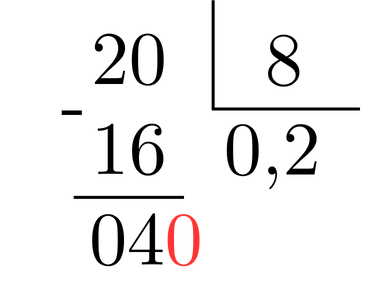
\includegraphics[width=0.35\linewidth]{imagens/decimais_2_8_4.png}
        \label{fig:decimais_2_8_4}
    \end{figure}

    \begin{figure}[H]
        \centering
        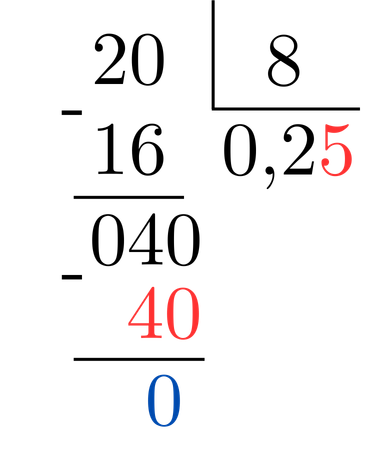
\includegraphics[width=0.35\linewidth]{imagens/decimais_2_8_5.png}
        \label{fig:decimais_2_8_5}
    \end{figure}

    Portanto, temos que a divisão de 2 por 8 é \textbf{0,25}.
\end{exemplo}

\begin{exemplo}
    Considere a divisão de 7,5 por 3.

    \begin{figure}[H]
        \centering
        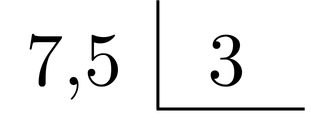
\includegraphics[width=0.3\linewidth]{imagens/decimais_7_5_3_1.png}
        \label{fig:decimais_7_5_3_1}
    \end{figure}

    E aqui temos uma \textit{novidade}: divisão de decimais por número inteiro. Nesse primeiro caso, podemos pensar essa divisão em forma de fração para ajudar a visualizar o processo.

    \begin{equation}
        7,5\div3 = \frac{7,5}{3}
    \end{equation}

    E em frações nós vimos que existem \textbf{frações equivalente}, ou seja, que possuem o mesmo valor mas estão escritas de forma ``diferente''. No nosso caso, vamos multiplicar por 10 em cima e em baixo da fração:

    \begin{equation}
        \frac{7,5}{3}\times\frac{10}{10} = \frac{75}{30}
    \end{equation}

    Que na prática não muda nada, pois estamos multiplicando por 1, mas que ajudou transformarmos uma divisão de decimais em uma divisão ``normal''. Sem ter que ficar transformando essas divisões para frações, vejamos como poderíamos fazer a \textbf{mesma coisa} diretamente no dispositivo prático.
    
    \begin{figure}[H]
        \centering
        
\includegraphics[width=0.3\linewidth]{imagens/decimais_7_5_3_2.png}
        \label{fig:decimais_7_5_3_2}
    \end{figure}

    Nesse caso, andamos com a vírgula uma casa para direita no dividendo e uma casa para direita no divisor (adicionando um zero pois ele não era decimal). Isso é equivalente a multiplicar as frações por 10 em cima e em baixo, e sempre vamos querer fazer isso para eliminar as casas decimais tanto do divisor quanto dividendo.
    
    \begin{figure}[H]
        \centering
        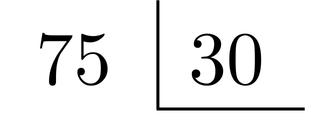
\includegraphics[width=0.3\linewidth]{imagens/decimais_7_5_3_3.png}
        \label{fig:decimais_7_5_3_3}
    \end{figure}

    E agora fazemos nossa divisão normalmente, sem novidades do que já vimos.
    
    \begin{figure}[H]
        \centering
        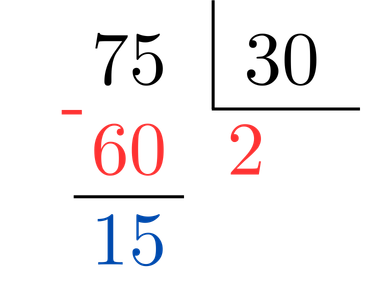
\includegraphics[width=0.35\linewidth]{imagens/decimais_7_5_3_4.png}
        \label{fig:decimais_7_5_3_4}
    \end{figure}

    \begin{figure}[H]
        \centering
        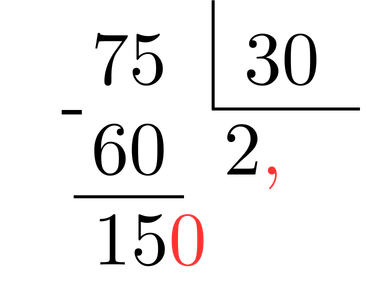
\includegraphics[width=0.35\linewidth]{imagens/decimais_7_5_3_5.png}
        \label{fig:decimais_7_5_3_5}
    \end{figure}

    \begin{figure}[H]
        \centering
        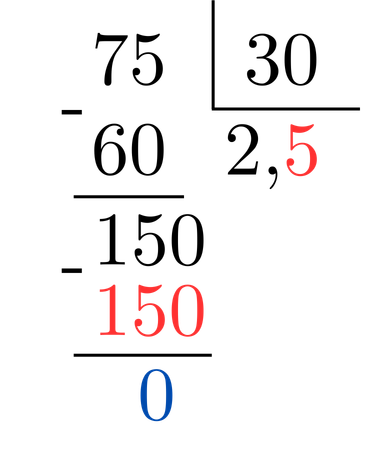
\includegraphics[width=0.35\linewidth]{imagens/decimais_7_5_3_6.png}
        \label{fig:decimais_7_5_3_6}
    \end{figure}

    Portanto, a divisão de 7,5 por 3 é \textbf{2,5}.
\end{exemplo}

\begin{exemplo}
    Considere a divisão de 3,6 por 0,12.

    \begin{figure}[H]
        \centering
        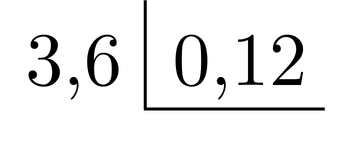
\includegraphics[width=0.35\linewidth]{imagens/decimais_3_6_0_12_1.png}
        \label{fig:decimais_3_6_0_12_1}
    \end{figure}

    Da mesma maneira que fizemos para o exemplo anterior, vamos multiplicar por 10 sucessivas vezes até que todos os decimais tenham ``desaparecido''
    \begin{figure}[H]
        \centering
        
\includegraphics[width=0.35\linewidth]{imagens/decimais_3_6_0_12_2.png}
        \label{fig:decimais_3_6_0_12_2}
    \end{figure}

    \begin{figure}[H]
        \centering
        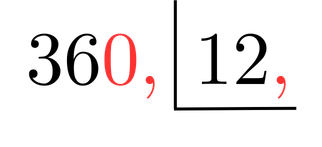
\includegraphics[width=0.35\linewidth]{imagens/decimais_3_6_0_12_3.png}
        \label{fig:decimais_3_6_0_12_3}
    \end{figure}

    Só relembrando que 012 é a mesma coisa que 12. Como não temos mais decimais, podemos começar o nosso processo de divisão.
    
    \begin{figure}[H]
        \centering
        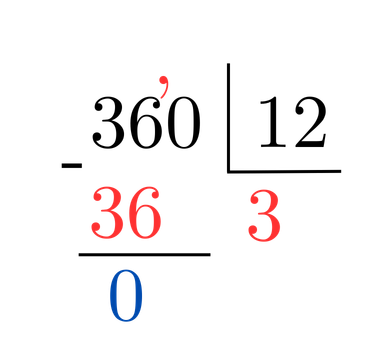
\includegraphics[width=0.35\linewidth]{imagens/decimais_3_6_0_12_4.png}
        \label{fig:decimais_3_6_0_12_4}
    \end{figure}

    \begin{figure}[H]
        \centering
        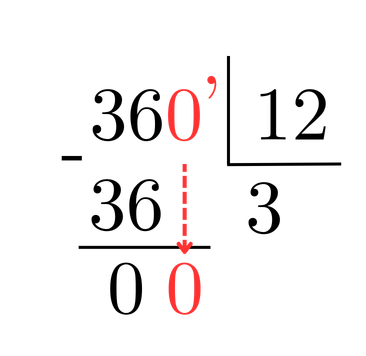
\includegraphics[width=0.35\linewidth]{imagens/decimais_3_6_0_12_5.png}
        \label{fig:decimais_3_6_0_12_5}
    \end{figure}

    \begin{figure}[H]
        \centering
        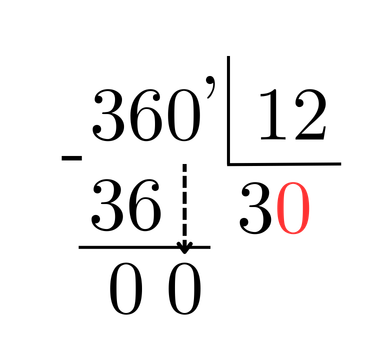
\includegraphics[width=0.35\linewidth]{imagens/decimais_3_6_0_12_6.png}
        \label{fig:decimais_3_6_0_12_6}
    \end{figure}

    Portanto, a divisão de 3,6 por 0,12 é \textbf{30}
\end{exemplo}

E nesse momento o(a) aluno(a) deve estar se perguntando: \textit{como a divisão de dois números pequenos pode dar um resultado muito maior do que eles?}. Pois então, esse é o \textit{poder} de realizarmos divisões por número muito pequenos, pois para ``eliminar'' as casas decimais temos que multiplicar por múltiplos de 10 cada vez maiores. Por curiosidade, pegue uma calculadora e divida 3 por 0,1, depois por 0,01, depois por 0,001 e assim em diante. O que acontece com o resultado a medida que reduzimos o divisor?

Vejamos agora um caso especial, em que vamos cair em uma dízima periódica (\textbf{decimal infinito periódico} na seção seguinte).

\begin{exemplo}
    Considere a divisão de 1 por 3.

    \begin{figure}[H]
        \centering
        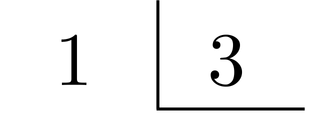
\includegraphics[width=0.3\linewidth]{imagens/decimais_1_3_1.png}
        \label{fig:decimais_1_3_1}
    \end{figure}

    \begin{figure}[H]
        \centering
        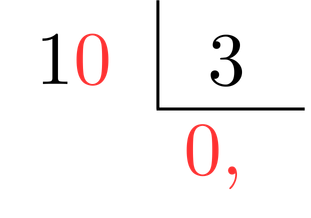
\includegraphics[width=0.3\linewidth]{imagens/decimais_1_3_2.png}
        \label{fig:decimais_1_3_2}
    \end{figure}

    \begin{figure}[H]
        \centering
        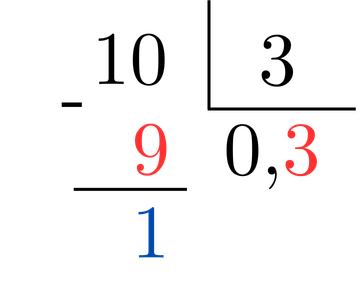
\includegraphics[width=0.35\linewidth]{imagens/decimais_1_3_3.png}
        \label{fig:decimais_1_3_3}
    \end{figure}

    \begin{figure}[H]
        \centering
        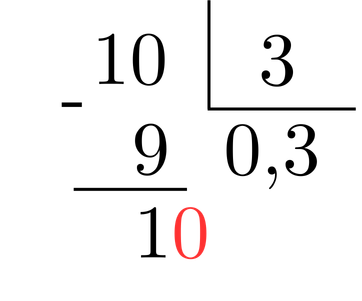
\includegraphics[width=0.35\linewidth]{imagens/decimais_1_3_4.png}
        \label{fig:decimais_1_3_4}
    \end{figure}

    \begin{figure}[H]
        \centering
        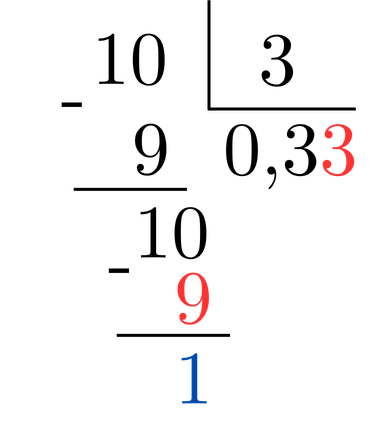
\includegraphics[width=0.35\linewidth]{imagens/decimais_1_3_5.png}
        \label{fig:decimais_1_3_5}
    \end{figure}

    E perceba que caímos em um \textit{loop}, pois sempre teremos um resto 1, que adicionando um zero a direita vai seguir para uma divisão de resto 1 novamente. Nesses casos, o quociente terá \textbf{infinitas} casas decimais, e não precisamos calcular até o infinito para perceber isso.

    \vspace{0,5cm}

    Porém, é um bom exemplo para mostrar que em \textbf{etapas diferentes} da divisão, podemos sempre adicionar um zero no resto sem ter que adicionar no quociente, infinitamente se necessário.
\end{exemplo}

\subsubsection{TRANSFORMAÇÃO DE DECIMAIS FINITOS PARA FRAÇÕES}
Esses números também são possíveis de serem reescritos em forma de fração, que pode acabar nos ajudando a resolver alguma operação de maneira mais fácil. Para isso, perceba que é só uma \textit{brincadeira} de movimentar a vírgula para esquerda ou direita até que não exista mais parte decimal. Vamos fazer isso dividindo ou multiplicando várias vezes por 10.

\begin{exemplo}
    Transforme o número 10,345 em fração.

    \vspace{0.5cm}

    Como podemos observar, existem três algarismos na parte decimal desse número, ou seja, três algarismos depois da vírgula. Dessa forma, precisaríamos mover essa vírgula 3 casas para direita, até desaparecer com a parte decimal antes de transformá-lo em fração. Para isso, precisamos multiplicar três vezes por 10, ou seja, \(10,345\times10\times10\times10\) que é a mesma coisa que multiplicá-lo por 1000.

    \begin{equation}
        10,345\times10=103,45
    \end{equation}
    \begin{equation}
        103,45\times10=1034,5
    \end{equation}
    \begin{equation}
        1034,5\times10=10345
    \end{equation}

    E pronto, \textit{destruímos} a parte decimal do número. Porém, é de se esperar que 10,345 seja \textbf{diferente} de 10345, e eles de fato não são o mesmo número, nem equivalentes. Portanto, violamos uma premissa fundamental da matemática que é ``não causarás nenhum mal''... \textit{ou isso é de outro lugar}? 

    \vspace{0.5cm}

    De qualquer forma, não podemos alterar o valor de um número como bem entendermos, ou tudo vira bagunça. Por isso, da mesma forma que multiplicamos ele três vezes por 10, ou seja por 1000, também devemos dividir ele por 1000, pois dessa maneira teremos:

    \begin{equation}
        10,345\times\frac{1000}{1000}=10,345\times1=10,345
    \end{equation}

    Novamente, estaremos usando a propriedade do elemento neutro da multiplicação, que é o 1, pois todo número multiplicado por 1 é ele mesmo. Ora, então se fizermos isso não estaremos alterando o valor do número. Então:

    \begin{equation}
        \frac{10,345\times1000}{1000}
    \end{equation}

    também não alteraria o valor do número, e eu não seria punido por isso. Mas nós também vimos que \(10,345\times1000=10345\). Vejamos:

    \begin{equation}
        \frac{10,345\times1000}{1000}=\frac{10345}{1000}
    \end{equation}

    E... fim? Encontramos o número na forma de fração? De certa forma, \textbf{sim}! Teríamos ainda que simplificar para que ele se torne a menor fração possível - irredutível.
\end{exemplo}

\begin{tcolorbox}[title=IMPORTANTE]
    Um pouco mais formalmente, iremos transformar decimais em frações multiplicando e dividindo o número por \textbf{múltiplos} de 10 (10, 100, 1000 etc), que dá na mesma que multiplicar e dividir por 10 várias vezes. No entanto, o conceito de múltiplos será apresentado mais pra frente na apostila. 
\end{tcolorbox}

\begin{exemplo}
    Transforme 0,025 para fração:

    \begin{equation}
        0,025=0,025\times\frac{1000}{1000}=\frac{25}{1000}
    \end{equation}

    A princípio poderíamos parar por ai e dizer que 0,025 é equivalente a 25/1000 em forma de fração, mas como já aprendemos a simplificar frações, vamos finalizar simplificando por 25 no numerador e denominador:

    \begin{equation}
        \frac{25}{1000}=\frac{1}{40}
    \end{equation}

    Agora sim, podemos dizer de maneira mais adequada que a forma de fração de 0,025 é 1/40.
\end{exemplo}







\subsection{Decimais infinitos periódicos}

Decimais infinitos periódicos é somente um nome bonito para \textbf{dízimas periódicas}. Não sabe o que é uma dízima periódica? Pegue uma calculadora qualquer e realize a divisão (razão) entre 1 e 3, ou seja, calcule o valor de 1/3 (um terço).

Dízimas periódicas sempre vão ter um conjunto de um ou mais algarismos se repetindo infinitamente. No caso de 1/3, que tem resultado 0,333333... teremos que o algarismo 3 se repete infinitamente. ``Ah, mas a minha calculadora não ficou digitando 3 infinitamente e parou alguns algarismos depois'', exatamente, que perspicaz... e de fato não faz sentido sua calculadora tentar representar pra você a mesma coisa que vai ser \textit{imutável} até o infinito, além de que ela teria que ficar calculando e te mostrando até a bateria acabar. 

Por isso, costumamos representar dízimas periódicas colocando uma ``barra'' em cima dos algarismos que vão se repetir infinitamente. Por exemplo, podemos escrever que \(1/3=0,3333\dots=0,\bar{3}\), sendo essa barra em cima do três uma representação de que ele repete indefinidamente.

Vejamos outro exemplo, agora digite na sua calculadora a razão 1/6 (um sexto), você encontrá algo como \(0,166666\dots\), que agora podemos representar como \(0,1\bar{6}\), pois somente o algarismo 6 se repete. É comum que algumas calculadoras mostrem algo como ``0,16666666667'' (ou algo parecido com isso), que acontece porque ela tenta arredondar o último algarismo que é capaz de te mostrar, mas continuaria sendo o algarismo 6 até o infinito.

Caso o(a) aluno(a) tente realizar alguma dessas divisões na caneta e papel, utilizando o dispositivo prático de divisão que vimos, ele(a) iria perceber que sempre irá sobrar um \textbf{resto} nessas divisões, por isso o processo se torna infinito.

Vamos ver mais alguns exemplos de dízimas periódicas.

\begin{exemplo}
    Considere a razão 2/3 (dois terços).

    \vspace{0.5cm}

    É uma divisão que também nos dá uma dízima periódica \(2,3333333\dots\), então podemos escrevê-la como \(2,\bar{3}\).
\end{exemplo}

\begin{exemplo}
    Considere a razão 34/99 (trinta e quatro e noventa e nove avos).

    \vspace{0.5cm}

    Essa divisão agora nos dará uma dízima periódica um pouco diferente, algo como \(0,3434343434\dots\). Nesse caso, temos 2 algarismos repetindo infinitamente, ou podemos dizer que o número 34 se repete. Com isso, podemos escrever essa dízima como \(0,\overline{34}\).
\end{exemplo}

No exemplo anterior podemos perceber que nem sempre teremos somente 1 algarismo se repetindo infinitamente, podemos ter 2, 3, 4 ou mais. Nesses casos, dizemos que é uma dízima periódica de \textbf{período} 2 (ou 3, 4, 5 etc). Em outras palavras, o termo ``periódico'' diz respeito à qual o período de repetição daquela dízima, com o período correspondente à quantos algarismos estão sendo repetidos.

\begin{exemplo}
    Considere a razão 123/999 (cento e vinte e três e novecentos e noventa e nove avos).

    \begin{equation}
        \frac{123}{999}=0,123123123123\dots=0,\overline{123}
    \end{equation}
    
    Essa divisão nos fornece uma dízima de período 3, já que três algarismos se repetem.
\end{exemplo}

\subsubsection{DÍZIMAS PERIÓDICAS SIMPLES E COMPOSTAS}

Somente a título de informação, existem dizimas periódicas \textbf{simples}, quando existe somente a dízima na parte decimal (quase todos exemplos que vimos até agora), e \textbf{compostas}, quando existe algum outro algarismo na parte decimal que não faz parte da dízima (como vimos no caso de 1/6).

\begin{exemplo}
    Considere a dízima periódica \(3,57\overline{4}\).

    \vspace{0.5cm}

    Nesse caso, temos uma dízima periódica \textbf{composta} de período 1 (somente o 4 se repete), pois existem os algarismos 5 e 7 na parte decimal anterior à dízima.
\end{exemplo}

Nesse ponto o(a) estudante deve estar se perguntando ``Tá, entendi, mas ser simples ou composta faz diferença em que?'', o que seria uma indagação justa e válida. E a resposta para essa pergunta aparece quando tentamos transformar essas dízimas em frações, similarmente como tínhamos feito com os decimais finitos.

\subsubsection{TRANSFORMAÇÃO DE DÍZIMAS PERIÓDICAS EM FRAÇÕES}

Primeiramente, vamos aprender como transformar \textbf{dízimas periódicas simples} em frações. O(a) estudante atento(a) já deve ter percebido algo curioso em alguns exemplos anteriores, em que esse autor que vos fala utilizou razões \textit{estranhas} como: 34/99 e 123/999. E isso tem a ver exatamente com a maneira que transformamos essas dízimas em frações.

De maneira bem simplificada, no caso de dízimas periódicas simples temos somente que identificar qual é o período da dízima e dividir os algarismos que se repetem pela mesma quantidade de algarismos 9 (9, 99, 999, 9999 etc). Fim, só isso. Vejamos alguns exemplos para ajudar na visualização.

\begin{exemplo}
    Transforme a dízima periódica \(0,\overline{45}\) em fração.

    \vspace{0.5cm}

    Nesse caso, temos uma dízima periódica simples de período 2, ou seja, temos que dividir os algarismos que se repetem por 99:

    \begin{equation}
        0,\overline{45}=\frac{45}{99}
    \end{equation}

    Simples assim. Claro que temos que simplificar a fração para que ela se torne irredutível e tudo mais, mas o processo é só isso mesmo.
\end{exemplo}

\begin{exemplo}
    Transforme a dízima periódica \(0,\bar{3}\) em fração.

    \vspace{0.5cm}

    Nesse caso, temos uma dízima periódica simples de período 1, então é somente realizar a divisão por 9.
    
    \begin{equation}
        0,\bar{3}=\frac{3}{9}
    \end{equation}

    Que simplificando chegamos no nosso 1/3.
\end{exemplo}

\begin{exemplo}
    Transforme a dízima periódica \(0,\overline{5674}\) em fração.

    Novamente, temos uma dízima de período 4, então devemos dividi-la por 9999.

    \begin{equation}
        0,\overline{5674}=\frac{5674}{9999}
    \end{equation}

    E boa sorte para simplificar essa equação.
\end{exemplo}

Vejamos agora um caso um pouco diferente e mais interessante.

\begin{exemplo}
    Transforme a dízima periódica \(2,\overline{34}\) em fração.

    \vspace{0.5cm}

    Ainda temos uma dízima periódica simples, porém agora com uma parte inteira. O processo continua sendo praticamente o mesmo, com a diferença que temos que ``remover'' a parte inteira antes de executá-lo.

    \begin{equation}
        2,\overline{34}=2+0,\overline{34}
    \end{equation}

    E pronto, temos novamente a nossa dízima sozinha para realizar o procedimento.

    \begin{equation}
        2+0,\overline{34}=2+\frac{34}{99}
    \end{equation}

    Novamente, poderíamos parar por aqui, mas fica mais elegante escrevermos como uma única fração.

    \begin{equation}
        2+\frac{34}{99}=\frac{198+34}{99}=\frac{232}{99}
    \end{equation}

    E fim, agora é só simplificar se for necessário.

    \vspace{0.5cm}

    \textcolor{red}{Observação:} Caso algum(a) aluno(a) tenha ficado com dúvida no último passo, sugiro fortemente ler/reler o capítulo \ref{fracoes}.
\end{exemplo}

Existem outras maneiras também de se transformar dízimas periódicas simples com parte inteira em frações, mas essa apresentada é a mais direta. Vamos fazer um último exemplo, utilizando um método um \textit{pouquinho} diferente, mas que na verdade é a ``demonstração'' do nosso método antereior de se dividir por 9, 99, 999 etc.

\begin{tcolorbox}[title=IMPORTANTE]
    O próximo exemplo talvez só faça sentido se você já souber trabalhar com equações ou se já tiver lido o capítulo \ref{equacoes}. Se preferir, o(a) estudante pode pular esse exemplo e continuar a leitura do texto, retornando nele depois que estiver mais familiarizado com equações do primeiro grau.
\end{tcolorbox}

\begin{exemplo}
    Transforme a dízima periódica \(1,\overline{54}\) em fração.

    \vspace{0.5cm}

    E antes de começarmos, eu convido você a tentar resolver pelo método apresentado anteriormente antes de continuar lendo esse exemplo.

    \vspace{0.5cm}

    Vamos criar uma incógnita \(x\) para nos ajudar nesse método, e vamos fazer ela ter o valor exatamente da nossa dízima periódica.

    \begin{equation}
        x=1,5454545454\dots
    \end{equation}

    Como estamos trabalhando com uma \textbf{igualdade}, tudo que fizermos de um lado também devemos fazer do outro para que a igualdade permaneça verdadeira, certo?

    \begin{equation}
        100x=154,54545454\dots
    \end{equation}

    E aqui eu somente realizei a multiplicação por 100 nos dois lados. O motivo disso vai ficar mais claro logo a frente.

    \vspace{0.5cm}

    Como \(x=1,545454\dots\) e \(100x=154,545454\dots\), vou fazer a subtração de \(100x-x\), vamos ver o que acontece:

    \begin{equation}
        100x-x=154,545454\dots-1,545454\dots
    \end{equation}

    E nesse caso, como a parte decimal dos dois é igual (mesmo sendo uma dízima) a subtração delas vai dar um resultado zero. Veja:
    
    \begin{equation}
        99x=(154+0,545454\dots)-(1+0,545454\dots)
    \end{equation}

    \begin{equation}
        99x=154-1+\cancel{0,545454\dots}\cancel{-0,545454\dots}
    \end{equation}

    E resta somente:

    \begin{equation}
        99x=154-1
    \end{equation}

    \begin{equation}
        x=\frac{153}{99}
    \end{equation}

    Que se o(a) aluno(a) resolveu do método tradicional antes de chegar nesse resultado, vai conseguir perceber que obtivemos exatamente o mesmo valor no final.
\end{exemplo}

Agora sim nossa aventura começa de verdade, vamos ver como seria transformar \textbf{dízimas periódicas compostas} em frações. Da mesma forma do anterior, \textbf{esse método só vai fazer sentido se o(a) aluno(a) estiver familiarizado com equações do primeiro grau}. 

\begin{exemplo}
    Transforme a dízima periódica \(1,34\bar{5}\) em fração.

    \vspace{0.5cm}

    Diferente do que vimos até agora, temos algarismos na parte decimal que não fazem parte da dízima periódica (e também uma parte inteira). Como feito no exemplo anterior, vamos usar uma incógnita \(x\) para criar uma igualdade e nos ajudar com as contas.

    \begin{equation}
        x=1,3455555\dots
    \end{equation}

    Multiplicando por 100 dos dois lados nós obtemos:

    \begin{equation}
        100x=134,55555\dots
    \end{equation}

    Que é um resultado que ``deixa'' a dízima sozinha na parte decimal. Agora, vamos multiplicar o mesmo \(x\) por 1000:

    \begin{equation}
        1000x=1345,55555\dots
    \end{equation}

    E por que fazer isso? Similarmente ao exemplo anterior, agora podemos fazer \(1000x-100x\) para eliminar a dízima periódica do nosso problema. 

    \begin{equation}
        1000x-100x=1345,555\dots-134,555\dots
    \end{equation}

    Pulando alguns passos que já vimos mais detalhadamente no exemplo anterior:

    \begin{equation}
        900x=1345-134
    \end{equation}

    \begin{equation}
        900x=1211
    \end{equation}

    E por fim,

    \begin{equation}
        x=\frac{1211}{900}
    \end{equation}
\end{exemplo}

Parece mais complexo do que realmente é, e a prática leva à perfeição. A medida que realizarmos outros exercícios aplicando esses métodos, o processo se torna mais natural e menos complicado.


\subsection{Decimais infinitos não periódicos}

Felizmente, para número \textbf{decimais infinitos não periódicos} não teremos métodos mirabolantes de transformação em frações, muito menos iremos realizar operações com eles como vimos até então. Mas o que são essas majestosas criaturas? Primeiramente, são números com infinitas casas decimais e que \textbf{não apresentam um padrão de repetição}. 

Dentro do universo chamado Teoria dos Conjuntos, que não veremos aqui na nossa apostila, decimais infinitos não periódicos seriam o conjunto de números que chamamos de \textbf{Irracionais}. Mas o que isso significa? Exatamente, que eles não fazem parte do conjunto dos \textbf{Racionais}. Por nada.

O conjunto dos números racionais englobaria os nossos números decimais finitos e os infinitos periódicos, e o que eles tinham em comum? Precisamente, nós conseguíamos transformá-los em frações, enquanto que agora com os não periódicos nós ``não vamos conseguir''.

Por ora, basta saber que esses números Irracionais existem, e eles vão englobar os nossos números infinitos não periódicos. Vamos ver alguns exemplos:

\begin{itemize}
    \item \(\pi\approx 3,1415926535\dots\) (Pi)
    \item \(\sqrt{2}\approx 1,414213562373\dots\)
    \item \(e\approx2,71828\dots\) (número de Euler)
    \item \(\phi\approx1,61803398\dots\) (número de ouro / razão áurea)
\end{itemize}

E muitos outros. Interessante perceber que alguns desses números são tão famosos, ou geraram tanta curiosidade naqueles que os ``encontraram'', que eles até ganharam nomes.

Você estaria enganado de pensar que esses números não tem nenhuma utilidade, muito pelo contrário. O número \(\pi\), por exemplo, ``dita as regras'' quando estamos falando de circunferências e esferas, sendo também amplamente aplicado em criptografia moderna.

O número de Euler (lê-se ``Oiler'') é fundamental quando vamos conversar sobre matemática financeira, modelagem de crescimentos populacionais dentre várias outras aplicações. 

O número de ouro foi (e ainda é) muito admirado por aparecer em estruturas da natureza, como na disposição de sementes de girassol, conchas de caracóis (aproximadamente), pentagramas e pentágonos (figuras geométricas que vamos estudar em outra oportunidade).

A raiz de 2 também é um número cheio de ``segredos`` e superstições, existindo lendas de pessoas que foram mortas por revelarem certas características dele, sendo também a primeira raiz irracional ``descoberta''. Curiosamente, também é a razão entre altura e comprimento de uma folha tamanho A4 (teste você mesmo com uma régua) e fundamental para esse sistema de tamanhos.

E existem muitos outros números irracionais (decimais infinitos não periódicos), cada um com suas características excepcionais (ou não) e que valem nossa atenção. Não que os números precisem ter uma ``utilidade'' no nosso dia a dia, mas é conveniente quando podemos aplicá-los em algo.



\newpage
\section{Potenciação}
\label{potenciacao}
Imagine que queremos fazer a multiplicação de um número por ele mesmo diversas vezes, do tipo $N\times N\times N\times N\times N\times N\times N\times N$ (ou quantos mais N quisermos). Isso se torna um exemplo cotidiano quando estamos trabalhando com matemática financeira, por exemplo, em que temos que multiplicar um certo valor por uma taxa de juros diversas vezes ao longo de dias/meses/anos. Gastaríamos muito papel e caneta para escrever uma multiplicação desse tipo 30 vezes, por exemplo. Deve ter alguma maneira mais elegante. 

Outro exemplo (\textit{amaldiçoado}) que podemos pensar é uma pandemia, como foi a de COVID-19 no ano de 2020. Imagine que cada pessoa infectada seja capaz de infectar duas outras, chamamos isso de \textbf{fator R} (ou \(R_o\)). Então, no primeiro contágio seriam 2 novas pessoas infectadas, depois cada uma dessas infectaria outras 2, agora sendo 4, depois 8, depois 16, depois 32 e assim em diante. A cada novo contato o número de pessoas infectadas é dobrado, ou seja, é multiplicada por 2. Veja na Figura \ref{fig:cascata} uma parte desse processo.

\begin{figure}[H]
    \centering
    


\tikzset{every picture/.style={line width=0.75pt}} %set default line width to 0.75pt        

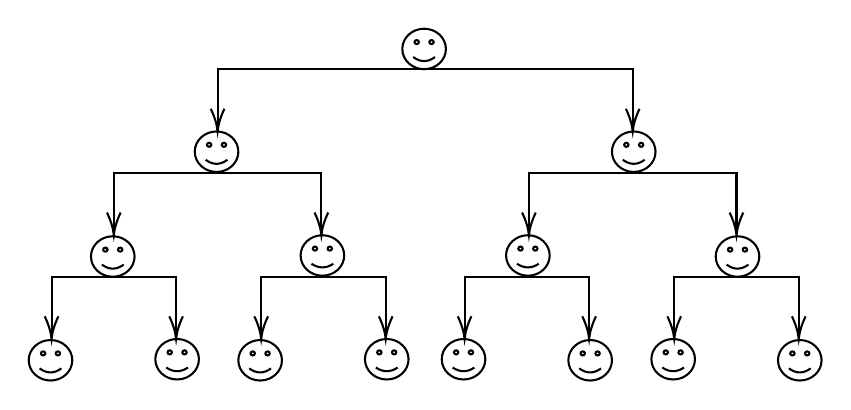
\begin{tikzpicture}[x=0.75pt,y=0.75pt,yscale=-1,xscale=1]
%uncomment if require: \path (0,300); %set diagram left start at 0, and has height of 300

%Straight Lines [id:da3889407615469902] 
\draw    (320,30) -- (220,30) -- (220,58) ;
\draw [shift={(220,60)}, rotate = 270] [color={rgb, 255:red, 0; green, 0; blue, 0 }  ][line width=0.75]    (10.93,-3.29) .. controls (6.95,-1.4) and (3.31,-0.3) .. (0,0) .. controls (3.31,0.3) and (6.95,1.4) .. (10.93,3.29)   ;
%Shape: Smiley Face [id:dp07527907239465303] 
\draw   (309,20.25) .. controls (309,14.87) and (313.7,10.5) .. (319.5,10.5) .. controls (325.3,10.5) and (330,14.87) .. (330,20.25) .. controls (330,25.63) and (325.3,30) .. (319.5,30) .. controls (313.7,30) and (309,25.63) .. (309,20.25) -- cycle ; \draw   (314.88,16.94) .. controls (314.88,16.4) and (315.35,15.96) .. (315.93,15.96) .. controls (316.51,15.96) and (316.98,16.4) .. (316.98,16.94) .. controls (316.98,17.47) and (316.51,17.91) .. (315.93,17.91) .. controls (315.35,17.91) and (314.88,17.47) .. (314.88,16.94) -- cycle ; \draw   (322.02,16.94) .. controls (322.02,16.4) and (322.49,15.96) .. (323.07,15.96) .. controls (323.65,15.96) and (324.12,16.4) .. (324.12,16.94) .. controls (324.12,17.47) and (323.65,17.91) .. (323.07,17.91) .. controls (322.49,17.91) and (322.02,17.47) .. (322.02,16.94) -- cycle ; \draw   (314.25,24.15) .. controls (317.75,26.75) and (321.25,26.75) .. (324.75,24.15) ;
%Shape: Smiley Face [id:dp44811925305118083] 
\draw   (209,69.75) .. controls (209,64.37) and (213.7,60) .. (219.5,60) .. controls (225.3,60) and (230,64.37) .. (230,69.75) .. controls (230,75.13) and (225.3,79.5) .. (219.5,79.5) .. controls (213.7,79.5) and (209,75.13) .. (209,69.75) -- cycle ; \draw   (214.88,66.44) .. controls (214.88,65.9) and (215.35,65.46) .. (215.93,65.46) .. controls (216.51,65.46) and (216.98,65.9) .. (216.98,66.44) .. controls (216.98,66.97) and (216.51,67.41) .. (215.93,67.41) .. controls (215.35,67.41) and (214.88,66.97) .. (214.88,66.44) -- cycle ; \draw   (222.02,66.44) .. controls (222.02,65.9) and (222.49,65.46) .. (223.07,65.46) .. controls (223.65,65.46) and (224.12,65.9) .. (224.12,66.44) .. controls (224.12,66.97) and (223.65,67.41) .. (223.07,67.41) .. controls (222.49,67.41) and (222.02,66.97) .. (222.02,66.44) -- cycle ; \draw   (214.25,73.65) .. controls (217.75,76.25) and (221.25,76.25) .. (224.75,73.65) ;
%Shape: Smiley Face [id:dp47067348664353736] 
\draw   (159,120.25) .. controls (159,114.87) and (163.7,110.5) .. (169.5,110.5) .. controls (175.3,110.5) and (180,114.87) .. (180,120.25) .. controls (180,125.63) and (175.3,130) .. (169.5,130) .. controls (163.7,130) and (159,125.63) .. (159,120.25) -- cycle ; \draw   (164.88,116.94) .. controls (164.88,116.4) and (165.35,115.96) .. (165.93,115.96) .. controls (166.51,115.96) and (166.98,116.4) .. (166.98,116.94) .. controls (166.98,117.47) and (166.51,117.91) .. (165.93,117.91) .. controls (165.35,117.91) and (164.88,117.47) .. (164.88,116.94) -- cycle ; \draw   (172.02,116.94) .. controls (172.02,116.4) and (172.49,115.96) .. (173.07,115.96) .. controls (173.65,115.96) and (174.12,116.4) .. (174.12,116.94) .. controls (174.12,117.47) and (173.65,117.91) .. (173.07,117.91) .. controls (172.49,117.91) and (172.02,117.47) .. (172.02,116.94) -- cycle ; \draw   (164.25,124.15) .. controls (167.75,126.75) and (171.25,126.75) .. (174.75,124.15) ;
%Shape: Smiley Face [id:dp6156820920337344] 
\draw   (260,119.75) .. controls (260,114.37) and (264.7,110) .. (270.5,110) .. controls (276.3,110) and (281,114.37) .. (281,119.75) .. controls (281,125.13) and (276.3,129.5) .. (270.5,129.5) .. controls (264.7,129.5) and (260,125.13) .. (260,119.75) -- cycle ; \draw   (265.88,116.44) .. controls (265.88,115.9) and (266.35,115.46) .. (266.93,115.46) .. controls (267.51,115.46) and (267.98,115.9) .. (267.98,116.44) .. controls (267.98,116.97) and (267.51,117.41) .. (266.93,117.41) .. controls (266.35,117.41) and (265.88,116.97) .. (265.88,116.44) -- cycle ; \draw   (273.02,116.44) .. controls (273.02,115.9) and (273.49,115.46) .. (274.07,115.46) .. controls (274.65,115.46) and (275.12,115.9) .. (275.12,116.44) .. controls (275.12,116.97) and (274.65,117.41) .. (274.07,117.41) .. controls (273.49,117.41) and (273.02,116.97) .. (273.02,116.44) -- cycle ; \draw   (265.25,123.75) .. controls (268.75,126.08) and (272.25,126.08) .. (275.75,123.75) ;
%Straight Lines [id:da45123805289386365] 
\draw    (220,80) -- (270,80) -- (270,108) ;
\draw [shift={(270,110)}, rotate = 270] [color={rgb, 255:red, 0; green, 0; blue, 0 }  ][line width=0.75]    (10.93,-3.29) .. controls (6.95,-1.4) and (3.31,-0.3) .. (0,0) .. controls (3.31,0.3) and (6.95,1.4) .. (10.93,3.29)   ;
%Straight Lines [id:da08913773098152444] 
\draw    (220,80) -- (170,80) -- (170,108) ;
\draw [shift={(170,110)}, rotate = 270] [color={rgb, 255:red, 0; green, 0; blue, 0 }  ][line width=0.75]    (10.93,-3.29) .. controls (6.95,-1.4) and (3.31,-0.3) .. (0,0) .. controls (3.31,0.3) and (6.95,1.4) .. (10.93,3.29)   ;
%Shape: Smiley Face [id:dp16632972448682848] 
\draw   (129,170.25) .. controls (129,164.87) and (133.7,160.5) .. (139.5,160.5) .. controls (145.3,160.5) and (150,164.87) .. (150,170.25) .. controls (150,175.63) and (145.3,180) .. (139.5,180) .. controls (133.7,180) and (129,175.63) .. (129,170.25) -- cycle ; \draw   (134.88,166.94) .. controls (134.88,166.4) and (135.35,165.96) .. (135.93,165.96) .. controls (136.51,165.96) and (136.98,166.4) .. (136.98,166.94) .. controls (136.98,167.47) and (136.51,167.91) .. (135.93,167.91) .. controls (135.35,167.91) and (134.88,167.47) .. (134.88,166.94) -- cycle ; \draw   (142.02,166.94) .. controls (142.02,166.4) and (142.49,165.96) .. (143.07,165.96) .. controls (143.65,165.96) and (144.12,166.4) .. (144.12,166.94) .. controls (144.12,167.47) and (143.65,167.91) .. (143.07,167.91) .. controls (142.49,167.91) and (142.02,167.47) .. (142.02,166.94) -- cycle ; \draw   (134.25,174.15) .. controls (137.75,176.75) and (141.25,176.75) .. (144.75,174.15) ;
%Shape: Smiley Face [id:dp7153536537365394] 
\draw   (190,169.75) .. controls (190,164.37) and (194.7,160) .. (200.5,160) .. controls (206.3,160) and (211,164.37) .. (211,169.75) .. controls (211,175.13) and (206.3,179.5) .. (200.5,179.5) .. controls (194.7,179.5) and (190,175.13) .. (190,169.75) -- cycle ; \draw   (195.88,166.44) .. controls (195.88,165.9) and (196.35,165.46) .. (196.93,165.46) .. controls (197.51,165.46) and (197.98,165.9) .. (197.98,166.44) .. controls (197.98,166.97) and (197.51,167.41) .. (196.93,167.41) .. controls (196.35,167.41) and (195.88,166.97) .. (195.88,166.44) -- cycle ; \draw   (203.02,166.44) .. controls (203.02,165.9) and (203.49,165.46) .. (204.07,165.46) .. controls (204.65,165.46) and (205.12,165.9) .. (205.12,166.44) .. controls (205.12,166.97) and (204.65,167.41) .. (204.07,167.41) .. controls (203.49,167.41) and (203.02,166.97) .. (203.02,166.44) -- cycle ; \draw   (195.25,173.75) .. controls (198.75,176.08) and (202.25,176.08) .. (205.75,173.75) ;
%Straight Lines [id:da7173246341247351] 
\draw    (169,130) -- (200,130) -- (200,158) ;
\draw [shift={(200,160)}, rotate = 270] [color={rgb, 255:red, 0; green, 0; blue, 0 }  ][line width=0.75]    (10.93,-3.29) .. controls (6.95,-1.4) and (3.31,-0.3) .. (0,0) .. controls (3.31,0.3) and (6.95,1.4) .. (10.93,3.29)   ;
%Straight Lines [id:da2890258177619984] 
\draw    (169,130) -- (140,130) -- (140,158) ;
\draw [shift={(140,160)}, rotate = 270] [color={rgb, 255:red, 0; green, 0; blue, 0 }  ][line width=0.75]    (10.93,-3.29) .. controls (6.95,-1.4) and (3.31,-0.3) .. (0,0) .. controls (3.31,0.3) and (6.95,1.4) .. (10.93,3.29)   ;
%Shape: Smiley Face [id:dp16647383241360536] 
\draw   (230,170.25) .. controls (230,164.87) and (234.7,160.5) .. (240.5,160.5) .. controls (246.3,160.5) and (251,164.87) .. (251,170.25) .. controls (251,175.63) and (246.3,180) .. (240.5,180) .. controls (234.7,180) and (230,175.63) .. (230,170.25) -- cycle ; \draw   (235.88,166.94) .. controls (235.88,166.4) and (236.35,165.96) .. (236.93,165.96) .. controls (237.51,165.96) and (237.98,166.4) .. (237.98,166.94) .. controls (237.98,167.47) and (237.51,167.91) .. (236.93,167.91) .. controls (236.35,167.91) and (235.88,167.47) .. (235.88,166.94) -- cycle ; \draw   (243.02,166.94) .. controls (243.02,166.4) and (243.49,165.96) .. (244.07,165.96) .. controls (244.65,165.96) and (245.12,166.4) .. (245.12,166.94) .. controls (245.12,167.47) and (244.65,167.91) .. (244.07,167.91) .. controls (243.49,167.91) and (243.02,167.47) .. (243.02,166.94) -- cycle ; \draw   (235.25,174.15) .. controls (238.75,176.75) and (242.25,176.75) .. (245.75,174.15) ;
%Shape: Smiley Face [id:dp783251269256997] 
\draw   (291,169.75) .. controls (291,164.37) and (295.7,160) .. (301.5,160) .. controls (307.3,160) and (312,164.37) .. (312,169.75) .. controls (312,175.13) and (307.3,179.5) .. (301.5,179.5) .. controls (295.7,179.5) and (291,175.13) .. (291,169.75) -- cycle ; \draw   (296.88,166.44) .. controls (296.88,165.9) and (297.35,165.46) .. (297.93,165.46) .. controls (298.51,165.46) and (298.98,165.9) .. (298.98,166.44) .. controls (298.98,166.97) and (298.51,167.41) .. (297.93,167.41) .. controls (297.35,167.41) and (296.88,166.97) .. (296.88,166.44) -- cycle ; \draw   (304.02,166.44) .. controls (304.02,165.9) and (304.49,165.46) .. (305.07,165.46) .. controls (305.65,165.46) and (306.12,165.9) .. (306.12,166.44) .. controls (306.12,166.97) and (305.65,167.41) .. (305.07,167.41) .. controls (304.49,167.41) and (304.02,166.97) .. (304.02,166.44) -- cycle ; \draw   (296.25,173.75) .. controls (299.75,176.08) and (303.25,176.08) .. (306.75,173.75) ;
%Straight Lines [id:da97123910241943] 
\draw    (270,130) -- (301,130) -- (301,158) ;
\draw [shift={(301,160)}, rotate = 270] [color={rgb, 255:red, 0; green, 0; blue, 0 }  ][line width=0.75]    (10.93,-3.29) .. controls (6.95,-1.4) and (3.31,-0.3) .. (0,0) .. controls (3.31,0.3) and (6.95,1.4) .. (10.93,3.29)   ;
%Straight Lines [id:da08661379201713204] 
\draw    (270,130) -- (241,130) -- (241,158) ;
\draw [shift={(241,160)}, rotate = 270] [color={rgb, 255:red, 0; green, 0; blue, 0 }  ][line width=0.75]    (10.93,-3.29) .. controls (6.95,-1.4) and (3.31,-0.3) .. (0,0) .. controls (3.31,0.3) and (6.95,1.4) .. (10.93,3.29)   ;
%Straight Lines [id:da6166210174766458] 
\draw    (320,30) -- (420,30) -- (420,58) ;
\draw [shift={(420,60)}, rotate = 270] [color={rgb, 255:red, 0; green, 0; blue, 0 }  ][line width=0.75]    (10.93,-3.29) .. controls (6.95,-1.4) and (3.31,-0.3) .. (0,0) .. controls (3.31,0.3) and (6.95,1.4) .. (10.93,3.29)   ;
%Shape: Smiley Face [id:dp4910895864122389] 
\draw   (431,69.75) .. controls (431,64.37) and (426.3,60) .. (420.5,60) .. controls (414.7,60) and (410,64.37) .. (410,69.75) .. controls (410,75.13) and (414.7,79.5) .. (420.5,79.5) .. controls (426.3,79.5) and (431,75.13) .. (431,69.75) -- cycle ; \draw   (425.12,66.44) .. controls (425.12,65.9) and (424.65,65.46) .. (424.07,65.46) .. controls (423.49,65.46) and (423.02,65.9) .. (423.02,66.44) .. controls (423.02,66.97) and (423.49,67.41) .. (424.07,67.41) .. controls (424.65,67.41) and (425.12,66.97) .. (425.12,66.44) -- cycle ; \draw   (417.98,66.44) .. controls (417.98,65.9) and (417.51,65.46) .. (416.93,65.46) .. controls (416.35,65.46) and (415.88,65.9) .. (415.88,66.44) .. controls (415.88,66.97) and (416.35,67.41) .. (416.93,67.41) .. controls (417.51,67.41) and (417.98,66.97) .. (417.98,66.44) -- cycle ; \draw   (425.75,73.65) .. controls (422.25,76.25) and (418.75,76.25) .. (415.25,73.65) ;
%Shape: Smiley Face [id:dp44371222182318026] 
\draw   (481,120.25) .. controls (481,114.87) and (476.3,110.5) .. (470.5,110.5) .. controls (464.7,110.5) and (460,114.87) .. (460,120.25) .. controls (460,125.63) and (464.7,130) .. (470.5,130) .. controls (476.3,130) and (481,125.63) .. (481,120.25) -- cycle ; \draw   (475.12,116.94) .. controls (475.12,116.4) and (474.65,115.96) .. (474.07,115.96) .. controls (473.49,115.96) and (473.02,116.4) .. (473.02,116.94) .. controls (473.02,117.47) and (473.49,117.91) .. (474.07,117.91) .. controls (474.65,117.91) and (475.12,117.47) .. (475.12,116.94) -- cycle ; \draw   (467.98,116.94) .. controls (467.98,116.4) and (467.51,115.96) .. (466.93,115.96) .. controls (466.35,115.96) and (465.88,116.4) .. (465.88,116.94) .. controls (465.88,117.47) and (466.35,117.91) .. (466.93,117.91) .. controls (467.51,117.91) and (467.98,117.47) .. (467.98,116.94) -- cycle ; \draw   (475.75,124.15) .. controls (472.25,126.75) and (468.75,126.75) .. (465.25,124.15) ;
%Shape: Smiley Face [id:dp598721335370733] 
\draw   (380,119.75) .. controls (380,114.37) and (375.3,110) .. (369.5,110) .. controls (363.7,110) and (359,114.37) .. (359,119.75) .. controls (359,125.13) and (363.7,129.5) .. (369.5,129.5) .. controls (375.3,129.5) and (380,125.13) .. (380,119.75) -- cycle ; \draw   (374.12,116.44) .. controls (374.12,115.9) and (373.65,115.46) .. (373.07,115.46) .. controls (372.49,115.46) and (372.02,115.9) .. (372.02,116.44) .. controls (372.02,116.97) and (372.49,117.41) .. (373.07,117.41) .. controls (373.65,117.41) and (374.12,116.97) .. (374.12,116.44) -- cycle ; \draw   (366.98,116.44) .. controls (366.98,115.9) and (366.51,115.46) .. (365.93,115.46) .. controls (365.35,115.46) and (364.88,115.9) .. (364.88,116.44) .. controls (364.88,116.97) and (365.35,117.41) .. (365.93,117.41) .. controls (366.51,117.41) and (366.98,116.97) .. (366.98,116.44) -- cycle ; \draw   (374.75,123.75) .. controls (371.25,126.08) and (367.75,126.08) .. (364.25,123.75) ;
%Straight Lines [id:da868852164013779] 
\draw    (420,80) -- (370,80) -- (370,108) ;
\draw [shift={(370,110)}, rotate = 270] [color={rgb, 255:red, 0; green, 0; blue, 0 }  ][line width=0.75]    (10.93,-3.29) .. controls (6.95,-1.4) and (3.31,-0.3) .. (0,0) .. controls (3.31,0.3) and (6.95,1.4) .. (10.93,3.29)   ;
%Straight Lines [id:da15151278762184106] 
\draw    (420,80) -- (470,80) -- (470,108) ;
\draw [shift={(470,110)}, rotate = 270] [color={rgb, 255:red, 0; green, 0; blue, 0 }  ][line width=0.75]    (10.93,-3.29) .. controls (6.95,-1.4) and (3.31,-0.3) .. (0,0) .. controls (3.31,0.3) and (6.95,1.4) .. (10.93,3.29)   ;
%Shape: Smiley Face [id:dp947008137961908] 
\draw   (511,170.25) .. controls (511,164.87) and (506.3,160.5) .. (500.5,160.5) .. controls (494.7,160.5) and (490,164.87) .. (490,170.25) .. controls (490,175.63) and (494.7,180) .. (500.5,180) .. controls (506.3,180) and (511,175.63) .. (511,170.25) -- cycle ; \draw   (505.12,166.94) .. controls (505.12,166.4) and (504.65,165.96) .. (504.07,165.96) .. controls (503.49,165.96) and (503.02,166.4) .. (503.02,166.94) .. controls (503.02,167.47) and (503.49,167.91) .. (504.07,167.91) .. controls (504.65,167.91) and (505.12,167.47) .. (505.12,166.94) -- cycle ; \draw   (497.98,166.94) .. controls (497.98,166.4) and (497.51,165.96) .. (496.93,165.96) .. controls (496.35,165.96) and (495.88,166.4) .. (495.88,166.94) .. controls (495.88,167.47) and (496.35,167.91) .. (496.93,167.91) .. controls (497.51,167.91) and (497.98,167.47) .. (497.98,166.94) -- cycle ; \draw   (505.75,174.15) .. controls (502.25,176.75) and (498.75,176.75) .. (495.25,174.15) ;
%Shape: Smiley Face [id:dp8721537645391825] 
\draw   (450,169.75) .. controls (450,164.37) and (445.3,160) .. (439.5,160) .. controls (433.7,160) and (429,164.37) .. (429,169.75) .. controls (429,175.13) and (433.7,179.5) .. (439.5,179.5) .. controls (445.3,179.5) and (450,175.13) .. (450,169.75) -- cycle ; \draw   (444.12,166.44) .. controls (444.12,165.9) and (443.65,165.46) .. (443.07,165.46) .. controls (442.49,165.46) and (442.02,165.9) .. (442.02,166.44) .. controls (442.02,166.97) and (442.49,167.41) .. (443.07,167.41) .. controls (443.65,167.41) and (444.12,166.97) .. (444.12,166.44) -- cycle ; \draw   (436.98,166.44) .. controls (436.98,165.9) and (436.51,165.46) .. (435.93,165.46) .. controls (435.35,165.46) and (434.88,165.9) .. (434.88,166.44) .. controls (434.88,166.97) and (435.35,167.41) .. (435.93,167.41) .. controls (436.51,167.41) and (436.98,166.97) .. (436.98,166.44) -- cycle ; \draw   (444.75,173.75) .. controls (441.25,176.08) and (437.75,176.08) .. (434.25,173.75) ;
%Straight Lines [id:da8109512192608107] 
\draw    (471,130) -- (440,130) -- (440,158) ;
\draw [shift={(440,160)}, rotate = 270] [color={rgb, 255:red, 0; green, 0; blue, 0 }  ][line width=0.75]    (10.93,-3.29) .. controls (6.95,-1.4) and (3.31,-0.3) .. (0,0) .. controls (3.31,0.3) and (6.95,1.4) .. (10.93,3.29)   ;
%Straight Lines [id:da0896745948919424] 
\draw    (471,130) -- (500,130) -- (500,158) ;
\draw [shift={(500,160)}, rotate = 270] [color={rgb, 255:red, 0; green, 0; blue, 0 }  ][line width=0.75]    (10.93,-3.29) .. controls (6.95,-1.4) and (3.31,-0.3) .. (0,0) .. controls (3.31,0.3) and (6.95,1.4) .. (10.93,3.29)   ;
%Shape: Smiley Face [id:dp7861164884235972] 
\draw   (410,170.25) .. controls (410,164.87) and (405.3,160.5) .. (399.5,160.5) .. controls (393.7,160.5) and (389,164.87) .. (389,170.25) .. controls (389,175.63) and (393.7,180) .. (399.5,180) .. controls (405.3,180) and (410,175.63) .. (410,170.25) -- cycle ; \draw   (404.12,166.94) .. controls (404.12,166.4) and (403.65,165.96) .. (403.07,165.96) .. controls (402.49,165.96) and (402.02,166.4) .. (402.02,166.94) .. controls (402.02,167.47) and (402.49,167.91) .. (403.07,167.91) .. controls (403.65,167.91) and (404.12,167.47) .. (404.12,166.94) -- cycle ; \draw   (396.98,166.94) .. controls (396.98,166.4) and (396.51,165.96) .. (395.93,165.96) .. controls (395.35,165.96) and (394.88,166.4) .. (394.88,166.94) .. controls (394.88,167.47) and (395.35,167.91) .. (395.93,167.91) .. controls (396.51,167.91) and (396.98,167.47) .. (396.98,166.94) -- cycle ; \draw   (404.75,174.15) .. controls (401.25,176.75) and (397.75,176.75) .. (394.25,174.15) ;
%Shape: Smiley Face [id:dp8645206701973079] 
\draw   (349,169.75) .. controls (349,164.37) and (344.3,160) .. (338.5,160) .. controls (332.7,160) and (328,164.37) .. (328,169.75) .. controls (328,175.13) and (332.7,179.5) .. (338.5,179.5) .. controls (344.3,179.5) and (349,175.13) .. (349,169.75) -- cycle ; \draw   (343.12,166.44) .. controls (343.12,165.9) and (342.65,165.46) .. (342.07,165.46) .. controls (341.49,165.46) and (341.02,165.9) .. (341.02,166.44) .. controls (341.02,166.97) and (341.49,167.41) .. (342.07,167.41) .. controls (342.65,167.41) and (343.12,166.97) .. (343.12,166.44) -- cycle ; \draw   (335.98,166.44) .. controls (335.98,165.9) and (335.51,165.46) .. (334.93,165.46) .. controls (334.35,165.46) and (333.88,165.9) .. (333.88,166.44) .. controls (333.88,166.97) and (334.35,167.41) .. (334.93,167.41) .. controls (335.51,167.41) and (335.98,166.97) .. (335.98,166.44) -- cycle ; \draw   (343.75,173.75) .. controls (340.25,176.08) and (336.75,176.08) .. (333.25,173.75) ;
%Straight Lines [id:da3199304666071091] 
\draw    (370,130) -- (339,130) -- (339,158) ;
\draw [shift={(339,160)}, rotate = 270] [color={rgb, 255:red, 0; green, 0; blue, 0 }  ][line width=0.75]    (10.93,-3.29) .. controls (6.95,-1.4) and (3.31,-0.3) .. (0,0) .. controls (3.31,0.3) and (6.95,1.4) .. (10.93,3.29)   ;
%Straight Lines [id:da12324697674665608] 
\draw    (370,130) -- (399,130) -- (399,158) ;
\draw [shift={(399,160)}, rotate = 270] [color={rgb, 255:red, 0; green, 0; blue, 0 }  ][line width=0.75]    (10.93,-3.29) .. controls (6.95,-1.4) and (3.31,-0.3) .. (0,0) .. controls (3.31,0.3) and (6.95,1.4) .. (10.93,3.29)   ;




\end{tikzpicture}

    \caption{Cascata de proliferação de uma certa doença com fator R = 2.}
    \label{fig:cascata}
\end{figure}

É muito comum ouvirmos dizer que esses processos tem um crescimento \textbf{exponencial}. Mas antes de entendermos de fato o que é são exponenciais, precisamos entender bem a propriedade de potenciação dos números.

Voltando à nossa ideia de multiplicar um número por ele mesmo várias vezes, de fato temos uma maneira mais elegante de representar isso, que é a própria potenciação.

\begin{tcolorbox}[title = Potenciação como várias multiplicações]
    Por exemplo, queremos multiplicar um número N por ele mesmo uma quantidade A de vezes. Então:

    \begin{equation}
        N\times N\times N\times N\times N\times N\times N\times N....\times N = N^A
    \end{equation}
\end{tcolorbox}

Vejamos alguns exemplos menos abstratos e com números.

\begin{exemplo}
    Considere a multiplicação de 2 por ele mesmo 5 vezes.

    \begin{equation}
        2\times 2\times 2\times 2\times 2=32
    \end{equation}

    Temos que o resultado de cinco números 2 se multiplicando é igual a 32. Outra maneira que poderíamos ter escrito essa multiplicação é na forma de potenciação, veja:

    \begin{equation}
        2\times 2\times 2\times 2\times 2 = 2^5=32
    \end{equation}

    Então fica mais fácil de ver/entender que \(2^5=32\).
\end{exemplo}

Assim, realizar uma operação de potenciação nada mais é do que multiplicar aquele número ``de baixo'' por ele mesmo uma certa quantidade de vezes (número ``de cima''). No entanto, temos nomes mais bonitos para esses números mencionados. Seja \textbf{a} e \textbf{b} dois números quaisquer, então:

\begin{equation}
    a^b=x
\end{equation}

Nós chamamos o número ``a'' de \textbf{base} e o número ``b'' de \textbf{expoente} (ou \textbf{índice}). O termo \textbf{x} seria a \textbf{potência}, ou seja, o resultado da operação.

A princípio, potenciação parece uma operação boba, relativamente simples (se pensarmos como uma série de multiplicações) e algo não digna de nosso tempo. Porém, além disso não ser verdade, o que nos interessa são as \textbf{propriedades} que pertencem à essa operação. Por exemplo, e se quiséssemos (ou fossemos obrigados) resolver uma potenciação do seguinte tipo:

\begin{equation}
    2^{2^{2}} = x
\end{equation}

Continua sendo algo trivial de entender? Talvez não para muitos. Então conhecer e entender algumas propriedades (``ferramentas'') pode nos ajudar nesses casos. 

\subsection{Propriedades da Potenciação}
\label{propriedades_da_potenciacao}
Vejamos algumas a seguir.


\begin{enumerate}
    \item \textbf{Potencia com expoente} \textbf{zero}:\\
    
    Por mais estranho que pareça, todo número elevado a zero é igual a 1. Seja ``a'' a base e ``0'' o expoente:
    \begin{equation}
        a^0=1
    \end{equation}
    
    \item \textbf{Potencia  com expoente 1}:\\

    Essa propriedade é um pouco mais fácil de visualizar. Todo número elevado a 1 é ele mesmo. Seja ``a'' a base e ``1'' o expoente:

    \begin{equation}
        a^1=a
    \end{equation}
    
    \item \textbf{Multiplicação de potências de mesma base}:\\

    Quando temos a multiplicação de dois números iguais, mas que estão elevados a expoentes diferentes, precisamos ``conservar'' a base e \textbf{somar} os expoentes. Ou seja:

    \begin{equation}
        a^m\times a^n = a^{m+n}
    \end{equation}
    
    \item \textbf{Divisão de potências de mesma base}:\\

    Como vimos, a divisão é uma multiplicação no fim das contas, então teremos uma propriedade parecida que fará mais sentido na última propriedade. Quando tivermos a divisão de dois números, iguais, mas que estão elevados a expoentes diferentes precisamos conservar a base e \textbf{subtrair} os expoentes.

    \begin{equation}
        \frac{a^m}{a^n}=a^{m-n}
    \end{equation}
    
    \item \textbf{Potência de potência}:\\

    Também vimos que potenciação é uma multiplicação repetida. Quando queremos realizar uma potenciação repetidas vezes podemos visualizar da seguinte maneira:

    \begin{equation}
        a^{n^m}=(a^n)^m
    \end{equation}

    Representam a mesma coisa, mas nos diz uma ordem de execução, primeiro a potência de dentro do parêntese e depois a de fora. Continuando:

    \begin{equation}
        (a^n)^m=a^n.a^n.a^n.a^n...a^n \quad \text{, ``m'' vezes}
    \end{equation}

    E como vimos na propriedade de multiplicação de potências de mesma base, temos:

    \begin{equation}
        a^n.a^n.a^n.a^n...a^n=a^{n+n+n+n+...+n}
    \end{equation}

    Ou seja, somar os expoentes ``n'' por ``m'' vezes. Que significa calcular \(n\times m\). Por fim:

    \begin{equation}
        a^{n+n+n+n+...+n} = a^{n\times m}
    \end{equation}

    \textbf{A propriedade se resume em}:

    \begin{equation}
        (a^n)^m=a^{n\times m}
    \end{equation}

    Quando temos potência de uma potência, conservamos a base e multiplicamos os expoentes.
    
    \item \textbf{Potência de um produto}:\\

    Essa é a propriedade da ``regra do chuveirinho'' da potenciação. Quando tempos dois números multiplicando dentro de um parêntese e depois elevados à outro número, fazemos a potência de cada um e depois multiplicamos:

    \begin{equation}
        (a\times b)^n=a^n\times b^n
    \end{equation}

    Agora temos bases diferentes, ``a'' e ``b'' e um expoente comum ``n''.

    \textcolor{red}{Observação:} É importante ressaltar que essa propriedade \textbf{não funciona} caso fosse uma soma: \((a+b)^n\) não é igual a \((a^n+b^n)\)!
    \item \textbf{Potência de um quociente}:\\

    Mesmo caso da potência de uma multiplicação, fazemos a potência de cada um e depois dividimos:

    \begin{equation}
        \left( \frac{a}{b} \right)^n = \frac{a^n}{b^n} 
    \end{equation}
    
    \item \textbf{Potência com expoente negativo}:\\

    Essa propriedade é útil em várias situações, também em Física e Química, e talvez seja a que mais cause \textit{estranhamento} no aluno. Afinal, o que significa estar elevado à um expoente negativo?

    Resumidamente, quando temos um número elevado à um expoente negativo, temos que ``inverter'' aquele número, ou seja, se ele está no numerador deve ir para o denominador e vice-versa. 

    \begin{tcolorbox}[title= Expoente (-1)]
        \begin{enumerate}
        
            \item \begin{equation}
                a^{-1}=\frac{1}{a}
            \end{equation}
            
            \item \begin{equation}
                \left( \frac{a}{b}\right)^{-1}=\frac{a^{-1}}{b^{-1}}=\left( \frac{b}{a}\right)
            \end{equation}

            \item \begin{equation}
                \left( \frac{1}{a} \right)^{-1}=\frac{1^{-1}}{a^{-1}}=\frac{a}{1}=a
            \end{equation}

            \item \begin{equation}
                \frac{1}{a^{-1}}=1\times a^{1}=a
            \end{equation}
        \end{enumerate}
    \end{tcolorbox}
\end{enumerate}

\newpage
\section{Hierarquia de Operações}

Um assunto fundamental e importantíssimo dentro da Matemática, uma vez sendo uma definição de como devemos dar prioridade para operações matemáticas, é a hierarquia de operações. Imagine que dentro de um problema você tenha que realizar somas, subtrações, multiplicações, potenciação tudo na mesma equação/problema, e daí surge a seguinte dúvida: \textbf{qual eu tenho que resolver primeiro?}

Pode parecer uma dúvida boba a princípio, mas perceba como pode gerar confusão. Faça a seguinte conta:

\begin{equation}
    2 + 2\times2= \quad?
\end{equation}

E ai? Multiplicamos 2 por 2 primeiro e depois somamos 2, ou somamos e depois multiplicamos? Dependendo de como realizarmos essa operação vamos obter resultados diferentes.

\begin{equation}
    2 + 2\times2 = 2 + 4 = 6
\end{equation}

ou

\begin{equation}
    2 + 2\times2 = 4\times2 = 8
\end{equation}

A princípio, não seria adequado dizer que um ou outro método que é o correto. Por exemplo, o primeiro caso é como nós aprendemos a resolver desde o ensino básico: ``primeiro a multiplicação e depois a soma''. Porém, o segundo exemplo é como digitamos para uma calculadora resolver: primeiro o número 2, depois uma soma com 2 e somente depois uma multiplicação por 2 (Com exceção de calculadoras científicas). Calculadoras resolvem da esquerda para direita.

No entanto, não somos calculadoras e temos que definir regras claras para evitar resultados ambíguos para uma mesma operação. Caso contrário, imagine só o caos.

\begin{tcolorbox}[title = Parenteses\, Colchetes e Chaves]
    Por definição, primeiro temos que resolver operações que estejam delimitadas por \textbf{parênteses}, ou por outros sinais de agrupamento (ex.: \textbf{colchete} e \textbf{chaves}).
\end{tcolorbox}

Vejamos um exemplo baseado no nosso problema inicial.

\begin{exemplo}
    Considere a seguinte operação:

    \begin{equation}
        2+(2\times2) = 
    \end{equation}

    Agora não há sombra de dúvidas que primeiro temos que resolver o que está dentro do parênteses. 
    
    \begin{equation}
        2+(2\times2) = 2+4=6
    \end{equation}

    E seria da mesma forma para o outro caso:
    
    \begin{equation}
        (2+2)\times2 = 4\times2 = 8
    \end{equation}

    E dessa forma conseguimos definir com clareza qual operação deve ser realizada primeiro, garantindo que todos encontrem o mesmo resultado.

    \textcolor{red}{Observação:} Esse exemplo é somente para visualização, a multiplicação por si só já define algumas regras próprias como veremos mais pra frente.
\end{exemplo}

\begin{tcolorbox}[title = Potenciações e Raízes]
    Após resolver operações delimitadas por parênteses, colchetes e chaves, agora temos que resolver operações de \textbf{potenciação} e \textbf{raízes}.
\end{tcolorbox}

\begin{exemplo}
    Considere a seguinte operação:

    \begin{equation}
        3+2^3=
    \end{equation}

    Como vimos na regra, agora temos que primeiro resolver a potenciação para depois somar. Então,

    \begin{equation}
        3+2^3=3+8=11
    \end{equation}
\end{exemplo}

Mas perceba como o parentese teria ``poder'' sobre esse último exemplo:

\begin{exemplo}
    Considere a mesma operação de antes, mas com parênteses presente:

    \begin{equation}
        (3+2)^3=
    \end{equation}

    O que faz toda diferença no resultado. Agora precisamos primeiro resolver o que está dentro do parênteses para depois resolver a potenciação.

    \begin{equation}
        (3+2)^3 = (5)^3 = 125
    \end{equation}

    O que dá um resultado bem diferente.
\end{exemplo}


\begin{tcolorbox}[title = Multiplicações e Divisões]
    Resolvidos raizes e potenciações, agora as próximas operações que devem ser resolvidas são de \textbf{multiplicação} e \textbf{divisão}.
\end{tcolorbox}

\begin{exemplo}
    Considere o primeiro exemplo que vimos:

    \begin{equation}
        2+2\times2=
    \end{equation}

    Então agora não temos mais dúvida, primeiro temos que resolver a multiplicação e somente depois a soma. 

    \begin{equation}
        2+2\times2 = 2+4 = 6
    \end{equation}

    Daí a importância de definirmos essas regras. Mas novamente, se houvesse um parenteses presente, então teríamos que resolver ele primeiro.
\end{exemplo}

Vejamos um exemplo com divisão,

\begin{exemplo}
    Considere a seguinte operação:

    \begin{equation}
        2+9\div3=2+3=5
    \end{equation}

    Que seria bem diferente de resolver:

    \begin{equation}
        (2+9)\div3=11\div3=3,66666...
    \end{equation}

    Ou simplesmente a fração 11/3. Outra maneira que poderíamos ter escrito essa última equação seria:

    \begin{equation}
        \frac{(2+9)}{3}=\frac{11}{3}
    \end{equation}

    Que em forma de fração não precisaria escrever com um parenteses para indicar que a soma deve ser realizada primeiro, ou seja:

    \begin{equation}
         \frac{2+9}{3}=\frac{(2+9)}{3}
    \end{equation}

    Dá na mesma coisa. Enquanto que a primeira equação, em forma de fração, seria:

    \begin{equation}
        2+\frac{9}{3}=2+9\div3
    \end{equation}
\end{exemplo}

\begin{tcolorbox}[title = Somas e Subtrações]
    Resolvidos os parenteses, chaves, colchetes, potenciações, raízes, multiplicações e divisões... agora sim podemos resolver as \textbf{somas} e \textbf{subtrações}.
\end{tcolorbox}

Que nesse caso nem vale a pena adicionar um exemplo, porque seria simplesmente uma equação envolvendo somas e subtrações, o que já vimos exaustivamente em exemplos de capítulos anteriores. O que podemos fazer agora é misturar tudo e ver como fica.

\begin{exemplo}
    Considere a seguinte baguncinha:
    
    \begin{equation}
        (3^2+5)\times4-16\div2
    \end{equation}

    Agora temos um exemplo com várias coisas aplicadas ao mesmo tempo. É sempre importante lembrar da ordem das operações para não errar no resultado final, então:

    \begin{equation}
        (3^2+5)\times4-16\div2=
    \end{equation}
    \begin{equation}
        (9+5)\times4-16\div2=
    \end{equation}
    \begin{equation}
        (14)\times4-16\div2=
    \end{equation}
    \begin{equation}
        56-16\div2=
    \end{equation}
    \begin{equation}
        56-8=
    \end{equation}
    \begin{equation}
        =48
    \end{equation}
\end{exemplo}

E \textit{voilà}, agora conseguimos resolver qualquer problema envolvendo... tudo.